\documentclass[twoside,11pt]{article}

% Any additional packages needed should be included after jmlr2e.
% Note that jmlr2e.sty includes epsfig, amssymb, natbib and graphicx,
% and defines many common macros, such as 'proof' and 'example'.
%
% It also sets the bibliographystyle to plainnat; for more information on
% natbib citation styles, see the natbib documentation, a copy of which
% is archived at http://www.jmlr.org/format/natbib.pdf

% Available options for package jmlr2e are:
%
%   - abbrvbib : use abbrvnat for the bibliography style
%   - nohyperref : do not load the hyperref package
%   - preprint : remove JMLR specific information from the template,
%         useful for example for posting to preprint servers.
%
% Example of using the package with custom options:
%
% \usepackage[abbrvbib, preprint]{jmlr2e}



\usepackage[utf8]{inputenc} % allow utf-8 input
\usepackage[T1]{fontenc}    % use 8-bit T1 fonts

\usepackage{url}            % simple URL typesetting
\usepackage{booktabs}       % professional-quality tables
\usepackage{amsfonts}       % blackboard math symbols
\usepackage{nicefrac}       % compact symbols for 1/2, etc.
\usepackage{microtype}      % microtypography
\usepackage{xcolor}         % colors
\definecolor{darkblue}{RGB}{0,0,128}
\definecolor{darkgreen}{RGB}{0, 200, 0}
\definecolor{forestlikegreen}{RGB}{0, 160, 0}
\definecolor{darkred}{RGB}{128, 0, 0}
\definecolor{black}{RGB}{0, 0, 0}
\definecolor{errorcolor}{HTML}{8b0000}
\definecolor{viridisgreen}{HTML}{55C667}
\definecolor{observedcolor}{HTML}{eb5760}
\definecolor{networkcolor}{HTML}{2A0593}

\usepackage{amsmath}

\usepackage{accents}
\newcommand{\observed}[1]{\protect\accentset{\text{o}}{#1}}%{\ddot{#1}}

\usepackage{array}

\newcolumntype{L}{>{\scriptstyle}l}
\newcolumntype{C}{>{\scriptstyle}c}
\newcolumntype{R}{>{\scriptstyle}r}
\newenvironment{mysubarray}{%
  \scriptstyle
  \setlength\arraycolsep{0pt}%
  \setlength\extrarowheight{-1ex}
  \renewcommand\arraystretch{0}
  \begin{array}{RCL}}{\end{array}}

\usepackage{tikz}
\usepackage{tkz-euclide}
\usetikzlibrary{positioning, shapes, arrows, fit, shapes.multipart}
\usepackage{adjustbox}
\usepackage{algorithm}
\usepackage{algpseudocode}
\newcommand{\algorithmautorefname}{Algorithm}
\usepackage{chngcntr}

\usepackage{comment}
\usepackage{enumitem}

\usepackage{subcaption}

\graphicspath{{plots/}}
\usepackage{placeins}

\usepackage{chngcntr}

\usepackage{booktabs} 
\usepackage{multirow}
\usepackage{makecell}
\renewcommand\cellalign{lc}

% Definitions of handy macros can go here

\newcommand{\numberGaussianMeans}{1}
\newcommand{\numberGaussianMeansCov}{2}
\newcommand{\numberCS}{3}
\newcommand{\numberDDM}{4}
\newcommand{\numberCovid}{5}

\newcommand{\bs}{\boldsymbol}
\newcommand{\x}{\boldsymbol{x}}
\newcommand{\z}{\boldsymbol{z}}
\newcommand{\m}{\boldsymbol{m}}
\newcommand{\p}{\boldsymbol{p}}
\newcommand{\mub}{\boldsymbol{\mu}}
\newcommand{\xib}{\boldsymbol{\xi}}
\newcommand{\sigmab}{\boldsymbol{\sigma}}
\newcommand{\Sigmab}{\boldsymbol{\Sigma}}
\newcommand{\thetab}{\boldsymbol{\theta}}
\newcommand{\phib}{\boldsymbol{\phi}}
\newcommand{\psib}{\boldsymbol{\psi}}
\newcommand{\Psib}{\boldsymbol{\Psi}}
\newcommand{\etab}{\boldsymbol{\eta}}
\newcommand{\0}{\boldsymbol{0}}
\newcommand{\W}{\boldsymbol{W}}
\newcommand{\norm}[1]{\left\lVert#1\right\rVert}
\newcommand{\Var}{\mathrm{Var}}
\newcommand{\thetam}{\boldsymbol{\theta}_m}
\newcommand{\given}{\,|\,}
\newcommand{\lik}{p(\x \given \thetab)}
\newcommand{\priorm}{p(\thetab \given \mathcal{M})}
\newcommand{\likm}{p(\x \given \thetab, \mathcal{M})}
\newcommand{\post}{p(\thetab \given \x)}
\newcommand{\postm}{p(\thetab \given \x, \mathcal{M})}
\newcommand{\NIW}{\text{N-}\mathcal{W}^{-1}}
\newcommand{\NIG}{\text{N-}\Gamma^{-1}}
\newcommand{\xbtilde}{\tilde{\boldsymbol{x}}}
\newcommand{\prior}{p(\thetab)}
\newcommand{\joint}{p(\thetab, \x)}
\newcommand{\jointm}{p(\thetab, \x \given \mathcal{M})}
\newcommand{\noise}{p(\xib)}
\newcommand{\noised}{p(\xib \given \thetab)}
\newcommand{\model}{g(\thetab, \xib)}
\newcommand{\diff}{\mathrm{d}}
\newcommand{\rMMD}{\widehat{\text{rMMD}}}
\newcommand{\M}{\mathcal{M}}

\newcommand{\ie}{i.\,e.}
\newcommand{\eg}{e.\,g.}

\newcommand{\vectwo}[2]{\left(\begin{smallmatrix}#1\\#2\end{smallmatrix}\right)}
\newcommand{\colsquare}[1]{\fcolorbox{#1}{#1}{\rule{0pt}{3pt}\rule{3pt}{0pt}}\,}
\DeclareMathOperator*{\argmin}{argmin}
\DeclareMathOperator*{\argmax}{argmax}

% Heading arguments are {volume}{year}{pages}{date submitted}{date published}{paper id}{author-full-names}
%\usepackage{hyperref}       % hyperlinks
\usepackage[preprint]{stylefile}
\jmlrheading{?}{????}{?--?}{?/??}{??/??}{?????}{?????}

\renewcommand{\cite}[1]{\citep{#1}}

% Short headings should be running head and authors last names

\ShortHeadings{Detecting Model Misspecification in Amortized SBI}{Schmitt, B\"{u}rkner, K\"{o}the, and Radev}
\firstpageno{1}

\begin{document}

\title{Detecting Model Misspecification in Amortized Bayesian Inference with Neural Networks}

\author{
    Marvin Schmitt\\
    Cluster of Excellence SimTech\\
    University of Stuttgart\\
    \texttt{mail.marvinschmitt@gmail.com}\\
    \And
    Paul-Christian Bürkner\\
    Cluster of Excellence SimTech\\
    University of Stuttgart\\
    \texttt{paul.buerkner@gmail.com}\\
    \And
    Ullrich Köthe\\
    Computer Vision and Learning Lab, IWR\\
    Heidelberg University\\
    \texttt{ullrich.koethe@iwr.uni-heidelberg.de}\\
    \And
    Stefan T. Radev\\
    Cluster of Excellence STRUCTURES\\
    Heidelberg University\\
    \texttt{stefan.radev93@gmail.com}
}

\maketitle

\begin{abstract}%
Recent advances in probabilistic deep learning enable efficient amortized Bayesian inference in settings where the likelihood function is only implicitly defined by a simulation program (simulation-based inference; SBI). But how faithful is such inference if the simulation represents reality somewhat inaccurately---that is, if the true system behavior at test time deviates from the one seen during training? We conceptualize the types of model misspecification arising in SBI and systematically investigate how the performance of neural posterior approximators gradually deteriorates under these misspecifications, making inference results less and less trustworthy. To notify users about this problem, we propose a new misspecification measure that can be trained in an unsupervised fashion (\ie, without training data from the true distribution) and reliably detects model misspecification at test time. Our experiments clearly demonstrate the utility of our new measure both on toy examples with an analytical ground-truth and on representative scientific tasks in cell biology, cognitive decision making, and disease outbreak dynamics. We show how the proposed misspecification test warns users about suspicious outputs, raises an alarm when predictions are not trustworthy, and guides model designers in their search for better simulators.
\end{abstract}

\begin{keywords}
  deep learning, Bayesian inference, inverse problems, model misspecification, simulation based inference, invertible neural networks
\end{keywords}

\section{Introduction}
Computer simulations play a fundamental role in many fields of science. 
However, the associated {\em inverse} problems of finding simulation parameters that accurately reproduce or predict real-world behavior are generally difficult and analytically intractable.
Here, we consider \emph{simulation-based inference} \citep[SBI;][]{frontier} as a general approach to overcome this difficulty within a Bayesian inference framework.
That is, given an assumed generative model $\mathcal{M}$ (as represented by the simulation program, see Section~\ref{sec:defining-model-misspecification} for details) and observations $\x$ (real or simulated outcomes), we estimate the posterior distribution $p(\thetab\given\x,\mathcal{M})$ of the simulation parameters $\thetab$ that would reproduce the observed $\x$.
Distributional estimates are preferable over point estimates because $\thetab$ is typically not uniquely determined by $\x$ and $\mathcal{M}$.
The recent introduction of efficient neural network approximators for this task---specifically SNPE-C \citep[APT;][]{apt} and BayesFlow \cite{bayesflow}---has inspired a rapidly growing literature on SBI solutions for various application domains \citep[e.g.,][]{butter2022machine, lueckmann2021benchmarking, gonccalves2020training,  bayesflow_agent, bayesflow_qcd, von_krause_mental_2022, ghaderi-kangavari_general_2022}.
These empirical successes call for a systematic investigation of the trustworthiness of SBI, see \autoref{fig:conceptual}.
\begin{figure*}
    \centering
    \begin{adjustbox}{width=1.0\textwidth}
    \begin{tikzpicture}[
%show background rectangle,
every text node part/.style={align=center, font={\Large}},
dot/.style={draw, circle, minimum width=0.5cm},
network-box/.style={draw, rectangle, fill=networkcolor!30, minimum height=5cm, minimum width = 2.5cm, inner sep=0.3cm},
posterior-box/.style={draw, rectangle, rounded corners = .10cm, minimum width = 3cm, inner sep=0.5cm},
arrow/.style = {->, very thick}
]

    \node[draw=none, label={Training Set}] (typical-generative-set) {
    \begin{tikzpicture}[scale=0.6]
    \filldraw[draw=black,fill=viridisgreen!30]  plot[smooth, tension=.8, fill=viridisgreen!30] coordinates {(-3.5,0.5) (-3,2.5) (-1,3.5) (1.5,3) (4,3.5) (5,2.5) (5,-2) (2.5,-3) (0.2,-1.5) (-3,-1.5) (-3.5,0.5)};
    \end{tikzpicture}
    };
    \node[dot, fill=darkgreen!80, left=1.3, label=above right:{$\x\sim p(\x\given\mathcal{M})$}] (x-star) at (typical-generative-set) {};
    
    \node[draw, color=viridisgreen,
    fit={(typical-generative-set)}, 
    label={[anchor=south west]south west:\color{forestlikegreen}Generative Model $\mathcal{M}$}, 
    rounded corners=.30cm, inner sep=0.8cm
    ] (generative-model) {};
    
    
    \node[dot, fill=errorcolor!80, below right = 0.4cm and -2cm of generative-model, label=below right:{$\observed{\x}\sim p^*(\x)$}] (x-obs) {};

    
    \node[network-box, right = of generative-model] (summary-network) {$\huge{h_{\psib}}$\\Summary\\Network};
    
    \node[draw=none, right = of summary-network, label={Summary Space}] (kde) {
        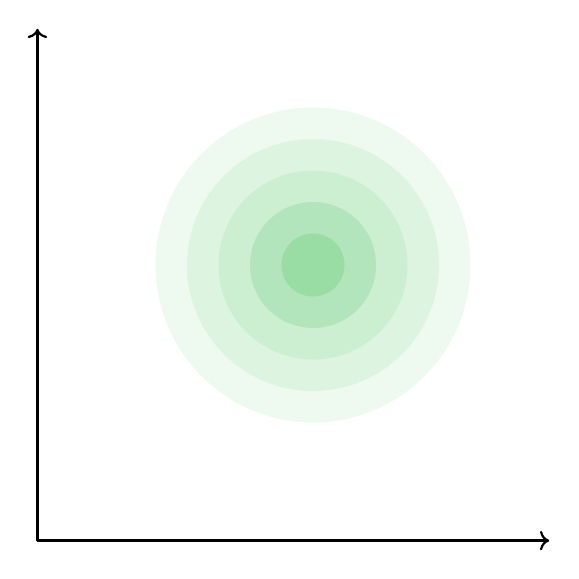
\begin{tikzpicture}
            \draw[thick,->] (-3.5, -3.5) -- (-3.5, 3);
            \draw[thick,->] (-3.5, -3.5) -- (3, -3.5);
            \foreach \x/\alpha in {2/10, 1.6/20, 1.2/30, 0.8/45, 0.4/60}
                \fill[viridisgreen!\alpha] (0, 0) circle (\x);
            %\node[draw, fill=viridisgreen!10] (kde-outer) at (0, 0) {} circle (2) {};
        \end{tikzpicture}
    };
    
    \node[dot, fill=darkgreen!80,
    above right = 0.25cm and 0.3cm of kde,
    label=above:{$h_{\psib}(\x)$}
    ] (s-star) at (kde) {};
    \node[dot, 
    fill=errorcolor!80, 
    below left = -1.5cm and -1.4cm of kde,
    label=below:{$h_{\psib}(\observed{\x})$}
    ] (s-obs) {};
    
    \node[network-box, right = of kde] (inference-network) {$\huge{f_{\phib}}$\\Inference\\Network};
    

    \matrix[right = of inference-network, row sep = 0.2cm] {
    \node[posterior-box, fill=viridisgreen!20]  (correct-posterior) {Correct\\Posterior}; \\ 
    \node[posterior-box, fill=errorcolor!20] (incorrect-posterior) {Incorrect\\Posterior}; \\
    };

    %\node[posterior-box, above right = of inference-network, fill=darkgreen!20] (correct-posterior) {Correct Posterior};
    %\node[posterior-box, below = of correct-posterior, fill=errorcolor!20] (incorrect-posterior) {Incorrect Posterior};
    
    \draw [dashed, thick] (typical-generative-set) -- (x-obs) node [sloped,midway](M){};;
    
    \node[below left = of M] (simulation-gap) {Misspecification};
    \draw [arrow] (simulation-gap)  -- (M);
    
    \node[below left=-2.6cm and -2.6cm of kde] (kde-outer) {};
    \draw [dashed, thick] (s-obs) -- (kde-outer) node [sloped,midway](M2){};;
    
    \node[below right = 2cm and 0.3cm of M2] (simulation-gap-detected) {Misspecification detected};
    \draw [arrow] (simulation-gap-detected)  -- (M2);
    
    
    \draw [arrow, dashed] (x-star) -- (summary-network);
    \draw [arrow, dashed, color=errorcolor] (x-obs) -- (summary-network);
    
    \draw [arrow, dashed] (summary-network) -- (s-star);
    \draw [arrow, color=errorcolor, dashed] (summary-network) -- (s-obs);
    
    %\node[below right = of s-obs] (simulation-gap-detected) {Simulation gap detected};
    %\draw [arrow] (simulation-gap-detected) -- (s-obs);
    
    \draw [arrow, dashed] (s-star) -- (inference-network);
    \draw [arrow, dashed, color=errorcolor] (s-obs) -- (inference-network);
    
    \draw [arrow, dashed] (inference-network) -- (correct-posterior.west);
    \draw [arrow, color=errorcolor, dashed] (inference-network) -- (incorrect-posterior.west);
\end{tikzpicture}

    \end{adjustbox}
    \caption{Conceptual overview of our neural approach.
    The summary network $h_\psi$ maps observations $\x$ to summary statistics $h_\psi(\x)$, and the inference network $f_\phi$ estimates the parameter posterior $p(\thetab\given\x,\mathcal{M})$ from the summary statistics.
    The generative model $\mathcal{M}$ creates training data $\x$ in the green region, and the networks learn to map these data to well-defined summary statistics and posteriors (green regions/dot/box).
    If the generative model $\mathcal{M}$ is misspecificed, real observations $\observed{\x}$ fall outside the training region and are therefore mapped to outlying summary statistics and potentially incorrect posteriors (red dots/box).
    %Conceptual overview of our approach towards trustworthy simulation-based inference with neural density estimators.
    %A summary network $h_{\psib}$ transforms the typical generative set $\mathcal{T}{(\M)}$ of a complex model $\M$ into the typical set of a simple distribution (\eg, Gaussian).
    %Simulation gaps between the model-implied distribution of observables $p(\x \given \mathcal{M})$ and the one implied by reality $p^*(\x)$ manifest themselves as detectable anomalies, causing posterior errors by the inference network $f_{\phib}$.
    Since learning enforces the inlier summary distribution to be known (\eg, a unit Gaussian), misspecification can be detected by a distribution mismatch in summary space, as signaled by a high maximum mean discrepancy \citep[MMD;][]{Gretton2012} score.}
    \label{fig:conceptual}
\end{figure*}

In this paper, we conduct an extensive error analysis of SNPE-C and BayesFlow, two major deep learning algorithms for {\em amortized} approximation of $p(\thetab\given\x,\mathcal{M})$.
We specifically study their accuracy under model misspecification, where the generative model $\mathcal{M}^*$ at test time (the ``true data generating process'') deviates from the one used during training (\ie, $\mathcal{M}^*\ne\mathcal{M}$), a situation commonly known as a {\em simulation gap}. 
Our investigations complement existing work on deep amortized SBI, whose main focus has been on network architectures and training algorithms achieving high accuracy in the well-specified case $\mathcal{M}^*=\mathcal{M}$ \cite{ramesh2022gatsbi, pacchiardi2022likelihood, contrastive, bayesflow, apt, bayes_lstm, papamakarios2016fast}.

\autoref{fig:exp:ddm:stan-bf} illustrates the difference between the two situations:
When the model is well-specified, the posterior estimates of BayesFlow and a classical MCMC sampler \citep[implemented in Stan;][]{Stan2022} are essentially equal, whereas both approaches disagree considerably under model misspecification.
In order to avoid drawing incorrect conclusions from misspecified models and incorrect posteriors, it is of crucial importance to detect whether $\mathcal{M}^*\ne\mathcal{M}$ and to quantify the severity of the mismatch.
However, this is difficult in practice because the true data generating process $\mathcal{M}^*$ is generally unknown (except in controlled validation settings).
\begin{figure}
\centering
    \begin{minipage}{.40\linewidth}
        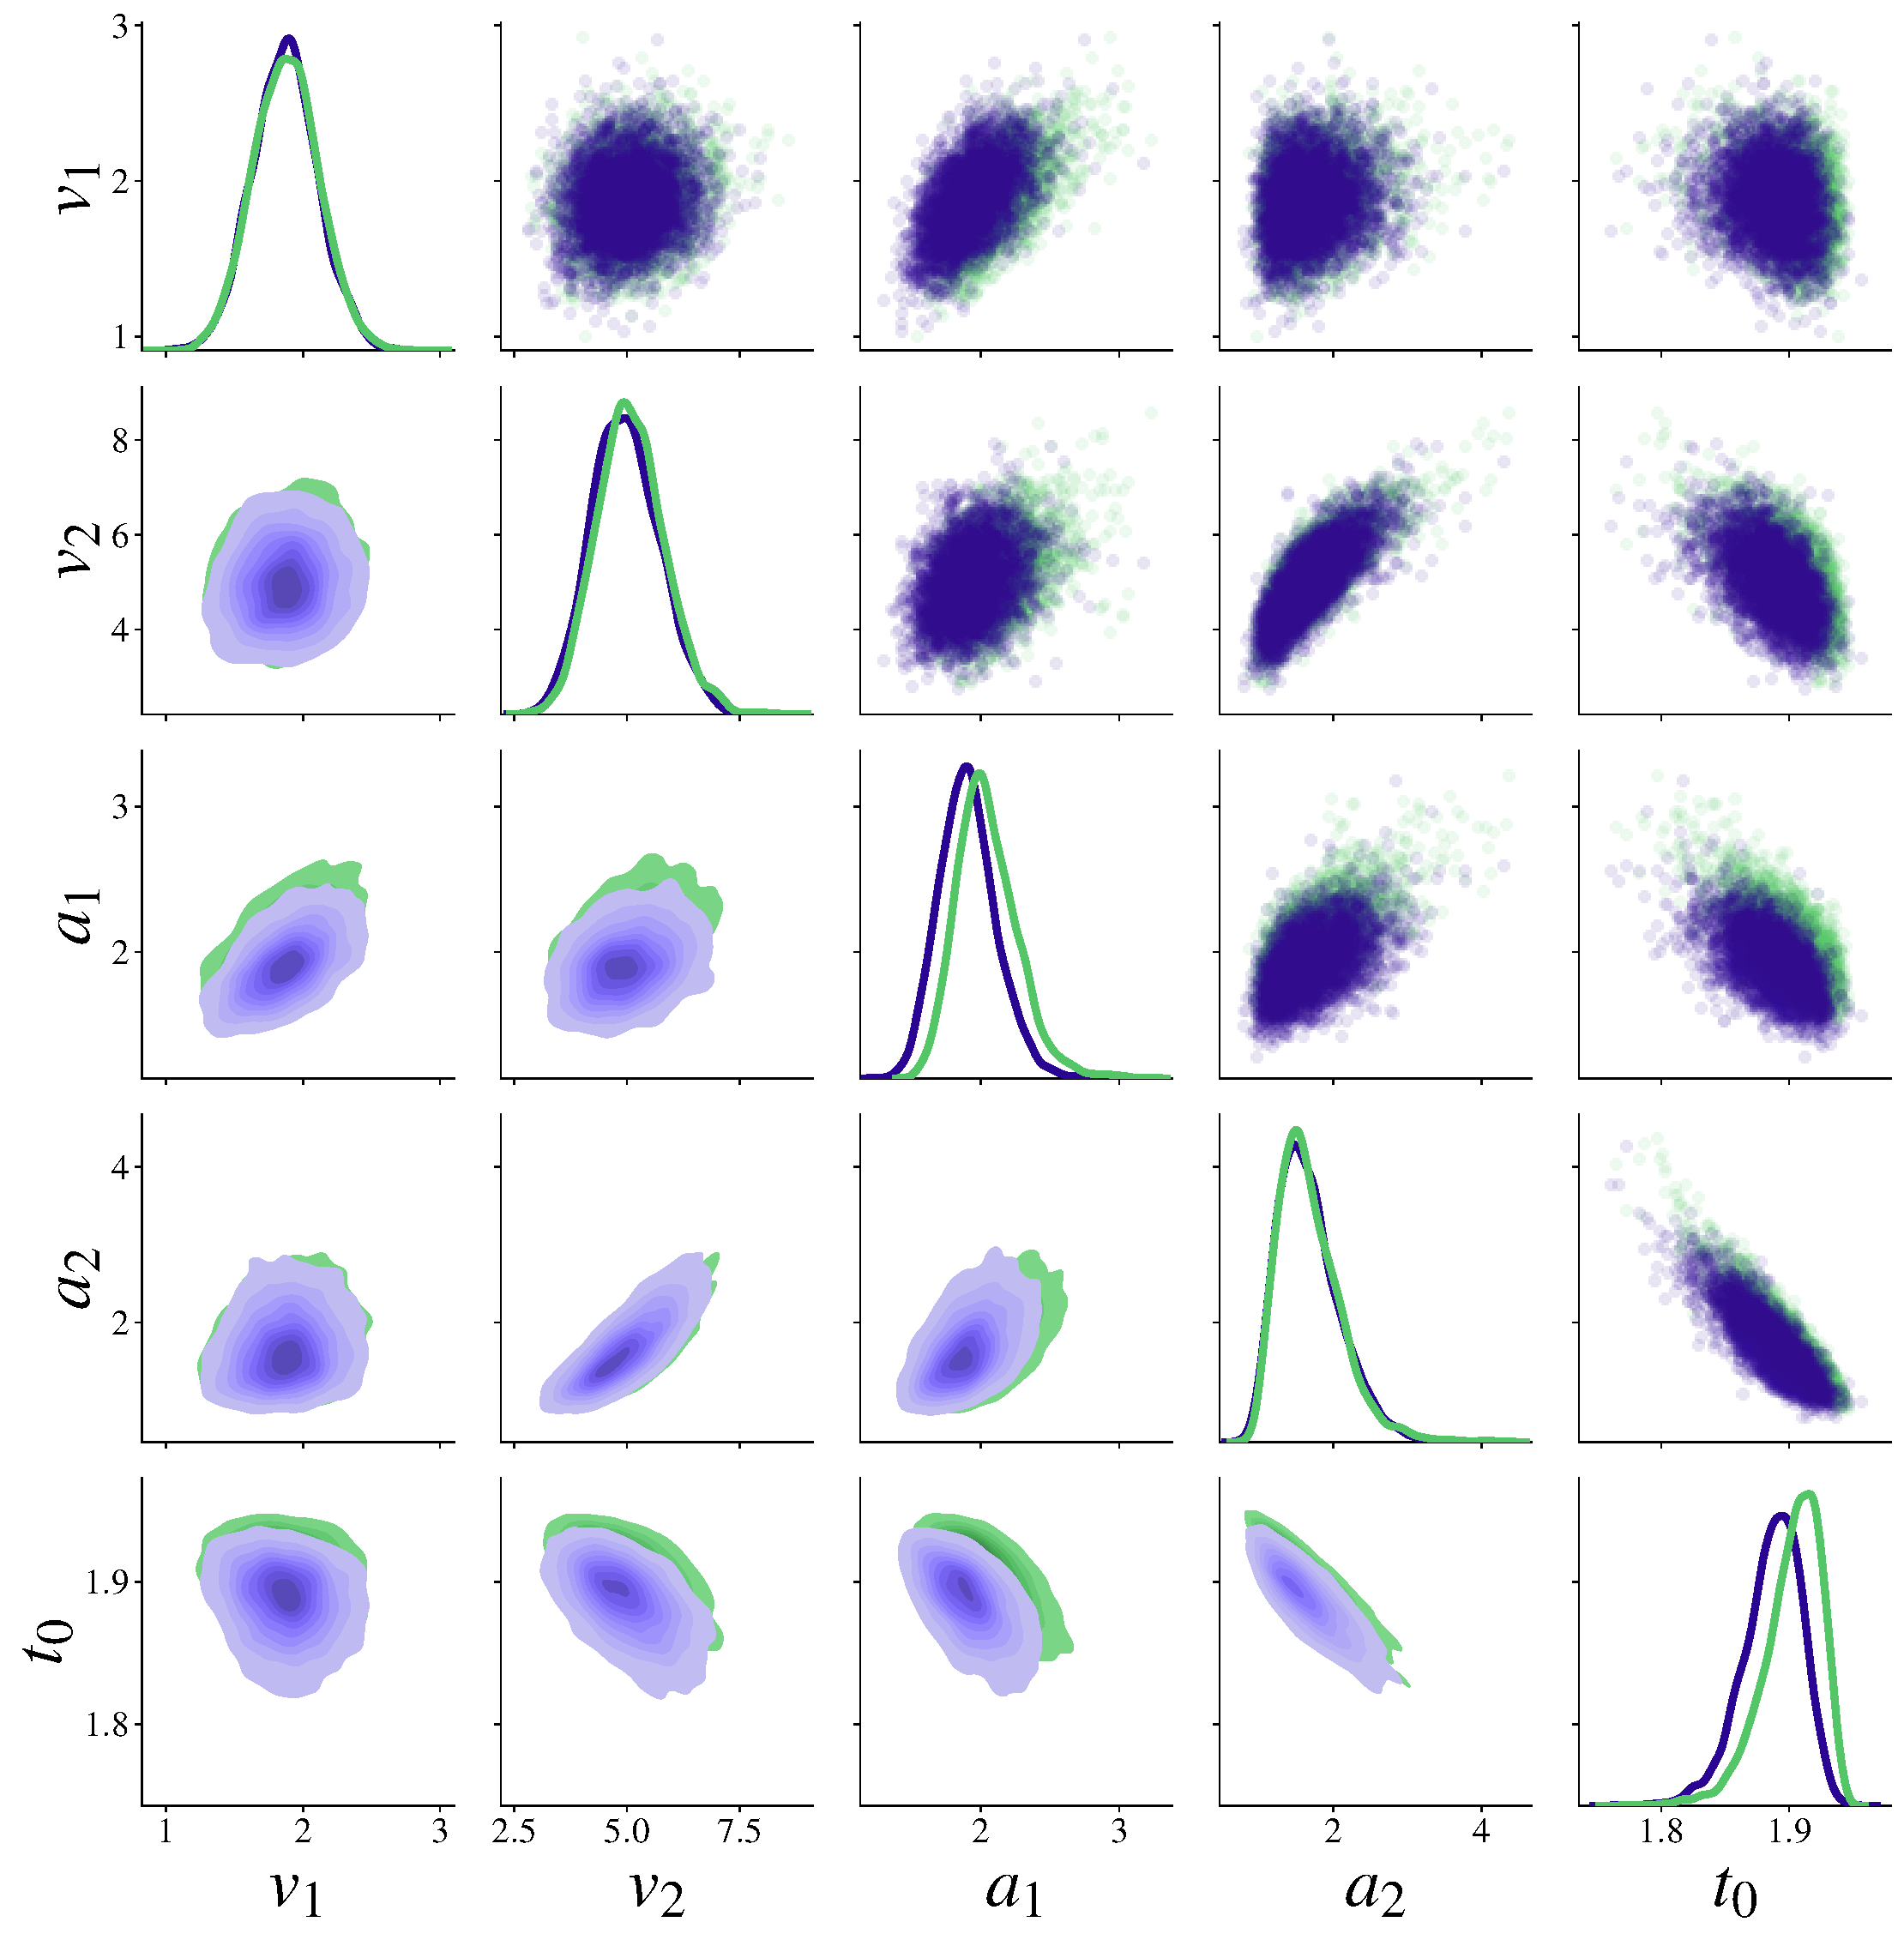
\includegraphics[width=\linewidth]{abf_ddm_unbounded_pairplot_stan_bf_clean.pdf}
    \end{minipage}
    \hspace*{2cm}
    \begin{minipage}{.40\linewidth}
        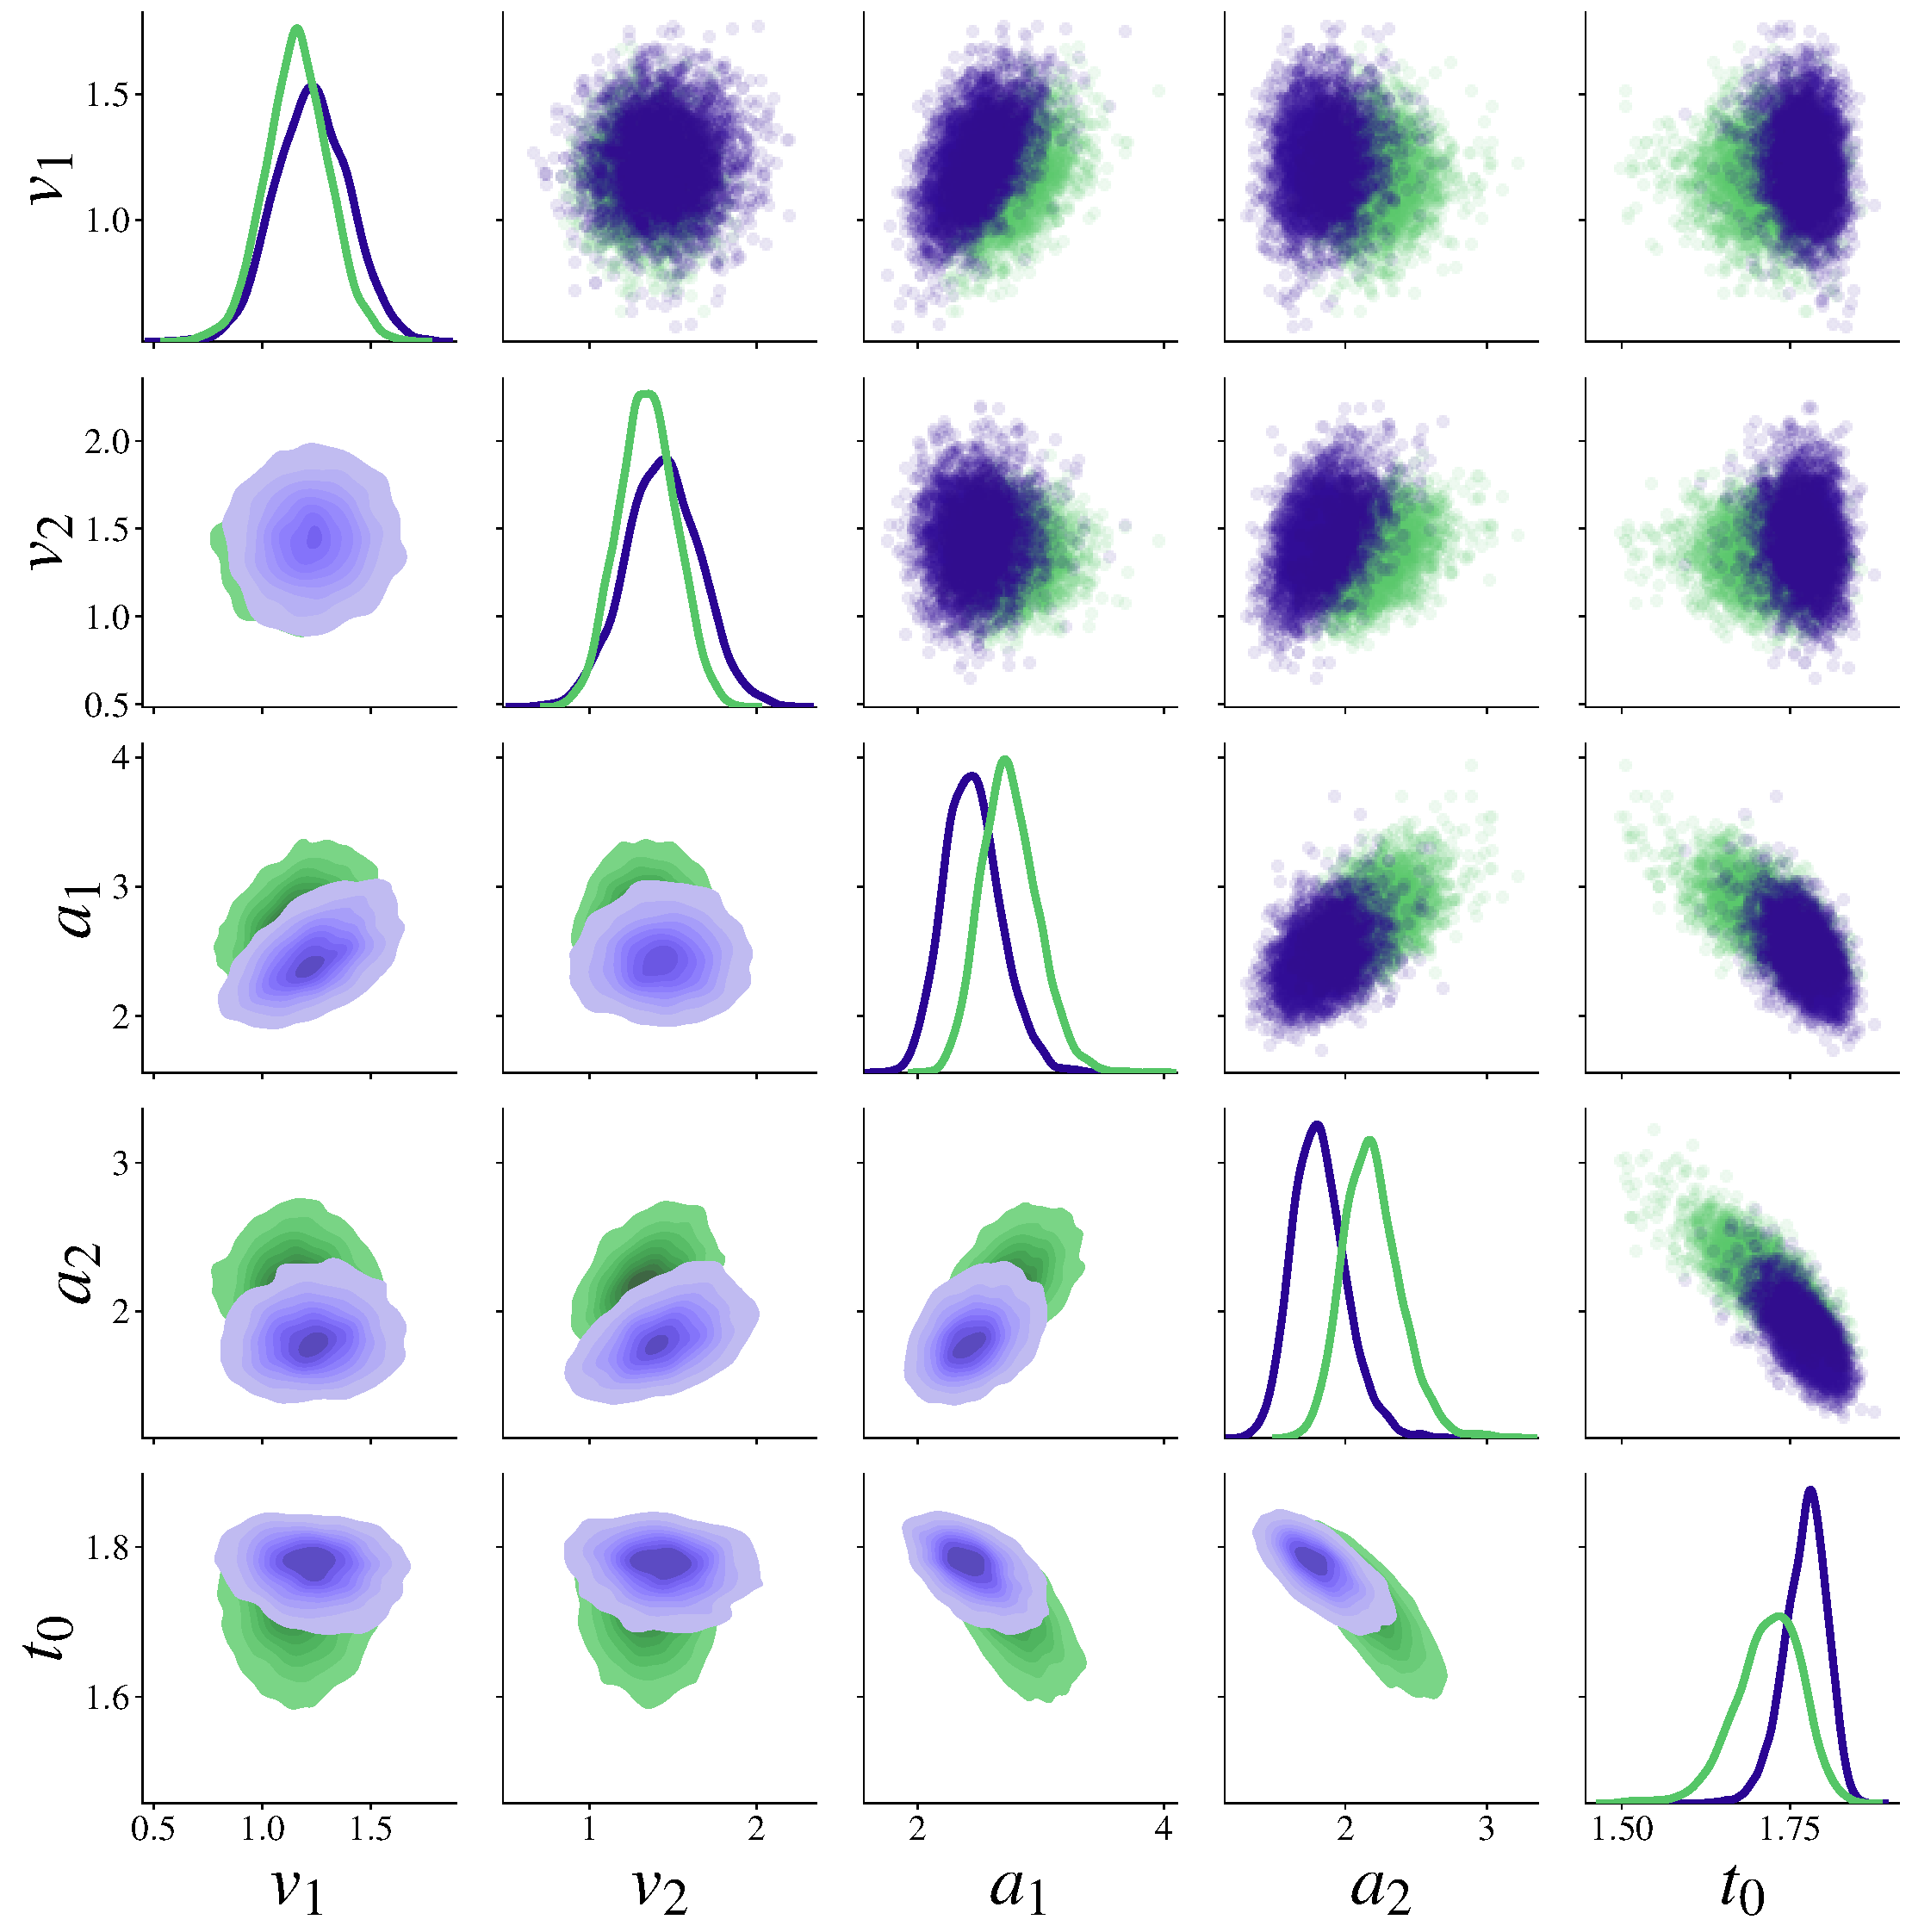
\includegraphics[width=\linewidth]{abf_ddm_unbounded_pairplot_stan_bf_slow.pdf}   
    \end{minipage}\\
    \begin{minipage}{.40\linewidth}
        
\includegraphics[width=\linewidth]{abf_ddm_unbounded_pairplot_stan_bf_legend_clean.pdf}
    \end{minipage}\\
    \begin{minipage}{.45\linewidth}
        \begin{subfigure}[t]{\linewidth}
            \caption{Well-specified: Similar posteriors.}
            \label{fig:exp:ddm:stan-bf:clean}
        \end{subfigure}
    \end{minipage}
    \hfill
    \begin{minipage}{.45\linewidth}
        \begin{subfigure}[t]{\linewidth}
            \caption{Misspecified: Dissimilar posteriors.}
            \label{fig:exp:ddm:stan-bf:slow}
        \end{subfigure}
    \end{minipage}
    \caption{Preview of \textbf{Experiment \numberDDM} on reaction time modeling in psychological experiments (Section~\ref{sec:ddm-experiment}). Posteriors obtained via MCMC (Stan) and simulation-based inference (SBI; BayesFlow) are very similar when the model is well-specified (left).
    However, a simulation gap (here: not accounting for occasional slow responses due to mind wandering) leads to considerable disagreement between these methods (right).
    }
    \label{fig:exp:ddm:stan-bf}
\end{figure}    

In this work, we propose a new misspecification measure that can be trained in an unsupervised fashion (\ie, without knowledge of $\mathcal{M}^*$ or training data from the true data distribution $p^*(\x)$) and reliably quantifies by how much $\mathcal{M}^*$ deviates from $\mathcal{M}$ at test time.
\autoref{fig:conceptual} illustrates how we achieve this by splitting the task between two neural networks, the summary network $h_\psi$ and the inference network $f_\phi$.
This allows us to measure the misspecification in summary space, where it amounts to a distribution mismatch test that can be elegantly implemented by maximum mean discrepancy \citep[MMD;][]{Gretton2012}.

In principle, we could detect misspecification directly in observation space by measuring the discrepancy between the true distribution $p^*(\x)$ and the model marginal $p(\x\given\mathcal{M})$.
However, this is a much harder learning problem, because $p^*(\x)$ and $p(\x\given\mathcal{M})$ are usually complex high-dimensional distributions.
Moreover, $\x$ often has variable dimension in practice (\eg, due to a varying number of observations for different subjects or a varying number of time steps in different time series), which further complicates learning in observation space.
In contrast, the summary space is designed to have fixed and typically low dimension, and end-to-end training of the two networks ensures that the learned summary statistics are maximally informative about $\x$ and follow a simple known distribution (a unit Gaussian) with meaningful MMD scores for misspecification detection.
At the same time, summary-based detectors avoid an important shortcoming of traditional Bayesian model checking methods \citep[e.g.,][]{bayes_ppc}, which base their diagnostics on the posterior distributions $p(\thetab\given\x,\mathcal{M})$ and therefore become unreliable if these posteriors get distorted in unpredictable ways under model misspecification (cf.\ \autoref{fig:exp:ddm:stan-bf:slow}).

Our experiments clearly demonstrate the power of our new measure both on toy examples with an analytical ground-truth, and on representative scientific tasks in cell biology, cognitive decision making, and disease outbreak dynamics.
We show how amortized posterior inference gradually deteriorates as the simulation gap widens and how the proposed misspecification test warns users about suspicious outputs, raises an alarm when predictions are not trustworthy, and guides model designers in their search for better simulators.

In particular, our paper makes the following key contributions:
\begin{enumerate}[label=(\roman*)]
    \item We systematically conceptualize different sources of model misspecification in amortized Bayesian inference with neural networks and propose a new detection criterion that is widely applicable to different model structures, inputs, and outputs.
    \item We incorporate this criterion into existing amortized neural posterior estimation methods, both with hand-crafted and learned summary statistics, and extend the associated learning algorithms in a largely non-intrusive manner.
    \item We conduct a systematic empirical evaluation of our detection criterion, the influence of the summary space dimension, and the relationship between summary outliers and posterior distortion under various types and strengths of model misspecification.
\end{enumerate}

%Detecting such deviations is of crucial importance because mild or sometimes severe mismatch between simulated and actual behavior occurs almost inevitably in practice.
%To formalize and demonstrate our approach, we develop a theoretical basis for misspecification detection, incorporate it into SBI frameworks with both learned and hand-crafted summary statistics, and investigate its performance on toy examples with analytical ground-truth, as well as representative scientific tasks in cell biology, cognitive decision making, and disease outbreak dynamics.
% (i) Diffusion models are popular in psychology to decompose human decision processes into cognitive parameters, such as speed of information processing, cautiousness, and non-decisional factors \cite{diffusion}.
% These parameters must be estimated from response-time experiments, but diffusion models may not always fit human decision processes accurately. 
% (ii) Compartmental models such as SIR are a mainstay of epidemiology \cite{compartment}. 
% They represent hidden disease dynamics by transitions between groups of people with different properties.
% The transition parameters of real diseases like Covid-19 are estimated from reported incidence data, but the details of the simulation design (\eg, the number and type of compartments or the handling of reporting errors and counter-measure effects) leave plenty of room for mo del mismatch. 
\begin{comment}
Recently, deep generative neural networks (DGNNs) were introduced as promising SBI tools in various scientific domains (see \cite{frontier} for a review).
During training, DGNNs are presented with a large number of simulations to learn the relationship between simulation outcomes and the underlying parameters or parameter posteriors.
When properly converged, DGNNs can generalize this knowledge to unseen simulated or real observations and infer the corresponding unknown parameters.
The training effort thus \emph{amortizes} quickly over multiple inference queries, in contrast to traditional sampling methods (\eg, MCMC), which cannot leverage experience and must re-run their expensive computations from scratch for each observed data set.
Importantly, DGNNs are capable of fully Bayesian inference, that is, they can perform uncertainty quantification within a self-consistent probabilistic framework \cite{gelman1995bayesian}.
This complements existing work on deep amortized SBI, which has mainly focused on finding network architectures and training algorithms maximizing accuracy in the well-specified case \cite{ramesh2022gatsbi, pacchiardi2022likelihood, contrastive, bayesflow, apt, bayes_lstm, papamakarios2016fast}.

In contrast, the consequences of \emph{model misspecification} remain largely unsolved in the context of \emph{amortized} SBI.
Model misspecification occurs when a model does not fully represent the actual behavior of the modeled system or when it does not completely account for measurement errors and contamination in the observations serving as inference inputs.
In the context of SBI, this predicament is also referred to as a \emph{simulation gap}, and we use the terms interchangeably.
%Simulation gaps are especially critical for neural networks, since training data from misspecified models may translate into incorrect generalizations at test time.

%The above limitation does not exist for classical Bayesian inference methods, such as MCMC \cite{nuts}.
%Under certain regularity conditions, they enjoy the guarantee that the obtained samples represent the \emph{true parameter posterior} even when the model is misspecified \cite{nuts}.
Amortized Bayesian methods require simulations to be faithful proxies of reality and might yield \emph{wrong posteriors} when presented with observables which are atypical under the assumed model (cf.\ \autoref{fig:conceptual}).
Our experiments clearly demonstrate this effect and show how amortized posterior inference gradually deteriorates as the simulation gap widens.
Consequently, amortized SBI methods must be able to detect simulation gaps and subsequent posterior errors, so that they can warn users about suspicious outputs (or even decline to make predictions under such circumstances) and guide model designers in their search for better simulators.

Traditional Bayesian model checking methods \cite[e.g.,][]{bayes_ppc} are not applicable here, because they may obscure deficiencies in the parameter posteriors (\eg, over- or underconfidence) and, more importantly, require correct posteriors to begin with.
Reliable model misspecification detection is therefore a crucial prerequisite for trustworthy simulation-based inference with amortized deep learning methods.

The main purpose of this paper is twofold. 
First, we conceptualize model misspecification in applications of simulation-based Bayesian inference with neural networks (Section \ref{sec:defining-model-misspecification}). 
We then propose a simple and intuitive way to detect model misspecification and posterior inference errors (posterior errors, for short) arising due to finite training (Section \ref{sec:posterior-inference-errors}). A conceptual illustration is provided in \autoref{fig:conceptual}.
Our approach does not modify existing neural architectures and greatly benefits from the properties of amortized inference. 
Instead, it acts as a modular and intuitive extension of previous work on amortized neural approximators towards a principled simulation-based Bayesian workflow \cite{ramesh2022gatsbi, pacchiardi2022likelihood, bayesflow, apt, bayes_lstm, papamakarios2016fast}.
Indeed, the demand for a trustworthy workflow in amortized Bayesian inference increases heavily due to the growing number of applications relying on amortized simulation-based inference \citep[e.g., ][]{butter2022machine, covid_germany, gonccalves2020training, bayesflow_agent, bayesflow_qcd, von_krause_mental_2022, ghaderi-kangavari_general_2022}. 
In particular, the key contributions of our paper are thus:
\begin{enumerate}[label=(\roman*)]
    \item A way to conceptualize different sources of model misspecification in amortized Bayesian inference with neural networks;
    \item An augmented optimization objective and an easy-to-use criterion to detect model misspecification and posterior errors during inference, regardless of a model's structure, input, or output;
    \item A systematic investigation of our detection criterion and its relationship with posterior errors and the number of summary statistics in a variety of models and misspecifications.
\end{enumerate}
\end{comment}

\section{Related Work}\label{sec:related-work}
Model misspecification has been studied both in the context of standard Bayesian inference and generalizations thereof \citep[i.e., generalized Bayesian inference, see][]{knoblauch2019generalized, schmon_generalized_2021}.
To alleviate model misspecification in generalized Bayesian inference, researchers have investigated probabilistic classifiers \citep{mms_genbayes}, second-order PAC-Bayes bounds \citep{masegosa2020learning}, scoring rules \citep{giummole2019objective}, priors over a class of predictive models \citep{loaiza2021focused}, or Stein discrepancy as a loss function \citep{matsubara_robust_2022}.
Notably, most of these approaches deviate from the standard Bayesian formulation and investigate alternative schemes for belief updating and learning (e.g., replacing the likelihood function with a generic loss function).
In contrast, our method remains grounded in the standard Bayesian framework embodying an implicit likelihood principle \cite{berger_likelihood_1988}.
Differently, power scaling methods incorporate a modified likelihood (raised to a power $0 < \alpha < 1)$ in order to prevent potentially overconfident Bayesian updating \cite{bayesian_miss, holmes2017assigning}.
However, the SBI setting assumes that the likelihood function is not available in closed-form, which makes an explicit modification of the implicitly defined likelihood less obvious.

Neural approaches to amortized SBI can be categorized as either targeting the posterior \cite{bayesflow, apt}, the likelihood \cite{snle, ratios}, or both \cite{snpla}.
These methods employ simulations for training amortized neural approximators which can either generate samples from the posterior directly \cite{bayesflow, apt, snpla} or in tandem with Markov chain Monte Carlo (MCMC) sampling algorithms \cite{snle, ratios}.
Since the behavior of these methods depends on the fidelity of the simulations used as training data, we hypothesize that their estimation quality will be, in general, unpredictable, when faced with atypical real-world data.
Indeed, the critical impact of model misspecification in neural SBI has been commonly acknowledged in the scientific research community \cite{cannon_investigating_2022, alquier_concentration_2019, zhang_convergence_2020, frazier_model_2020, frazier_robust_2021, pacchiardi_score_2022}.

Recent approaches to detect model misspecification in simulation-based inference are usually based on the obtained approximate posterior distribution \citep[e.g.,][]{hermans2021averting, dellaporta_robust_2022, leclercq_simulation-based_2022}.
However, we show in \textbf{Experiment \numberGaussianMeans} and \textbf{Experiment \numberDDM} that the approximate posteriors in simulation-based inference tend to show pathological behavior under misspecified models. 
Posteriors from misspecified models may erroneously look legitimate, rendering diagnostic methods on their basis unreliable.
Moreover, the same applies for approaches based on the \textit{posterior predictive distribution} \citep{burkner_approximate_2020, gabry_visualization_2019, vehtari_survey_2012} since these also rely on the fidelity of the posterior distribution and can therefore only serve as an indirect measure of misspecification.

A few novel techniques aim to \emph{mitigate} model misspecification in simulation-based inference to achieve robust inference.
\citet{delaunoy_towards_2022} equip neural ratio estimation \cite{ratios} with a balancing condition which tends to produce more conservative posterior approximations.
\citet{ward_robust_2022} explore a way to alleviate model misspecification with two neural approximators and subsequent MCMC.
While both approaches are appealing in theory, the computational burden of MCMC sampling contradicts the idea of amortized inference and prohibits their use in complex applications with learned summary statistics and large amounts of data.
In fact, \citet{von_krause_mental_2022} recently used amortized neural SBI on more than a million data sets and demonstrated that an alternative inference method involving non-amortized MCMC would have taken years of sampling per model.
% When operating in a non-amortized manner, sequential neural posterior estimation \citep[SNPE; \eg,][]{apt} methods might be less exposed to the effects of simulation gaps. 
% SNPE methods iteratively transform a proposal distribution into an approximate posterior and thus progressively narrow down the scope of plausible simulations informed by actual observations.
% However, the behavior and correctness of SNPE methods under simulation gaps has not yet been analyzed.

For robust non-amortized ABC samplers, the possibility of utilizing hand-crafted summary statistics as an important element of misspecification analysis has already been explored \cite{frazier_model_2020, frazier_robust_2021}.
Our work parallels these ideas and extends them to the case of \textit{learnable summary statistics} in amortized SBI on potentially massive data sets, where ABC becomes infeasible.
However, we show in \textbf{Experiment \numberCS} that our method also works with hand-crafted summary statistics.
Furthermore, we offer a conceptual discussion on the sources of misspecifications (and their consequences) arising in amortized SBI and explore the connection between posterior errors and model misspecification as a function of the number of summary statistics.

In the field of variational Bayes, recent work has studied the convergence and concentration rates with and without misspecification \cite{alquier_concentration_2019, zhang_convergence_2020}.
These approaches are not directly transferable to amortized models because the methods used in variational Bayes do not naturally provide a practical ``misspecification alarm'', which is needed because neural approximators remain unchanged after the training phase in SBI.

Framing Bayesian model selection as classification \cite{ruff_deep_2018, pudlo2016reliable}, diverse outlier detection techniques seem viable for uncovering simulation gaps in model comparison settings.
\citet{amortized_bmc} propose to train regularized evidential networks which learn a higher-order distribution over posterior model probabilities. 
This way, conclusions about the ``absolute misfit'' of all models in a set of candidate models can be drawn.
However, this approach is not suitable for parameter estimation and currently requires a loss function which does not guarantee a correct approximation of posterior model probabilities. 

Finally, from the perspective of deep anomaly detection, our approach for learning informative summary statistics can be viewed as a special case of \emph{generic normality feature learning} \cite{pang_deep_2022}. 
Standard learned summary statistics are optimized with a generic feature learning objective which is not primarily designed for anomaly detection \citep{bayesflow}.
However, since learned summary statistics are also optimized to be maximally informative for posterior inference, they are forced to capture underlying data regularities \cite{pang_deep_2022}.
This makes the summary statistics equipped with a tractable \textit{latent summary space} appropriate targets for misspecification detection.
% once our extended optimization objective from \autoref{eq:bf_kl_mmd} is employed.

\section{Method}\label{sec:methods}
This section defines model misspecification as a mismatch between marginal distributions and explains the building blocks and theoretical implications of our proposed detection method in the context of amortized SBI.
To shorten notation throughout the manuscript, we use an abbreviated set notation $\smash{\{\boldsymbol{a}^{(n)}\}\equiv\{\boldsymbol{a}^{(n)}\}_{n=1}^N}$, since we use the same lowercase and uppercase letter for referencing a set member and denoting set size respectively (e.g., $n \in \{1,\dots,N\})$.
% xi vs theta
% how to change xi and not g -> 
% Joint distribution -> highlight 
% Move up -> then discuss parameter vs data, and why inspection of parameter space senseless is -> motivate, deviations in theta are deviations in data, posterior not useful -> wrong in the decisive moment, train together
\subsection{Defining Model Misspecification}\label{sec:defining-model-misspecification}
For the purpose of simulation-based inference, we define a generative model as a triple $\mathcal{M} = \big( \model, \noised, \prior \big)$.
Such a model generates data $\x \in \mathcal{X}$ according to the system
\begin{equation}
    \x = \model \quad\textrm{with}\quad \xib \sim \noised,\; \thetab \sim \prior,
\end{equation}
where $g$ denotes a (randomized) simulator, $\xib \in \Xi$ is a source of randomness (\ie, noise) with density function $\noised$, and $\prior$ encodes prior knowledge about plausible simulation parameters $\thetab \in \Theta$.
Intuitively, $\x$ represents quantities that we can observe and measure.
We use the decorated symbol $\observed{\x}$ to mark data that was in fact \emph{observed} in the real world and not merely simulated by the assumed model $\M$.
The parameters $\thetab$ consist of hidden properties whose role in $g$ we explicitly understand and model, and $\xib$ takes care of nuisance effects that we only treat statistically.
The abstract spaces $\mathcal{X}, \Xi$, and $\Theta$ denote the domain of possible output data (possible worlds), the scope of noise, and the set of admissible model parameters, respectively.
The distinction between hidden properties $\thetab$ and noise $\xib$ is not entirely clear-cut, but depends on our modeling goals and may vary across applications.
Moreover, our understanding of the world is constantly evolving, and yesterday's noise might become tomorrow's signal.

Whenever we employ simulations to investigate some real world phenomenon, a close correspondence between model and reality is necessary. 
Unacceptably large discrepancies between the two realms are known as a \emph{simulation gap}, and the corresponding model is said to be \emph{misspecified}.
Model misspecification can arise from any of the three model components in isolation or simultaneously.
A few illustrative examples show what can go wrong in practice:

\begin{enumerate}[label=(\roman*)]
    \item \textbf{Misspecified Simulator.} In a model for the hydraulic conductivity of a medium, the spatial composition of the material is essential: A simulator relying on the assumption of homogeneity will wrongly predict the behavior of heterogeneous materials, biasing inference results in complex and arbitrary ways \citep{Schoniger2015, Nowak2016}.
    \item \textbf{Unexpected Contamination.} During an ongoing pandemic, data collection may be severely distorted, for example by noisy measurements, systematic underreporting, and delayed data transfer \cite{covid_germany}, to name just a few.
    An epidemiological model disregarding these factors in $\noised$ will produce erroneous inferences about key disease parameters, even if the underlying theory was otherwise a good approximation of the disease dynamics.
    \item \textbf{Misspecified Prior.} When the admissible region of the prior $\prior$ is specified too large---for example, allows negative mass---physically impossible simulations may arise.
    On the other hand, when the prior is too narrow, the typical generative set of a model may leave out an important subset of observables or lead to unreasonable uncertainty estimates \citep[e.g., in satellite retrievals;][]{nguyen2019sensitivity}.
\end{enumerate}

Our generative model formulation is equivalent to the standard factorization of the Bayesian joint distribution into likelihood and prior, $\jointm = \likm\,\priorm$, where $\mathcal{M}$ expresses the prior knowledge and assumptions embodied in the model.
The likelihood is obtained by marginalizing the joint distribution $p(\xib, \x \given \thetab, \mathcal{M})$ over all possible values of the nuisance parameters $\xib$, that is, over all possible execution paths of the simulation program, for fixed $\thetab$:
\begin{equation}
    \likm = \int_{\Xi} p(\xib, \x \given \thetab, \mathcal{M})\,\diff \xib.
\end{equation}
This integral is typically intractable \cite{frontier}, but we assume that it exists and is non-degenerate, that is, it defines a proper density over the constrained manifold $\left(g(\thetab, \xib), \xib\right)$.%, and this density can be learned.
Whenever we model a real-world complex system, we assume an unknown (true) generator $\M^*$, which yields an unknown (true) distribution $\observed{\x} \sim p^*(\x)$ and is available to the data analyst only via a finite realization (\ie, actually observed data $\observed{\x}$).
Then, using the Bayesian formulation, we say that a generative model $\mathcal{M}$ is \emph{strictly} well-specified if
\begin{equation}\label{eq:spec}
    p^*(\x) = p(\x \given \mathcal{M}) \equiv \int_{\Theta} \likm\,\priorm\,\diff\thetab 
\end{equation}
for every $\x \in \mathcal{X}$.
Conversely, a generative model is misspecified if an observable $\x \in \mathcal{X}$ exists for which the above equality is violated. 

Note that our definition of model misspecification does not assume the existence of a \textit{true} parameter vector $\thetab^*$, as required by some definitions relying on asymptotic guarantees \cite{vandervaart2000asymptotic}. 
That is, we do not require that the (conditional) likelihood itself matches the assumed data-generating distribution, which would mean $p^*(\x) = p(\x \given \thetab^*, \mathcal{M})$ for some ground-truth $\thetab^*\in\Theta$.
Instead, we focus on the \textit{marginal likelihood} $p(\x \given \mathcal{M})$ which represents the entire prior predictive distribution of a model and does not commit to a single most representative parameter vector \cite{lotfi2022bayesian, masegosa2020learning}.
In this way, multiple models whose marginal distributions are representative of $p^*(\x)$ can be considered well-specified without any reference to some hypothetical ground-truth $\thetab^*$, which may not even exist for opaque systems with unknown parameters.

Since models necessarily simplify reality, the above strict criterion for well-specified models in Eq.~\ref{eq:spec} is often unattainable in practice.
We therefore relax the requirement by quantifying a model's degree of misspecification in terms of the information loss incurred by the following simplification:
For an acceptable upper bound $\vartheta$ on the information loss, a model is well-specified if $\mathbb{D}\big[p^*(\x)\,||\,p(\x \given \mathcal{M})\big] < \vartheta$
%\begin{equation}
%    \mathbb{D}\big[p^*(\x)\,||\,p(\x \given \mathcal{M})\big] < \vartheta \label{eq:mms}
%\end{equation}
and misspecified otherwise. 
The symbol $\mathbb{D}$ denotes a divergence metric quantifying the ``distance'' between the data distributions implied by reality and by the model (the marginal likelihood). 
Notably, equality in Eq.~\ref{eq:spec} implies no information loss by modeling $p^*(\x)$ with $p(\x \given \mathcal{M})$ and thus leads to a divergence of zero.
A natural choice for $\mathbb{D}$ would be a metric from the family of $\mathcal{F}$-divergences, such as the Kullback-Leibler (KL) divergence. 
However, since the practical computation of $\mathcal{F}$-divergences requires closed-form densities, and thus $p^*(\x)$ to be analytically tractable, we prefer a probability integral metric, such as the Maximum Mean Discrepancy \citep[MMD;][]{Gretton2012}. Using the kernel trick, the MMD can be expressed as
\begin{equation}\label{eq:MMD:MMD-kernel-trick}
    \mathbb{MMD}^2\big[p^*(\x)\,||\,p(\x \given \mathcal{M})\big] =
    \mathbb{E}_{
    %x, \x'\sim 
    p^*(\x)}\big[\kappa(\x, \x')\big]
    + \mathbb{E}_{
    %\x, \x'\sim 
    p(\x \given \mathcal{M})}\big[\kappa(\x, \x')\big]
    - 2 \mathbb{E}_{
    \begin{mysubarray}
      \x{\ }&\sim&p^*(\x) 
      \\ 
      \x'&\sim&p(\x \given \mathcal{M})
    \end{mysubarray}
    }\big[\kappa(\x, \x')\big].
\end{equation}
with any positive definite kernel $\kappa(\cdot,\cdot)$.
Crucially, this metric is practically tractable because it can be efficiently estimated via finite samples from $p^*(\x)$ and $p(\x \given \mathcal{M})$, and it equals zero if and only if the two densities are equal \cite{Gretton2012}.

We use sums of Gaussian kernels with different widths $\sigma_i$ as an established and flexible universal kernel \cite{Muandet2017}.
However, \citet{Ardizzone2018} argue that kernels with heavier tails may improve performance by yielding superior gradients for outliers.
Thus, we repeated all experiments with a sum of inverse multiquadratic kernels \citep[as proposed by][]{Tolstikhin2017}, and find that the results are essentially equal.

\subsection{Neural Architectures for Amortized Inference}

Our proposed method can be applied to any framework that uses summary statistics as an input to an amortized posterior approximator \cite{burkner2022some}.
We will exemplarily outline the seamless integration of our method into the BayesFlow \cite{bayesflow} and the SNPE-C \citep[aka APT;][]{apt} frameworks, but our method should also apply to the broader class of scoring-based minimization \cite{pacchiardi2022likelihood} or adversarial \cite{ramesh2022gatsbi} approaches.
BayesFlow and SNPE-C, as implemented in the respective software toolkits \cite{tejero2020sbi}, use different neural architectures and training regimes to minimize the expected KL divergence between approximate and correct simulation posterior
\begin{equation}
    \psib^*,\phib^* = \argmin_{\psib, \phib}\mathbb{E}_{p(\x \given \mathcal{M})}\left[\int_{\Theta} p(\thetab \given \x, \mathcal{M}) \log \frac{p(\thetab \given \x, \mathcal{M})}{q_{\phib}\big(\thetab \given h_{\psib}(\x), \mathcal{M}\big)}\, \diff\thetab\right], \label{eq:kl_bf_m}
\end{equation}
where the expectation is taken with respect to the prior predictive distribution $p(\x \given \mathcal{M})$. 
This criterion reduces to
\begin{equation}
  \psib^*, \phib^* =
  \argmin_{\psib, \phib}  
    \mathbb{E}_{\jointm}\Big[-\log q_{\phib}\big(\thetab\given h_{\psib}(\x), \mathcal{M}\big)\Big], \label{eq:kl_bf}
\end{equation}
since the correct posterior $\postm$ does not depend on the trainable neural network parameters ($\psib$, $\phib$).
The above criterion optimizes a summary (aka embedding or conditioning) network with parameters $\psib$ and an inference network with parameters $\phib$ which jointly amortize a generative model $\M$.
The summary network transforms input data $\x$ of variable size and structure to a fixed-length representation $\z = h_{\psib}(\x)$.
The inference network $f_{\phib}$ generates random draws from an approximate posterior $q_{\phib}$ via a normalizing flow, for instance, realized by a conditional invertible neural network \citep[cINN,][]{Ardizzone2019} or a conditional masked autoregressive flow \citep[cMAF,][]{papamakarios2017masked}.
Accordingly, we can compute the exact posterior density via the change of variable formula:
\begin{equation}
    q_{\phib}(\thetab \given h_{\psib}(\x), \mathcal{M}) = p\Big(f_{\phib}\big(\thetab; h_{\psib}(\x)\big)\Big)\left|\det \left(\frac{\partial f_{\phib}(\thetab;h_{\psib}(\x))}{\partial \thetab}\right)\right| \label{eq:cinn}
\end{equation}
We approximate the expectation in Eq.~\ref{eq:kl_bf} via simulations from the generative model $\M$ and repeat the process until convergence, which enables us to perform fully amortized inference (i.e., the posterior functional can be evaluated for any number of observed data sets $\x$).
Moreover, this objective is self-consistent and results in correct amortized inference under optimal convergence \cite{apt, bayesflow}.
However, simulation-based training (cf.\ Eq.~\ref{eq:kl_bf_m}) takes the expectation with respect to the model-implied prior predictive distribution~$p(\x\given\M)$, not necessarily the ''true`` real-world distribution $p^*(\x)$.
Thus, optimal convergence does not imply correct amortized inference or faithful prediction in the real world when there is a simulation gap, that is, when the assumed training model $\M$ deviates critically from the unknown true generative model $\M^*$.

At this point, we may ask whether the same problem also exists for sequential inference, as realized by multi-round SNPE methods \cite{contrastive, apt}. 
Whenever we require inference for a single observation $\observed{\x}$, we can sequentially transform the prior distribution $\prior$ into the posterior $p(\thetab \given \observed{\x}, \mathcal{M})$ through a series of simulation-based training rounds \citep{contrastive, apt}.
Typically, we will use the approximate posterior after a given round as the proposal prior for the next round, resulting in a \textit{semi-amortized} optimization criterion
\begin{equation}
  \psib^*, \phib^* =
  \argmin_{\psib, \phib}  
    \mathbb{E}_{p(\x \given \thetab, \mathcal{M}) \widehat{p}(\thetab \given \mathcal{M})}\Big[-\log \widehat{q}_{\phib}\big(\thetab \given h_{\psib}(\x), \mathcal{M}\big)\Big], \label{eq:kl_apt}
\end{equation}
where $\widehat{p}(\thetab \given \mathcal{M})$ is the current proposal distribution and the approximate posterior $\widehat{q}_{\phib}$ is represented as a categorical distribution over a discrete set of \textit{atomic proposals} in order to be tractable \cite{apt}.
In this way, the neural approximator specializes for estimating solely the parameters of $\observed{\x}$, since information from the observed data is used to narrow down the prior $\prior$ to the typical set of $\postm$.
Still, the first round in sequential inference depends only on the simulator outputs, so simulation gaps are likely to remain problematic, potentially propagating posterior inference errors through further training rounds. 
Indeed, we demonstrate this behavior in \textbf{Experiment \numberGaussianMeans}.

\subsection{Structured Summary Statistics}\label{sec:structured-summary-statistics}
In simulation-based inference, summary statistics have a dual purpose, because (i) they are fixed-length vectors, even if the input data $\x$ have variable length; and (ii) they usually contain crucial features of the data, which drastically simplifies neural posterior inference.
However, in complex real-world scenarios (such as decision making or COVID-19 modeling, cf.\ \textbf{Experiments \numberDDM} and \textbf{\numberCovid}), it is not feasible to rely on hand-crafted summary statistics.
Thus, combining neural posterior inference with \emph{learned summary statistics} leverages the benefits of summary statistics (i.e., compression to fixed-length vectors) while avoiding the virtually impossible task of designing hand-crafted summary statistics for complex models.

\begin{algorithm}[t]
\caption{Misspecification-aware amortized Bayesian inference. The algorithm illustrates online learning for simplicity. The training phase can utilize any other learning paradigm as well (e.g., round-based). Thus, details like batch size or round indices are omitted in the training phase of the algorithm.}
\label{alg:mms}
\begin{algorithmic}[1]
\State \textbf{Training phase}:
\Repeat
\State Sample parameters and data $(\thetab, \x)$ from the specified generative model $\M$.
\State Pass the data $\x$ through the summary network: $\z = h_{\psib}(\x)$.
% \State Draw samples from unit Gaussian (desired summary space): $\tilde{\z} \sim \mathcal{N}(\0, \mathbb{I})$
% \State Estimate MMD distance of summary statistics to unit Gaussian: $\widehat{\mathrm{MMD}}^2(\z \,||\,\tilde{\z})$.
\State Compute $-\log q_{\phib}\big(\thetab\given \z, \mathcal{M}\big)$ using Eq.~\ref{eq:cinn}.
\State Compute Monte Carlo estimate of Eq.~\ref{eq:bf_kl_mmd} as a loss function.
\State Update neural network parameters $\psib, \phib$  via backpropagation.
\Until{convergence to $\widehat{\psib}, \widehat{\phib}$}
\\
\State \textbf{Inference phase} \textit{(given $N$ observed or test data sets $\{\observed{\x}^{(n)}\}$, query $L$ draws from the amortized posterior, use $M$ draws from the validation summary distribution)}:
\For{$m=1,\ldots, M$}
\State Re-use data set $\x^{(m)}$ from the training phase or simulate a new one from $\mathcal{M}$.
\State Pass the data set $\x^{(m)}$ through the converged summary network: $\z^{(m)} = h_{\widehat{\psib}}(\x^{(m)})$.
\EndFor
\For{$n=1,\ldots, N$}
\State Pass the observed data set $\observed{\x}^{(n)}$ through the summary network: $\observed{\z}^{(n)} = h_{\widehat{\psib}}(\observed{\x}^{(n)})$.
\State Pass $\observed{\z}^{(n)}$ through the posterior approximator for $L$ draws $\{\thetab^{(n, l)}\}$ from $q_{\widehat{\phib}}(\thetab \given \observed{\z}^{(n)})$
\EndFor
\State Estimate the MMD distance of the inference data $\{\observed{\z}^{(n)}\}$ from the validation summary space under the generative model $\M$ from training: $\widehat{\mathrm{MMD}}^2\left(\left\{\observed{\z}^{(n)} \right\} \,||\,\left\{\z^{(m)} \right\}\right)$.
\State \Return Draws from the approximate posterior distribution for each queried data set $\observed{\x}^{(n)}$ $\{\thetab^{(n, l)}\}$ and $\widehat{\mathrm{MMD}}^2\left(\left\{\observed{\z}^{(n)} \right\} \,||\,\left\{\z^{(m)} \right\}\right)$.
\end{algorithmic}
\end{algorithm}

In simulation-based inference, the summary network $h_{\psib}$ acts as an interface between the data $\x$ and the inference network $f_{\phib}$.
Its role is to learn maximally informative summary vectors of fixed size $S$ from complex and structured observations (\eg, sets of $i.\-i.\-d.\-$ measurements or multivariate time series).
Since the learned summary statistics are optimized to be
maximally informative for posterior inference, they are forced to capture underlying data regularities (cf.\ Section~\ref{sec:related-work}).
Therefore, we deem the summary network's representation $\z = h_{\psib}(\x)$ as an adequate target to detect simulation gaps.%

Specifically, we propose to prescribe an $S$-dimensional multivariate unit Gaussian distribution to the summary space, $p\big(\z=h_{\psib}(\x) \given \mathcal{M}\big) \approx \mathcal{N}(\z \given\0, \mathbb{I})$, by minimizing the MMD between summary network outputs and random draws from a unit Gaussian distribution. 
To ensure that the summary vectors comply with the support of the Gaussian density, we use a linear (bottleneck) output layer with $S$ units in the summary network.
Thus, a random vector in summary space takes the form $h_{\psib}(\x) \equiv \z \equiv  (z_1, \ldots, z_S)\in\mathbb{R}^S$. 
The extended optimization objective then becomes
\begin{equation}\label{eq:bf_kl_mmd}
    \psib^*,\phib^* = \argmin_{\psib, \phib}  
    \mathbb{E}_{\jointm}\Big[-\log q_{\phib}\big(\thetab\given h_{\psib}(\x), \mathcal{M}\big)
    \Big]
    + \gamma\,\mathbb{MMD}^2\big[p\big(h_{\psib}(\x)\given \mathcal{M}\big)\,||\,\mathcal{N}\big(\0, \mathbb{I}\big)\big]
\end{equation}
with a hyperparameter $\gamma$ to control the relative weight of the MMD term.
Intuitively, this objective encourages the approximate posterior $q_{\phib}\big(\thetab\given h_{\psib}(\x), \mathcal{M}\big)$ to match the correct posterior and the summary distribution $\smash{p\big(h_{\psib}(\x) \given \mathcal{M}\big)}$ to match a unit Gaussian. %
The extended objective does not constitute a trade-off between the two terms, since the MMD term merely reshapes the summary distribution in an information preserving manner. 
Indeed, our experiments confirm that the extended objective does not impose restrictions on learnable posteriors or other limits on amortized simulation-based inference.

It is worth noting that this method is also directly applicable to hand-crafted summary statistics.
Hand-crafted summary statistics already have fixed length and usually contain rich information for posterior inference.
Thus, the task of the summary network $h_{\psi}$ simplifies to transforming the hand-crafted summary statistics to a unit Gaussian (Eq.~\ref{eq:bf_kl_mmd}) to enable model misspecification via distribution matching during test time (see below).
We apply our method to hand-crafted summary statistics in \textbf{Experiment \numberCS}.

\subsection{Theoretical Implications}
\label{sec:theoretical-implications}

Attaining the global minimum of Eq.~\ref{eq:bf_kl_mmd} with an arbitrarily expressive neural architecture $\{h_{\psib^*}, f_{\phib^*}, \mathcal{M}\}$ implies that (i) the inference and summary network jointly amortize the analytic posterior $p(\thetab \given \x, \mathcal{M})$; and (ii) the summary network transforms the data $p(\x \given \mathcal{M})$ into a unit Gaussian in summary space: $p\big(\z = h_{\psib^*}(\x)\big) = \mathcal{N}(\z \given \mathbf{0}, \mathbb{I})$.
According to (i), the set of inference network parameters $\phib^*$ is a minimizer of the (expected) negative log posterior learned by the inference network,
\begin{equation}
    \phib^* = \argmin_{\phib}  
    \mathbb{E}_{p(\z)} \mathbb{E}_{p(\thetab \given \z)}\Big[-\log q_{\phib}\big(\thetab\given \z\big)\Big].
\end{equation}
At the same time, (ii) ensures that deviances in the summary space (according to MMD) imply differences in the data generating processes,
\begin{equation}\label{eq:implications:mmd-greater-zero}
    \underbrace{\mathbb{MMD}^2\big[p^*(\z)\,||\,p(\z\given\M)\big] > 0}_{\text{summary space difference}} \implies \underbrace{\mathbb{MMD}^2\big[p^*(\x)\,||\,p(\x \given \mathcal{M})\big] > 0}_{\text{data space difference}},
\end{equation}
since a deviation of $p^*(\z=h_{\psib^*}(\x))$ from a unit Gaussian means that the summary network is no longer transforming samples from $p(\x \given \mathcal{M})$. 

Accordingly, the LHS of Eq.~\ref{eq:implications:mmd-greater-zero} no longer guarantees that the inference network parameters $\phib^*$ are maximally informative for posterior inference. 
The preceding argumentation also motivates our augmented objective, since a divergence of summary statistics for observed data $\observed{\z}=h_{\psib}(\observed{\x})$ from a unit Gaussian signalizes a deficiency in the assumed generative model $\M$ and a need to revise the latter. 
We also hypothesize and show empirically that we can successfully detect simulation gaps in practice even when the summary network outputs have not exactly converged to a unit Gaussian (\eg, in the presence of correlations in summary space, cf.\ \textbf{Experiment \numberDDM} and \textbf{Experiment \numberCovid}).

However, the converse of Eq.~\ref{eq:implications:mmd-greater-zero} is not true in general.
In other words, a discrepancy in data space (non-zero MMD on the RHS of Eq.~\ref{eq:implications:mmd-greater-zero}) does \emph{not} generally imply a difference in summary space (non-zero MMD on the LHS of Eq.~\ref{eq:implications:mmd-greater-zero}).
To illustrate this via a counter-example, consider the assumed Gaussian generative model $\M$ defined by
\begin{equation}\label{eq:implications:process-1}
    \begin{aligned}
        \mu &\sim p(\mu), \\
        x_1,x_2  &\sim \mathcal{N}(\mu, \sigma^2 = 2),
    \end{aligned}
\end{equation}
for $N = 2$ observations and a summary network with a single-output ($S = 1$).
%The joint distribution of $x_1$ and $x_2$ follows as $p(\x \given \mathcal{M}) = \mathcal{N}(x_1 \given 0, 2) \times \mathcal{N}(x_2 \given 0, 2)$.
Since the variance is fixed, the only inference target is the mean $\mu$.

Then, an optimal summary network $\psib^*$ outputs the minimal sufficient summary statistic for recovering the mean, namely the empirical average: $h_{\psib^*}(x_1, x_2) = \bar{x} \equiv (x_1 + x_2) / 2$. 
Consequently, the distribution in summary space is given as $p(\bar{x}) = \mathcal{N}(0, 1)$.\footnote{This follows from the property $\text{Var}(\bar{x}) = \text{Var}((x_1 + x_2)/ 2) = (\text{Var}(x_1) + \text{Var}(x_2)) / 2^2 = 1$.}
In terms of the MMD criterion, we see that $\mathbb{MMD}^2\big[\underbrace{p(h_{\psib^*}(x_1, x_2))}_{=\mathcal{N}(0, 1)}\,||\,\mathcal{N}(0, 1)\big] = 0$.

Now, suppose that the real data are actually generated by a different model $\M^*$ with $\observed{x}\sim p^*(\x)$ given by 
\begin{equation}\label{eq:implications:process-2}
    \begin{aligned}
        \mu &\sim p(\mu),\\
        \observed{x}_1 &\sim \mathcal{N}(\mu, \sigma^2 = 1), \\
        \observed{x}_2 &\sim \mathcal{N}(\mu, \sigma^2 = 3).
    \end{aligned}
\end{equation}
Clearly, this process $p^*(\x)$ differs from $p(\x\given\M)$ (Eq.~\ref{eq:implications:process-1}) on the data domain according to the MMD metric: %$p^*(x_1, x_2) = \mathcal{N}(x_1 \given 0, 1) \times \mathcal{N}(x_2 \given 0, 3) \neq p(x_1, x_2 \given \mathcal{M})$
$\mathbb{MMD}^2\big[p^*(\x)\,||\,p(\x \given \mathcal{M})\big] > 0$. 
However, using the same calculations as above, we find that the summary space for the process $p^*(\x)$ also follows a unit Normal distribution: $p^*(\bar{x}) = \mathcal{N}(0, 1)$.
Thus, the processes $p^*(\x)$ and $p(\x\given\M)$ are indistinguishable in the summary space despite the fact that the first generative model $\M$ is clearly misspecified.

The above example shows that learning \emph{minimal sufficient summary statistics} for solving the inference task (i.e., the mean in this example) might not be optimal for detecting simulation gaps. 
In fact, increasing the output dimensions $S$ of the summary network $h_{\psib}$ would enable the network to learn structurally richer (overcomplete) sufficient summary statistics.
The latter would be invariant to fewer misspecifications and thus more useful for uncovering simulation gaps. 
In the above example, an \emph{overcomplete} summary network with $S = 2$ which simply copies and scales the two variables by their corresponding variances is able to detect the misspecification. 
\textbf{Experiment \numberGaussianMeans} studies the influence of the number of summary statistics in a controlled setting and provides empirical illustrations.
\textbf{Experiments \numberDDM} and \textbf{\numberCovid} further address the choice of the number of summary statistics in more complex models of decision making and disease outbreak.
Next, we describe how to practically detect simulation gaps during inference using only \emph{finite realizations} from $\M$ and $\mathcal{M}^*$.

\subsection{Detecting Model Misspecification with Finite Data}
Once the simulation-based training phase is completed, we can generate $M$ validation samples $\smash{\{\thetab^{(m)}, \x^{(m)}\}}$ of from our generative model $\M$ and pass them through the summary network to obtain a sample of latent summary vectors $\smash{\{\z^{(m)}\}}$, where $\smash{\z=h_{\psib}(\x)}$ denotes the output of the summary network.
The properties of this sample contain important convergence information: If $\smash{\z}$ is approximately unit Gaussian, we can assume a structured summary space given the training model $\M$.
This enables model misspecification diagnostics via distribution checking during inference on real data (see \autoref{alg:mms}).

Let $\smash{\{\observed{\x}^{(n)}\}}$ be an \emph{observed} sample, either simulated from a different generative model, or arising from real-world observations with an unknown generator. 
Before invoking the inference network, we pass this sample through the summary network to obtain the summary statistics for the sample: $\smash{\{\observed{\z}^{(n)}\}}$.
We then compare the validation summary distribution $\{\z^{(m)}\}$ with the summary statistics of the observed data $\smash{\{\observed{\z}^{(n)}\}}$ according to the sample-based MMD estimate $\smash{\widehat{\text{MMD}}^2\left(p(\z)\,||\, p(\observed{\z})\right)}$ \citep[cf.][]{Gretton2012}. %
Importantly, we are not limited to pre-determined sizes of simulated or real-world data sets, as the MMD estimator is defined for arbitrary $M$ and $N$.%
\footnote{To allow MMD estimation for data sets with single instances ($N=1$ or $M=1$), we do not use the unbiased MMD version from \citet{Gretton2012}. 
Singleton data sets are an important use case for our method in practice, and potential advantages of unbiased estimators do not justify exclusion of such data.}
To enhance visibility, the figures in the experimental section will depict the square root $\rMMD(\cdot, \cdot)$ of the originally squared MMD estimate.

Whenever we estimate the MMD from finite data, its estimates vary according to a sampling distribution and we can resort to a frequentist hypothesis test to determine the probability of observed MMD values under well-specified models.
Although this sampling distribution under the null hypothesis is unknown, we can estimate it from multiple sets of simulations from the generative model, $\smash{\{\z^{(m)}\}}$ and $\smash{\{\observed{\z}^{(n)}\}}$, with $M$ large and $N$ equal to the number of real data sets.
Based on the estimated sampling distribution, we can obtain a critical MMD value for a fixed Type I error probability $(\alpha)$ and compare it to the one estimated with the observed data. 
In general, a larger $\alpha$ level corresponds to a more conservative modeling approach: A larger type I error implies that more tests reject the null hypothesis, which corresponds to more frequent model misspecification alarms and a higher chance that incorrect models will be recognised.
Note that the Type II error probability ($\beta$) of this test will generally be high (\ie, the \emph{power} of the test will be low) whenever the number of real data sets $N$ is very small.
However, we show in \textbf{Experiment \numberCovid} that even as few as $5$ real data sets suffice to achieve $\beta \approx 0$ for a complex model on COVID-19 time series.

\subsection{Posterior Inference Errors}\label{sec:posterior-inference-errors}

Given a generative model $\mathcal{M}$, the \emph{analytic posterior under the potentially misspecified model} $p(\thetab \given \x,\mathcal{M})$ always exists, even if $\mathcal{M}$ is misspecified for the data $\x$.
Obtaining a trustworthy approximation of the analytic posterior is the fundamental basis for any follow-up inference (\eg, parameter estimation or model comparison) and must be at least an intermediate goal in real world applications.
Assuming optimal convergence under a misspecified model $\mathcal{M}$, the amortized posterior $q_{\phib}\big(\thetab \given \z = h_{\psib}(\x), \mathcal{M}\big)$ still corresponds to the analytic posterior $p(\thetab \given \x,\mathcal{M})$, as any transformed $\observed{\x}$ arising from $p^*(\x)$ has non-zero density in the latent Gaussian summary space.\footnote{We assume that we have no hard limits in the prior or simulator in $\M$.}
Thus, the posterior approximator should still be able to obtain the correct pushforward density under $\mathcal{M}$ for any query $\observed{\x}$.
However, optimal convergence can never be achieved after finite training time, so we need to address its implications for the validity of amortized simulation-based posterior inference in practice.

Given finite training data, the summary and inference networks will mostly see simulations from the \emph{typical set} $\mathcal{T}(\M) \subset \mathcal{X}$ of the generative model $\M$, that is, training instances whose self-information $-\log p(\x \given \mathcal{M})$ is close to the entropy $\mathbb{E}\big[-\log p(\x \given \mathcal{M})\big]$.
In high dimensional problems, the typical set will comprise a rather small subset of the possible outcome space, 
determined by a complex interaction between the components of $\M$ \citep{betancourt2017}.
Accordingly, good convergence in practice may mean that i) only observations from $\mathcal{T}(\M)$ actually follow the approximate Gaussian in latent summary space and ii) the inference network has only seen enough training examples in $\mathcal{T}(\M)$ to learn accurate posteriors for observables $\x \in \mathcal{T}(\M)$, but remains inaccurate for well-specified, but rare $\x\not\in\mathcal{T}(\M)$.

Since atypical or improbable outcomes occur rarely during simulation-based training, they have negligible influence on the loss in Eq.~\ref{eq:bf_kl_mmd}.
Consequently, posterior approximation errors for observations outside of $\mathcal{T}(\M)$ can be large, simply because the networks have not yet converged in these unusual regions, and the highly non-linear mapping of the inference network still deviates considerably from the true solution.
Better training methods might resolve this problem in the future, but for now our proposed MMD criterion reliably signals low fidelity posterior estimates by quantifying the ``distance from the typical generative set'' $\mathcal{T}(\M)$ in the structured summary space.

Moreover, we hypothesize and demonstrate empirically in the following experiments that the difference between the correct posterior $p(\thetab \given \x, \mathcal{M})$ and the approximate posterior $q_{\phib}(\thetab \given h_{\psib}(\x), \mathcal{M})$ for misspecified models increases as a function of MMD, and thus the latter also measures the amount of misspecification.
Therefore, our MMD criterion serves a dual purpose in practice: It can uncover potential simulation gaps and, simultaneously, signal errors in posterior estimation of rare (but valid) events.

\section{Experiments}
In the following, we illustrate our method to detect model misspecification in 5 experiments, namely (i) a 2D Gaussian conjugate model for the mean with various simulation gaps in the prior, simulator, and noise; (ii) a 5D Gaussian model with fully estimated covariance matrix and 20 inference parameters; (iii) a point process model of cancer and stromal cell development with hand-crafted summary statistics; (iv) a cognitive model of decision making with tractable likelihood to allow for a comparison with \texttt{Stan}; and (v) a complex epidemiological model with an application to real-world COVID-19 time series and 192 learned summary statistics.
%Our experiments contain and extend existing analyses of model misspecification in simulation-based inference \autocite{ward_robust_2022} by implementing gradually widening simulation gaps (as opposed to single point misspecifications), and studying entirely novel types of model misspecification.

% \begin{figure}
%     \centering%
%     \begin{minipage}[b]{0.9\linewidth}%
%     \begin{subfigure}[t]{0.47\linewidth}%
%         \includegraphics[width=\linewidth]{plots/abf_mvn_means_sufficient_mmd_grid_prior.pdf}%
%     \end{subfigure}%
%     \hfill%
%     \begin{subfigure}[t]{0.49\linewidth}%
%         \includegraphics[width=\linewidth]{plots/abf_mvn_means_sufficient_mmd_grid_likelihood_noise.pdf}%
%     \end{subfigure}\\%
%     \begin{subfigure}[t]{0.47\linewidth}%
%         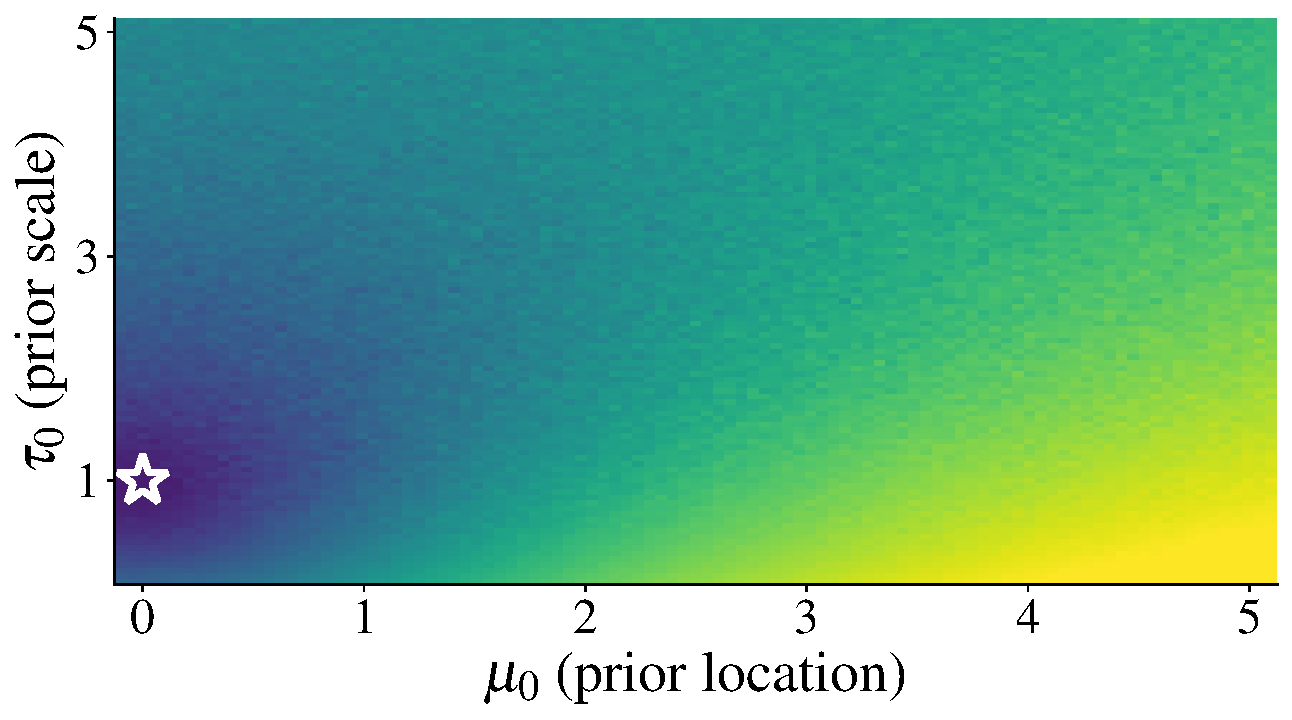
\includegraphics[width=\linewidth]{plots/abf_mvn_means_overcomplete_mmd_grid_prior.pdf}%
%     \end{subfigure}%
%     \hfill%
%     \begin{subfigure}[t]{0.49\linewidth}%
%         \includegraphics[width=\linewidth]{plots/abf_mvn_means_overcomplete_mmd_grid_likelihood_noise.pdf}%
%     \end{subfigure}%    
%     \end{minipage}%
%     \hfill%
%     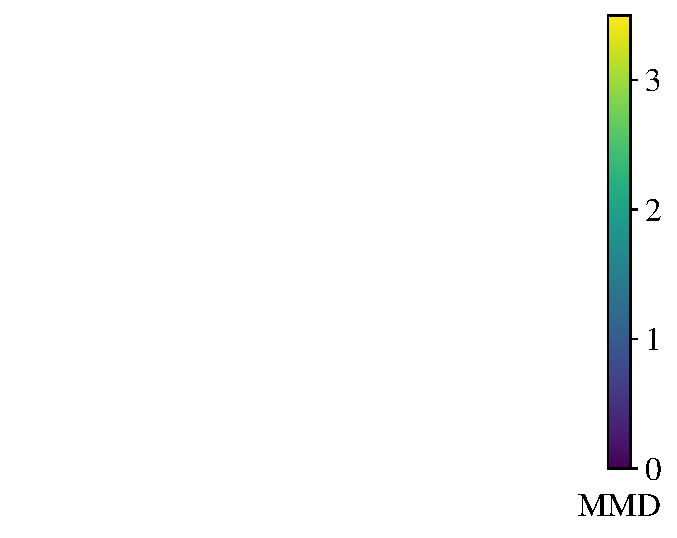
\includegraphics[width=0.09\linewidth, clip, trim=9.5cm 0cm 0.2cm 0cm]{plots/abf_mvn_means_mmd_heatmaps_colorbar.pdf}%
%     \caption{\textbf{Experiment \numberGaussianMeans.} Summary space MMD as a function of misspecification severity. Dashed lines indicate well-specified model configuration (i.e., equal to the training model $\M$).}
%     \label{fig:my_label}
% \end{figure}
\begin{figure}[t]
    \centering
    \begin{subfigure}[t]{.49\textwidth}
     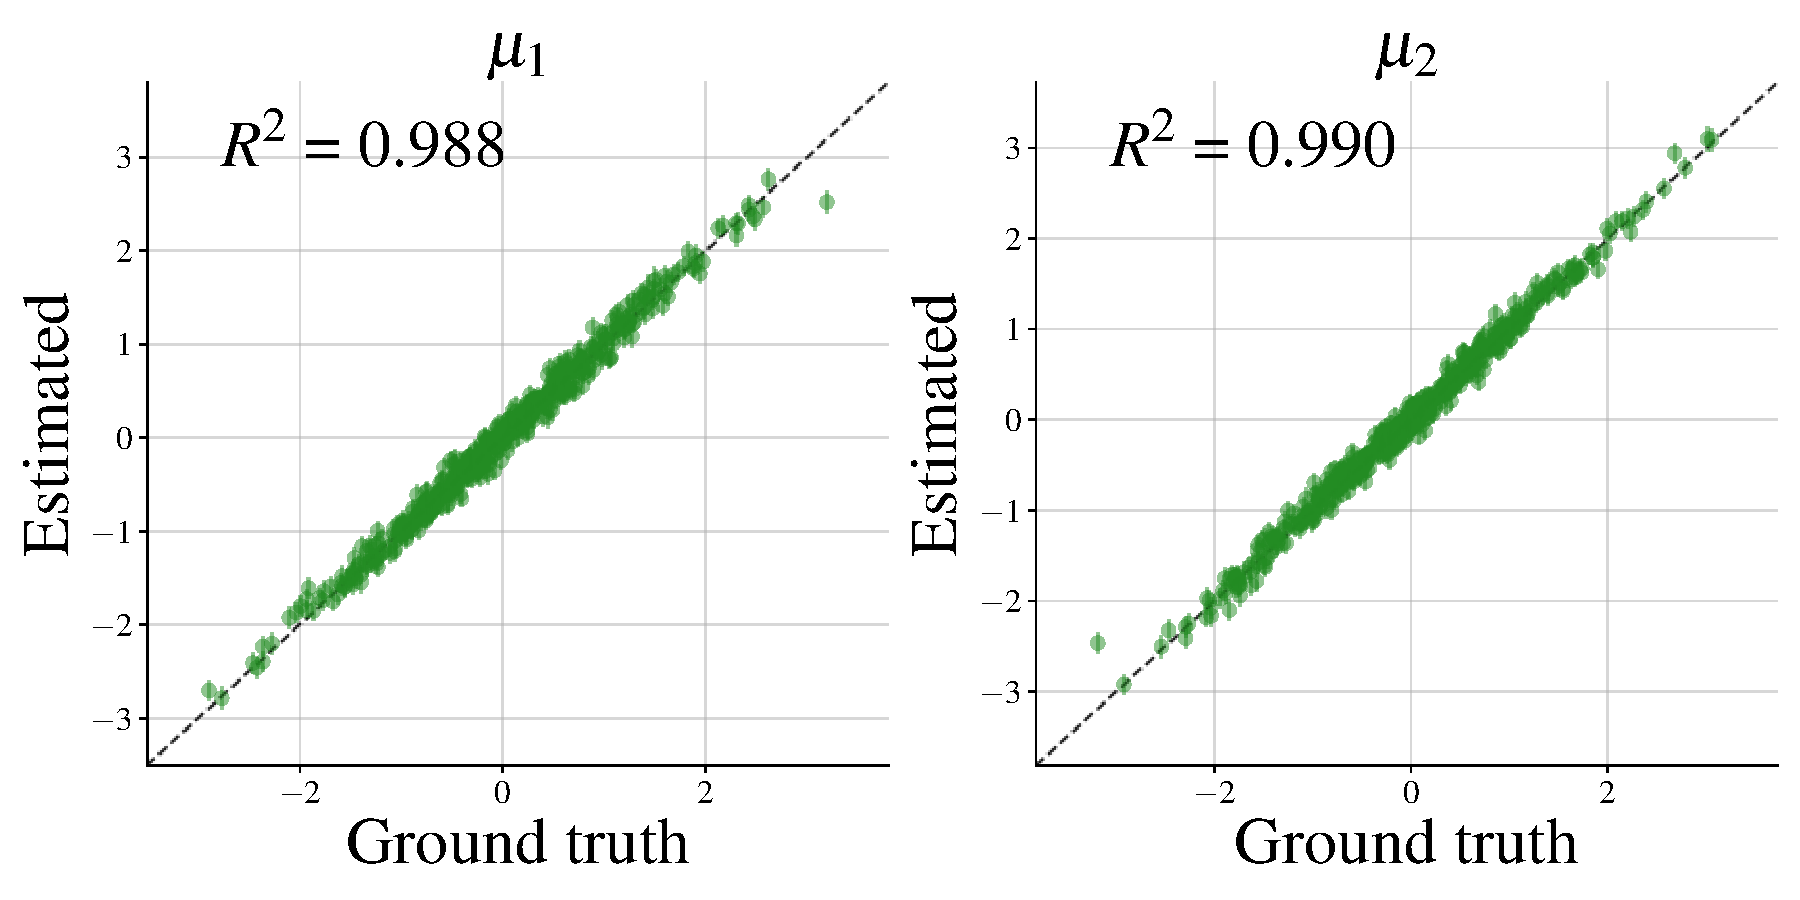
\includegraphics[width=\linewidth]{plots/abf_mvn_means_well_specified_recovery_sufficient.pdf}
     \caption{Excellent parameter recovery.}
     \label{fig:mvn:well-specified-performance:recovery}
    \end{subfigure}
    \hfill
    \begin{subfigure}[t]{.49\textwidth}
     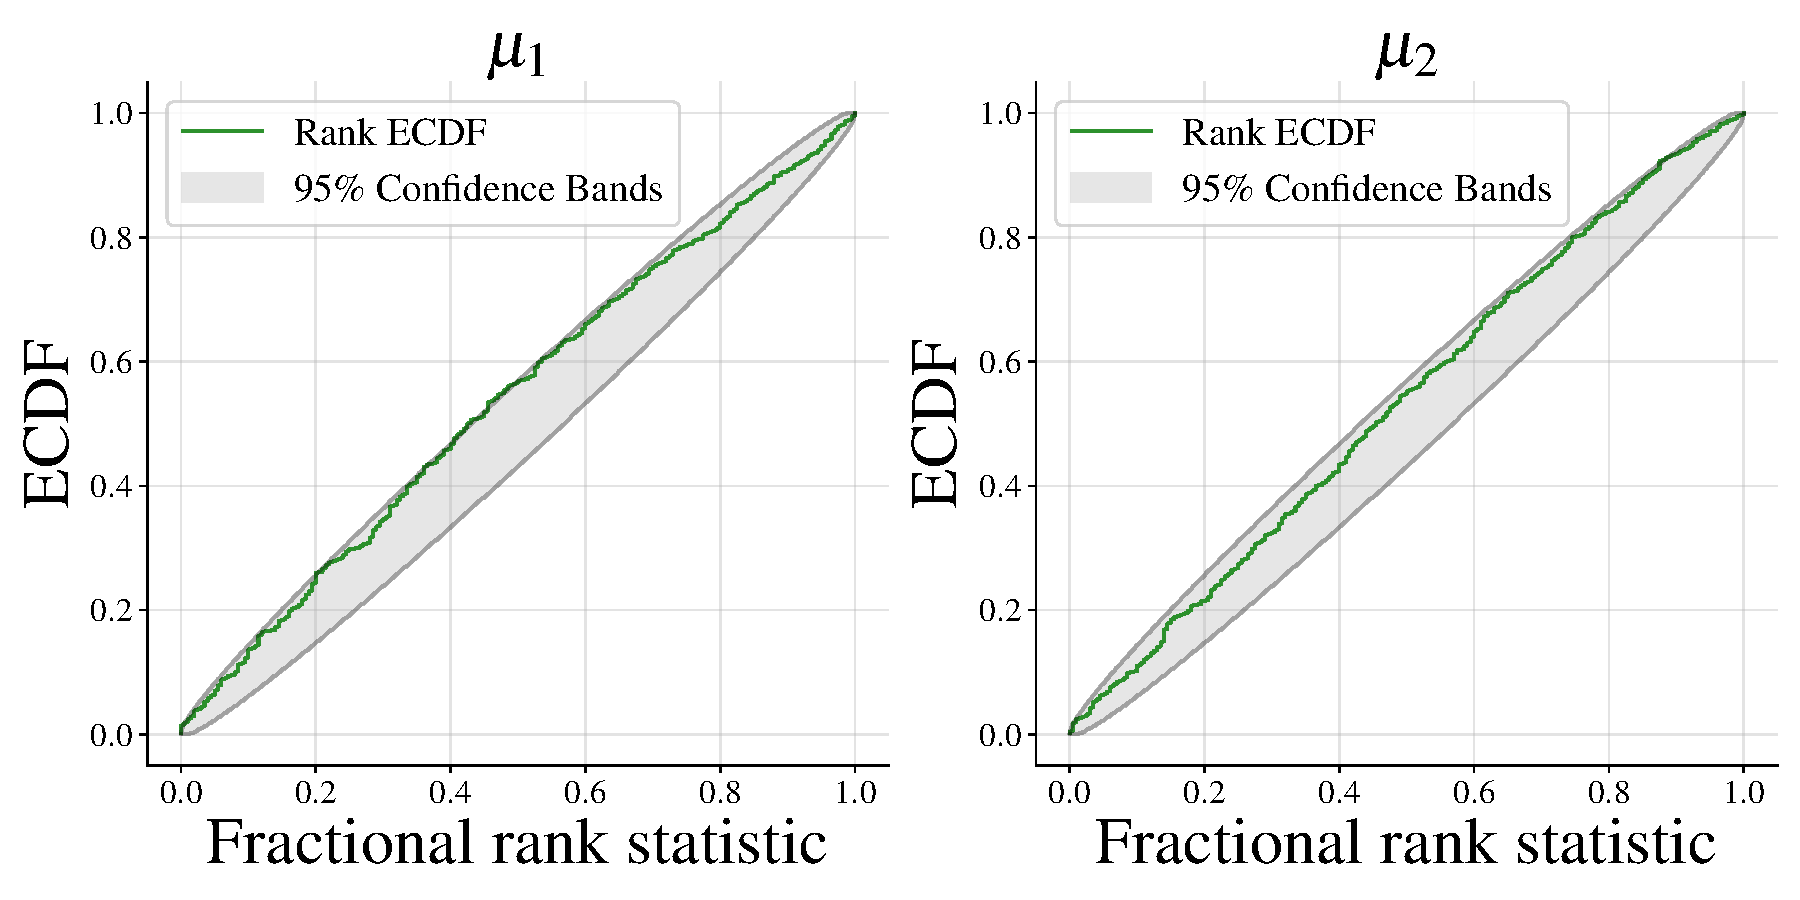
\includegraphics[width=\linewidth]{plots/abf_mvn_means_well_specified_calibration_sufficient.pdf}
     \caption{Excellent calibration.}
     \label{fig:mvn:well-specified-performance:calibration}
    \end{subfigure}
    \caption{\textbf{Experiment \numberGaussianMeans}. When the assumed model is well-specified for the observed data ($\M=\M^*$), both posterior recovery (\subref{fig:mvn:well-specified-performance:recovery}) and calibration (\subref{fig:mvn:well-specified-performance:calibration}) remain excellent with our adjusted optimization objective.}
    \label{fig:mvn:well-specified-performance}
\end{figure}
\subsection{Experiment \numberGaussianMeans: 2D Gaussian Means}\label{sec:experiment-toy-conjugate}
\begin{comment}
\textit{Aims.} Our first proof-of-concept experiment aims to i) demonstrate the utility of our new optimization objective in terms of accurate posterior estimation; ii) highlight the usefulness of MMD for detecting various simulation gaps during inference; iii) investigate the effects of a minimal vs.\ overcomplete summary space with respect to the inference task; and iv) elucidate the relationship between simulation gaps and posterior errors. 
\end{comment}
\begin{table}[b]
\small
    \begin{tabular}{l|ll}
    \centering
        \bfseries Model (MMS) &\bfseries Prior &\bfseries Likelihood\\
        \hline
        $\mathcal{M}$ (No MMS) &
        $\mub\sim\mathcal{N}(\mub_0=\0, \Sigmab_0=\mathbb{I})$&
        $\x_k\sim\mathcal{N}(\mub, \Sigmab=\mathbb{I})$
        \\
        $\mathcal{M}_P$ (Prior) &
        $\mub\sim\mathcal{N}(\mub_0 \neq \0, \Sigmab_0=\tau_0\mathbb{I}), \tau_0\in\mathbb{R}^+$&
        $\x_k\sim\mathcal{N}(\mub, \Sigmab=\mathbb{I})$\\
        $\mathcal{M}_S$ (Simulator) &
        $\mub\sim\mathcal{N}(\mub_0=\0, \Sigmab_0=\mathbb{I})$&
        $\x_k\sim\mathcal{N}(\mub, \Sigmab=\tau\mathbb{I}), \tau\in\mathbb{R}^+$
        \\
        $\mathcal{M}_N$ (Noise)&
        $\mub\sim\mathcal{N}(\mub_0=\0, \Sigmab_0=\mathbb{I})$ & 
        $\x_k\sim\lambda\cdot\mathrm{Beta}(2, 5)+(1-\lambda)\cdot\mathcal{N}(\mub, \Sigmab=\mathbb{I})%, \lambda\in[0, 1]
        $
    \end{tabular}%
    \caption{\textbf{Experiment \numberGaussianMeans.} Investigated model misspecifications.}
    \label{tab:mvn-mean-misspecifications}
\end{table}
We set the stage by estimating the mean of a $2$-dimensional conjugate Gaussian model with $K=100$ observations per data set and a known analytic posterior in order to illustrate our method.
This experiment contains the Gaussian examples from \citet{frazier_model_2020} and \citet{ward_robust_2022}, and extends them by (i) studying misspecifications beyond the likelihood variance (see below); and (ii) implementing continuously widening simulation gaps, as opposed to a single discrete misspecification.
The data generating process is defined as
\begin{equation}
    \x_k \sim \mathcal{N}(\x\given\mub, \Sigmab) \quad\text{for } k = 1,...,K\qquad \text{with }\;\;
    \mub \sim \mathcal{N}(\mub\given\mub_0, \Sigmab_0).
\end{equation}
We use a permutation invariant summary network \cite{invariant} with $S=2$ output dimensions, which equal the number of minimal sufficient statistics\footnote{The terms ``minimal'', ``sufficient'', and ``overcomplete'' refer to the inference task and \emph{not} to the data. Thus, $S=2$ summary statistics are \emph{sufficient} to solve the inference task, namely recover two means.} implied by the analytic posterior.
For training the posterior approximator, we set the prior of the generative model $\M$ to a unit Gaussian and the likelihood covariance $\Sigmab$ to an identity matrix.
The induced misspecifications during test time are outlined in \autoref{tab:mvn-mean-misspecifications}.\footnote{Note that Experiment \numberGaussianMeans~from \citet{ward_robust_2022} is represented by the scenario $\mathcal{M}_S$ with $\tau=2$.
In addition, we study model misspecification across the entire plausible parameter space of the likelihood variance, as well as prior ($\M_P$) and noise ($\M_N$) misspecification.
}
We conduct the experiment with BayesFlow and SNPE-C, both equipped with our adjusted optimization objective.%
%\footnote{BayesFlow is available at \url{https://github.com/stefanradev93/BayesFlow} (MIT license), \\SNPE-C is available in the sbi packge at \url{https://github.com/mackelab/sbi} (AGPL-3.0 license).}
%\footnotesize{$^a$ A sample from the noise model $\mathcal{M}_N$ is simulated by randomly choosing a fraction $\lambda\in[0,1]$ of the Gaussian data $\x$ and replacing it with samples from $\etab\sim\mathrm{Beta}(2, 5)$ which is rescaled to $\pm3\sigma_{\x}$ in order to match the empirical scale and make the detection task harder.}
%\textit{Results.} 
% \begin{figure}
%     \centering
%     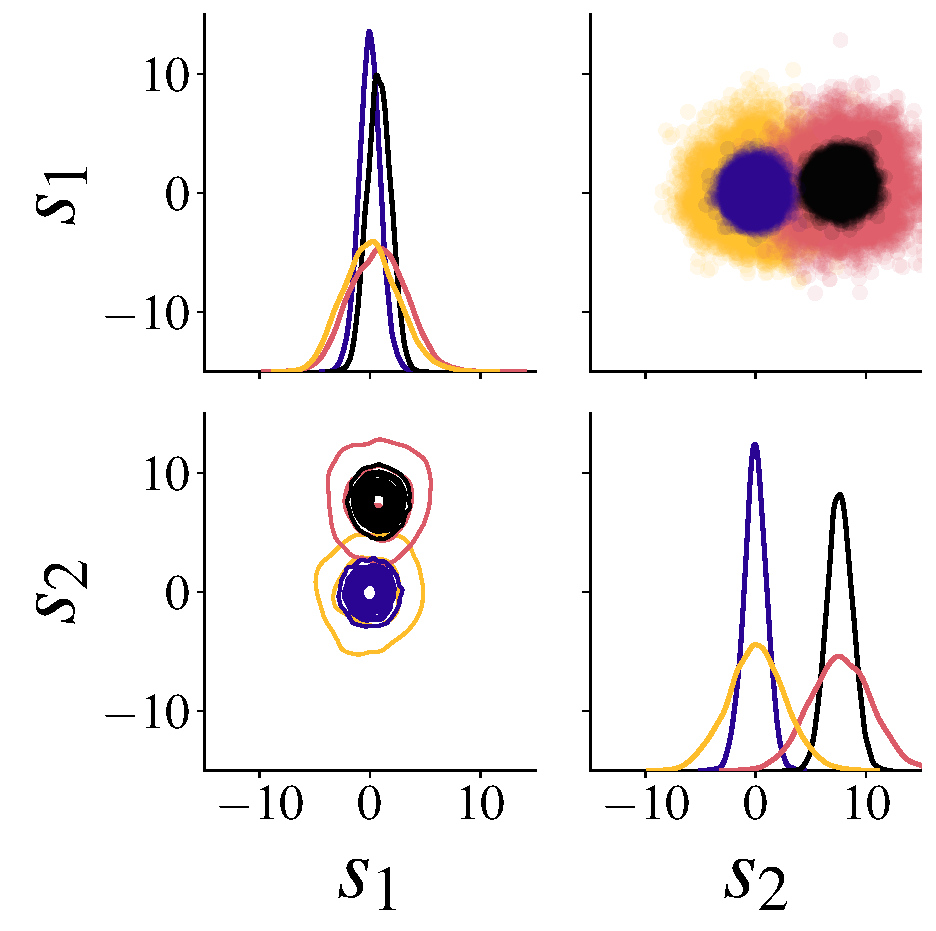
\includegraphics[width=.35\linewidth]{abf_mvn_means_sufficient_pairplot.pdf}
%     \hfill
%     \includegraphics[width=.58\linewidth]{abf_mvn_means_sufficient_mmd_grid_prior.pdf}\\
%     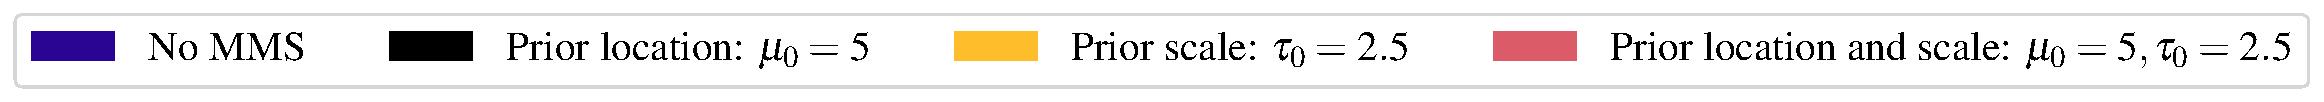
\includegraphics[width=\linewidth]{abf_mvn_means_sufficient_pairplot_MMD_legend.pdf}
%     \caption{\textbf{Experiment \numberGaussianMeans.} Prior misspecification can be detected with a minimal sufficient summary network ($S=2$).
%     \textbf{Left:} All prior misspecifications are distinguishable from the typical summary space (blue).
%     \textbf{Right:} MMD increases as the simulation gap worsens.}
%     \label{fig:exp:mvn-means:sufficient:prior-MMS}
% \end{figure}
\begin{figure}[t]
    \centering
    \begin{subfigure}[t]{0.45\linewidth}
        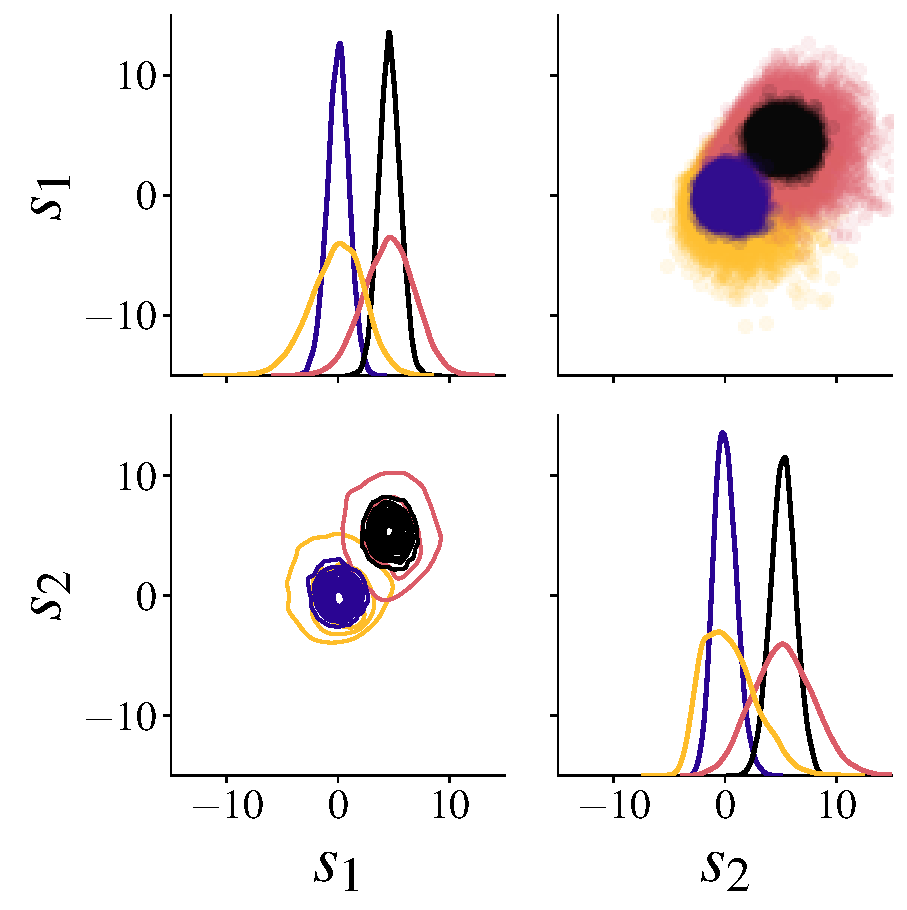
\includegraphics[width=\linewidth]{plots/abf_mvn_means_sufficient_pairplot_new.pdf}
    \end{subfigure}\hfill
    \begin{subfigure}[t]{0.45\linewidth}
        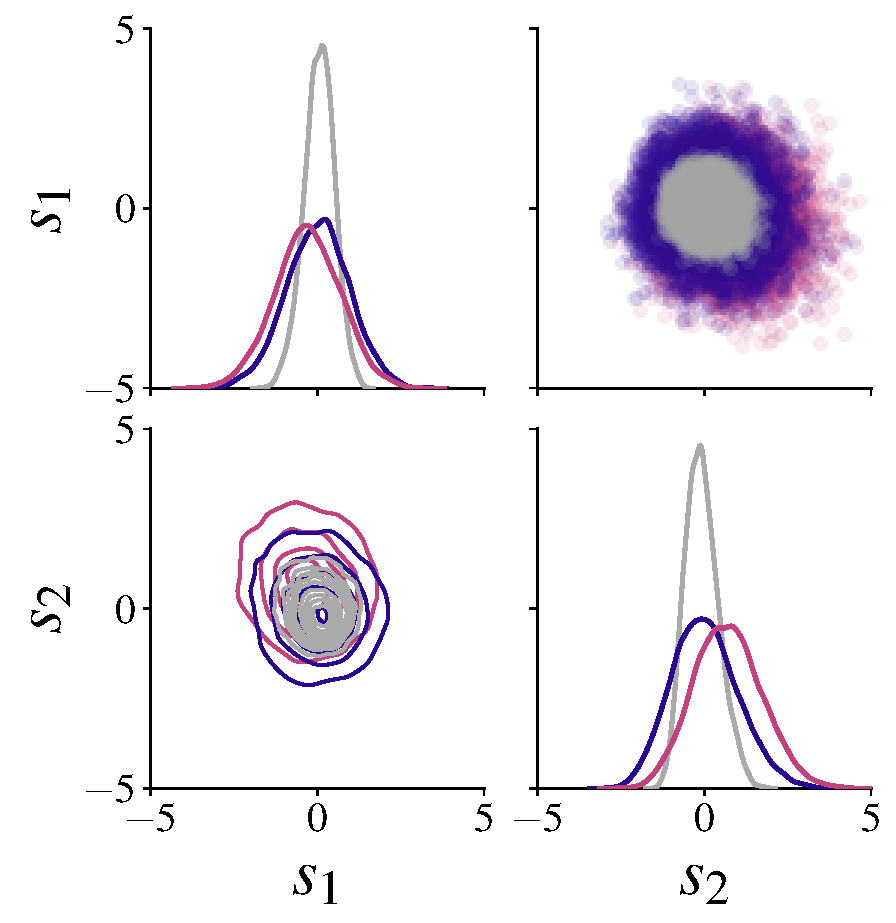
\includegraphics[width=\linewidth]{plots/abf_mvn_means_sufficient_simulator_noise_pairplot_new.pdf}
    \end{subfigure}\\
    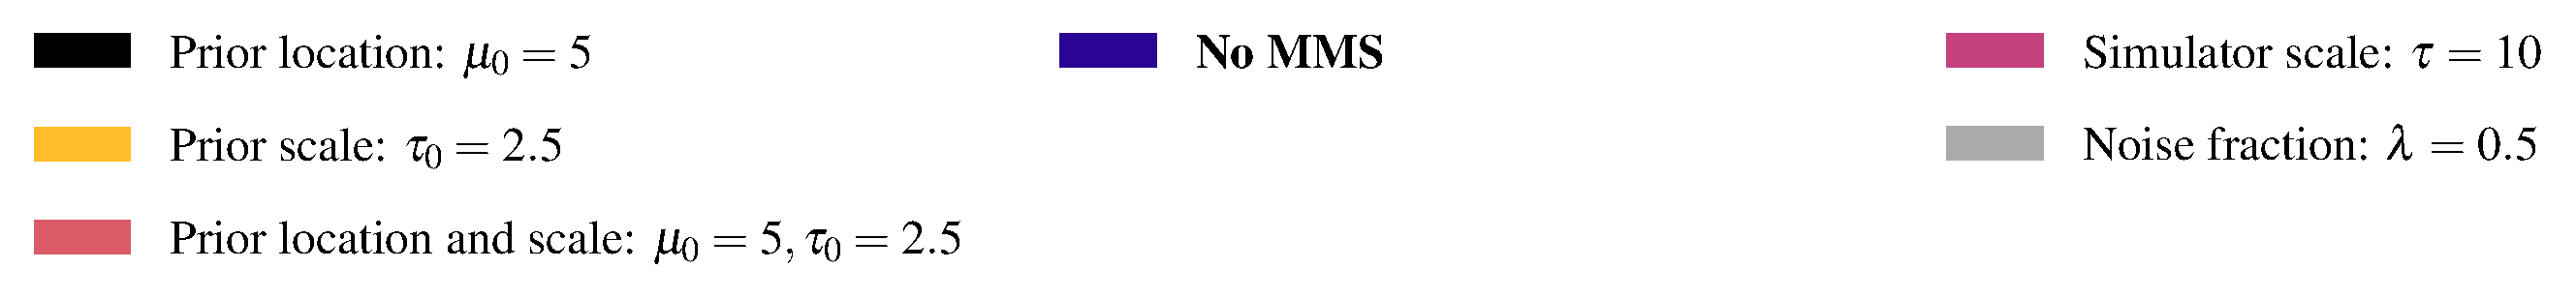
\includegraphics[width=0.95\linewidth]{plots/abf_mvn_means_sufficient_pairplot_MMD_legend_new.pdf}
    \caption{\textbf{Experiment \numberGaussianMeans.} Summary space samples for the minimal sufficient summary network ($S=2$) from a well-specified model $\M$ (blue) and several misspecified configurations. \textbf{Left:} Prior misspecification can be detected. \textbf{Right:} Noise misspecification can be detected, while simulator scale misspecification is indistinguishable from the validation summary statistics (but see results for $S=4$).}
    \label{fig:mvn:pairplot}
\end{figure}

\textit{Results.}
The BayesFlow network trained to minimize the augmented objective (Eq.~\ref{eq:bf_kl_mmd}) exhibits excellent recovery of the analytic posterior means when no misspecification is present (see \autoref{fig:mvn:well-specified-performance:recovery}). % (30min training time on a CPU). % (see \autoref{fig:app:mvn:performance}).
Furthermore, the posterior calibration \citep[SBC;][]{talts_validating_2020} remains excellent, as shown in \autoref{fig:mvn:well-specified-performance:calibration} via simultaneous confidence bands of rank ECDFs \cite{sailynoja_graphical_2021}.
All prior misspecifications manifest themselves in anomalies in the summary space which are directly detectable through visual inspection of the $2$-dimensional summary space in \autoref{fig:mvn:pairplot} (left). 
Note that the combined prior misspecification (location and scale) exhibits a summary space pattern that combines the location and scale of the respective location and scale misspecifications.
However, based on the $2$-dimensional summary space, misspecifications in the fixed parameters of the likelihood ($\tau$) and mixture noise are not detectable via an increased MMD (see \autoref{fig:mvn:mmd}, top right).
\begin{figure}[t]
    \centering
    \begin{subfigure}[c]{0.9\linewidth}%
    \setlength\tabcolsep{2pt}%
    \begin{tabular}{ccccc}
    && \multicolumn{2}{c}{\textbf{Model Misspecification}} & \\
        & &
        \textbf{Prior} ($\M_P$) &
        \textbf{Simulator} ($\M_S$) \textbf{\& noise} ($\M_N$)
        \\
        \multirow{2}{*}{\hspace*{-0.1cm}\rotatebox[origin=c]{90}{\textbf{Summary Network}}} &
        \rotatebox[origin=c]{90}{\textbf{minimal}} &
        \raisebox{-0.48\height}{\includegraphics[width=0.45\linewidth]{plots/abf_mvn_means_sufficient_mmd_grid_prior.pdf}} &
        \raisebox{-0.48\height}{\includegraphics[width=0.46\linewidth]{plots/abf_mvn_means_sufficient_mmd_grid_likelihood_noise.pdf}}
        \\
        &\rotatebox[origin=c]{90}{\textbf{overcomplete}} &
        \raisebox{-0.5\height}{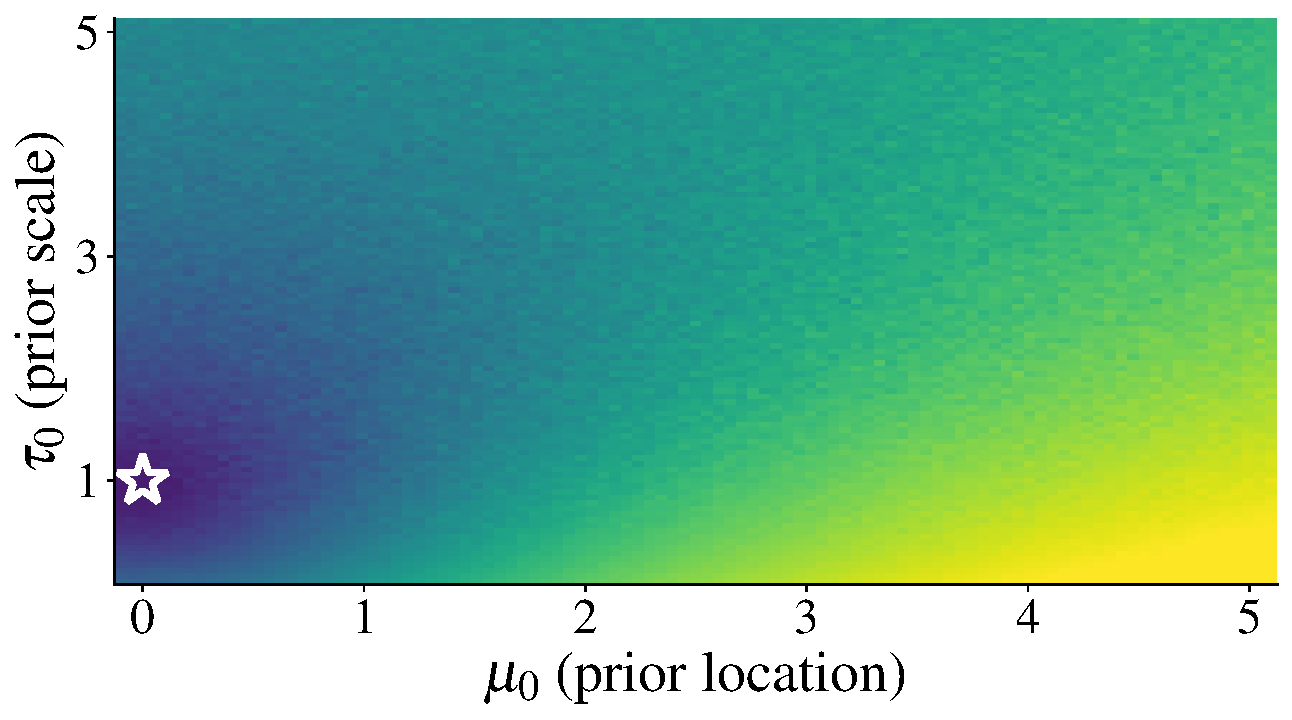
\includegraphics[width=0.45\linewidth]{plots/abf_mvn_means_overcomplete_mmd_grid_prior.pdf}} &
        \raisebox{-0.5\height}{\includegraphics[width=0.46\linewidth]{plots/abf_mvn_means_overcomplete_mmd_grid_likelihood_noise.pdf}}
    \end{tabular}% 
    \end{subfigure}%
    \begin{subfigure}[c]{0.06\linewidth}
    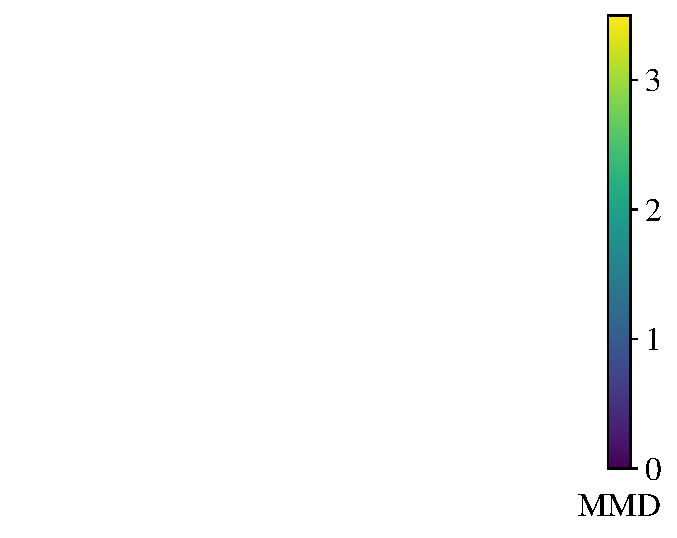
\includegraphics[width=\linewidth, clip, trim=9.8cm 0cm 0.2cm 0cm]{plots/abf_mvn_means_mmd_heatmaps_colorbar.pdf}
    \end{subfigure}
    \caption{\textbf{Experiment \numberGaussianMeans.} Summary space MMD as a function of misspecification severity. White stars indicate the well-specified model configuration (i.e., equal to the training model $\M$).}
    \label{fig:mvn:mmd}
\end{figure}

We further investigate the effect of an \emph{overcomplete} summary space with respect to the inference task, namely $S=4$ learned summary statistics with an otherwise equal architecture.
In addition to prior misspecifications, the overcomplete summary network also captures misspecifications in the noise and simulator via the MMD criterion (see \autoref{fig:mvn:mmd}, bottom row).
Furthermore, the induced misspecifications in the noise and simulator are visually detectable in the summary space samples (see \autoref{fig:app:mvn-means:overcomplete:pairplot} in the Appendix).
Recall that the $2$-dimensional summary space fails to capture these misspecifications (see \autoref{fig:mvn:mmd}, top right).
% \begin{figure}
% \centering
%     \begin{minipage}{.44\linewidth}
%         \includegraphics[width=\linewidth]{abf_mvn_means_sufficient_mmd_grid_likelihood_noise.pdf}
%     \end{minipage}
%     \hfill
%     \begin{minipage}{.44\linewidth}
%         \includegraphics[width=\linewidth]{abf_mvn_means_overcomplete_mmd_grid_likelihood_noise.pdf}
%     \end{minipage}
    
%     \begin{minipage}{.60\linewidth}
%         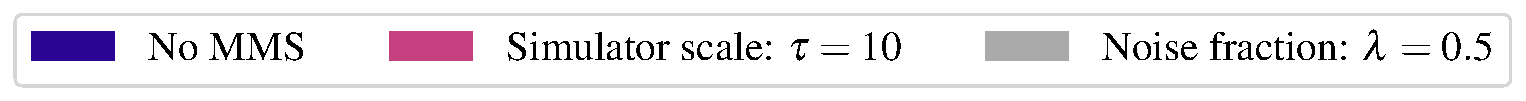
\includegraphics[width=\linewidth]{abf_mvn_means_overcomplete_pairplot_MMD_legend.pdf}
%     \end{minipage}
    
%     \begin{minipage}{.48\linewidth}
%         \begin{subfigure}[t]{\linewidth}
%             \caption{Minimal sufficient statistics: no MMS detection.}
%             \label{fig:exp:mvn-means:mmd-grid:sufficient}
%         \end{subfigure}
%     \end{minipage}
%     \hfill
%     \begin{minipage}{.48\linewidth}
%         \begin{subfigure}[t]{\linewidth}
%             \caption{Overcomplete sufficient statistics: MMS detection possible.}
%             \label{fig:exp:mvn-means:mmd-grid:overcomplete}
%         \end{subfigure}
%     \end{minipage}
%     \caption{\textbf{Experiment \numberGaussianMeans.} MMD as a function of simulator and noise misspecification. While the minimal summary network yields essentially equal MMDs across the grid, the overcomplete summary network captures model misspecification in both simulator and noise.}
%     \label{fig:exp:mvn-means:mmd-grid}
% \end{figure}
% \begin{figure}
%         \begin{subfigure}[t]{.48\linewidth}
%             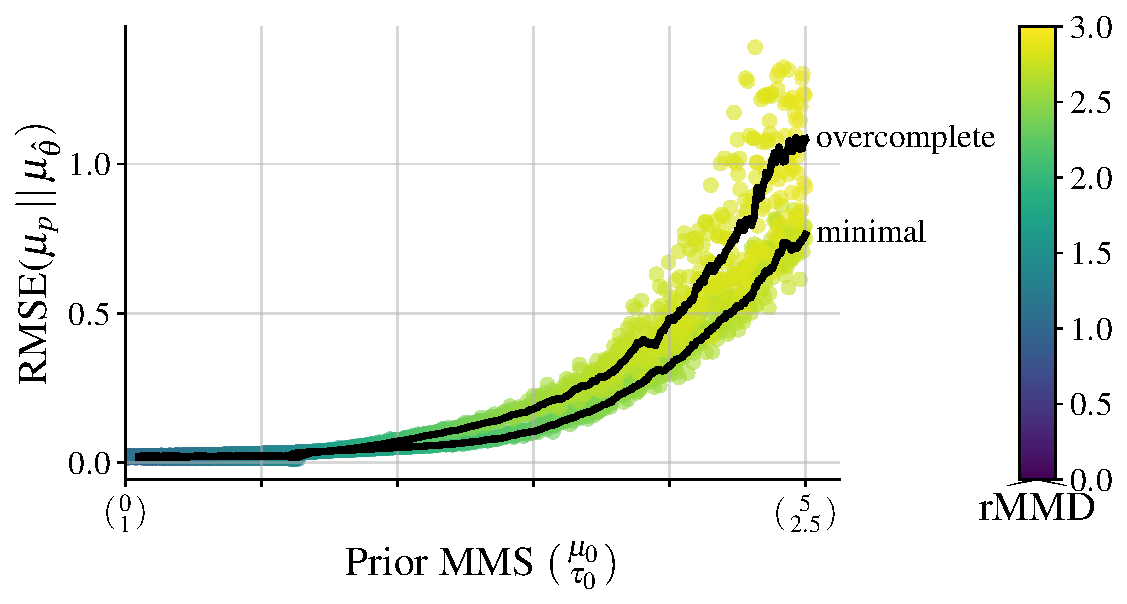
\includegraphics[width=\linewidth]{abf_mvn_means_sufficient_vs_overcomplete_MMD_Error_Prior.pdf}
%             \caption{Prior misspecification:
%             %$\vectwo{\mu_0}{\tau_0} = \vectwo{0}{1} \ldots \vectwo{5}{2.5}$,
%             Both summary networks (minimal and overcomplete) detect increasingly severe misspecification through an elevated MMD and lead to a higher posterior error (RMSE) of the inference network.}            \label{fig:exp:mvn-means:MMD-error:prior}
%         \end{subfigure}
%     \hfill
%         \begin{subfigure}[t]{.48\linewidth}
%             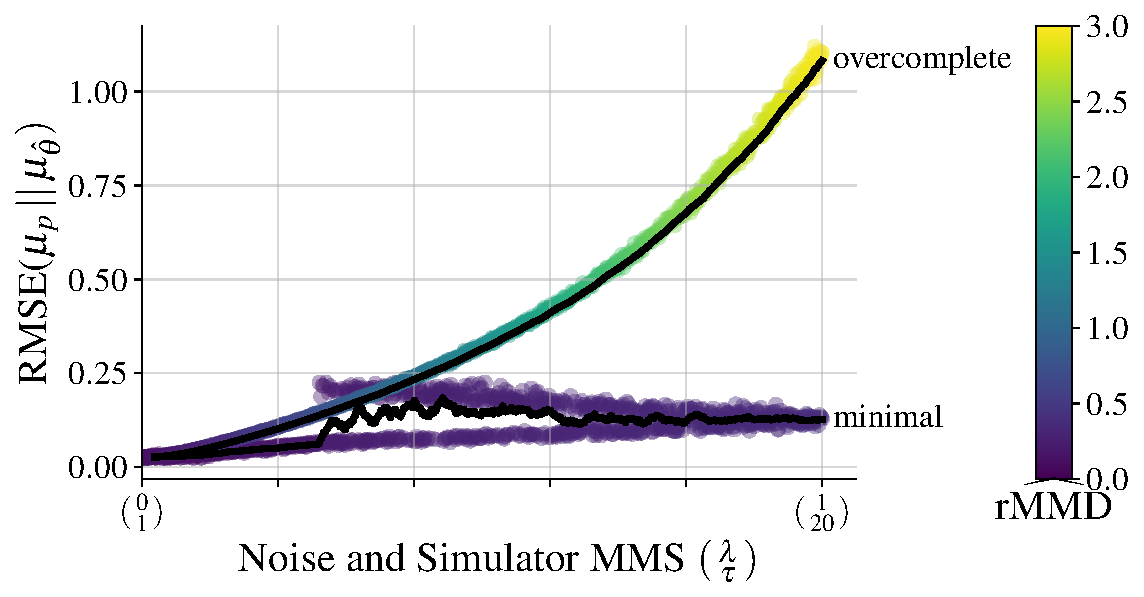
\includegraphics[width=\linewidth]{abf_mvn_means_sufficient_vs_overcomplete_MMD_Error_Noise_Likelihood.pdf}
%             \caption{Noise and simulator misspecification:
%             %$\vectwo{\lambda}{\tau} = \vectwo{0}{1} \dots \vectwo{1}{20}$,
%             While the minimal network exhibits poor detection, its posterior recovery is not impaired either. The overcomplete network captures increasingly severe misspecification but suffers from an increased posterior error (RMSE).
%             }
%             \label{fig:exp:mvn-means:MMD-error:likelihood-noise}
%         \end{subfigure}
% \caption{\textbf{Experiment \numberGaussianMeans.} Posterior error (RMSE between analytic posterior means $\mub_p$ and approximate posterior means $\mub_{\widehat{\thetab}}$) as a function of model misspecification severity, as indexed by the MMD criterion. }
% \label{fig:exp:mvn-means:MMD-error}
% \end{figure}

%Finally, we compute the error in posterior recovery as a function of the misspecification severity. To ease visualization, the posterior error $\varepsilon_n$ for each data set with index $n=1,\ldots, N$ is defined as the difference in the first moment: We compute the expected value of the analytic posterior $\mathbb{E}_{p(\thetab \given \x^{(n)}, \M)}[\thetab]$ and the average of the $L$ draws from the approximate posterior $\frac{1}{L}\sum_{l=1}^L\thetab^{(l, n)}$. Subsequently, we compute the RMSE over $N$ data sets as $\sqrt{\sum_{n=1}^N\varepsilon_n^2}$ and analyze the connection between model misspecification and RMSE in the following.
\begin{figure}[t]
\centering
    \begin{subfigure}[c]{0.9\linewidth}%
    \setlength\tabcolsep{2pt}%
    \begin{tabular}{ccccc}
    && \multicolumn{2}{c}{\textbf{Model Misspecification}} & \\
        & &
        \textbf{Prior} ($\M_P$) &
        \textbf{Simulator} ($\M_S$) \textbf{\& noise} ($\M_N$)
        \\
        \multirow{2}{*}{\hspace*{-0.1cm}\rotatebox[origin=c]{90}{\textbf{Summary Network}}} &
        \rotatebox[origin=c]{90}{\textbf{minimal}} &
        \raisebox{-0.48\height}{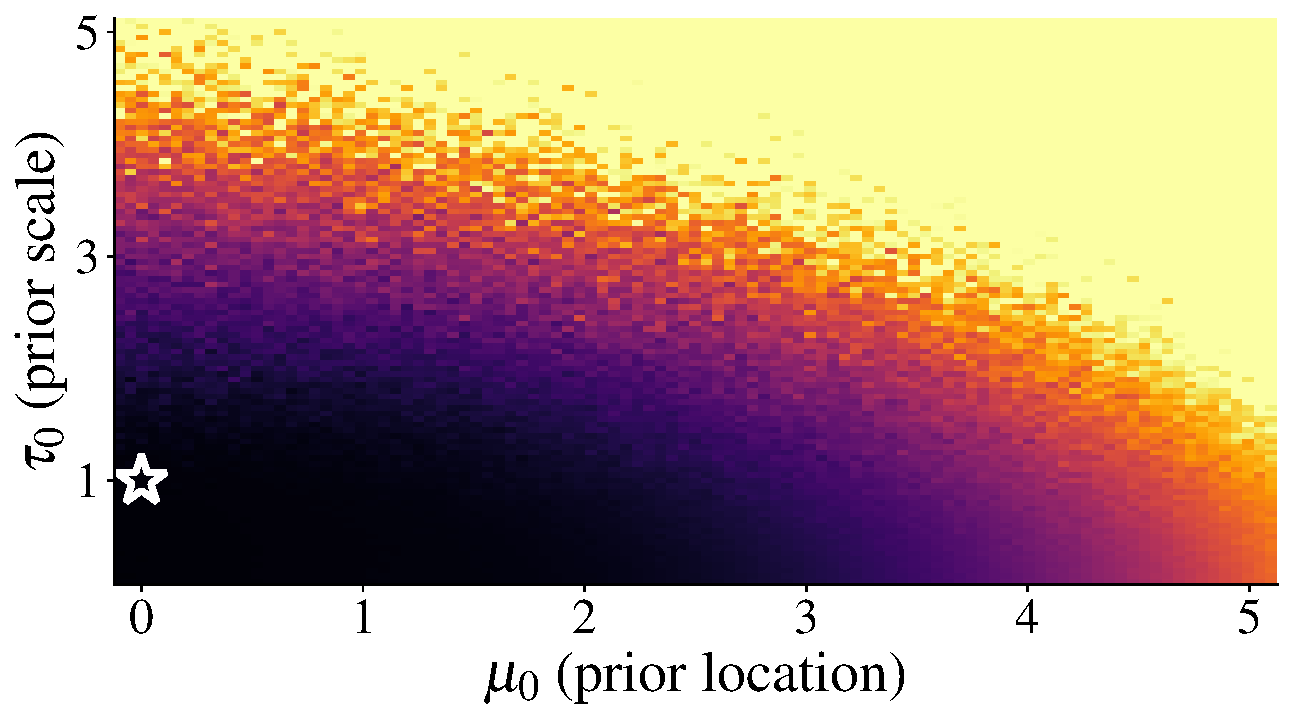
\includegraphics[width=0.45\linewidth]{plots/abf_mvn_means_sufficient_rmse_grid_prior.pdf}} &
        \raisebox{-0.48\height}{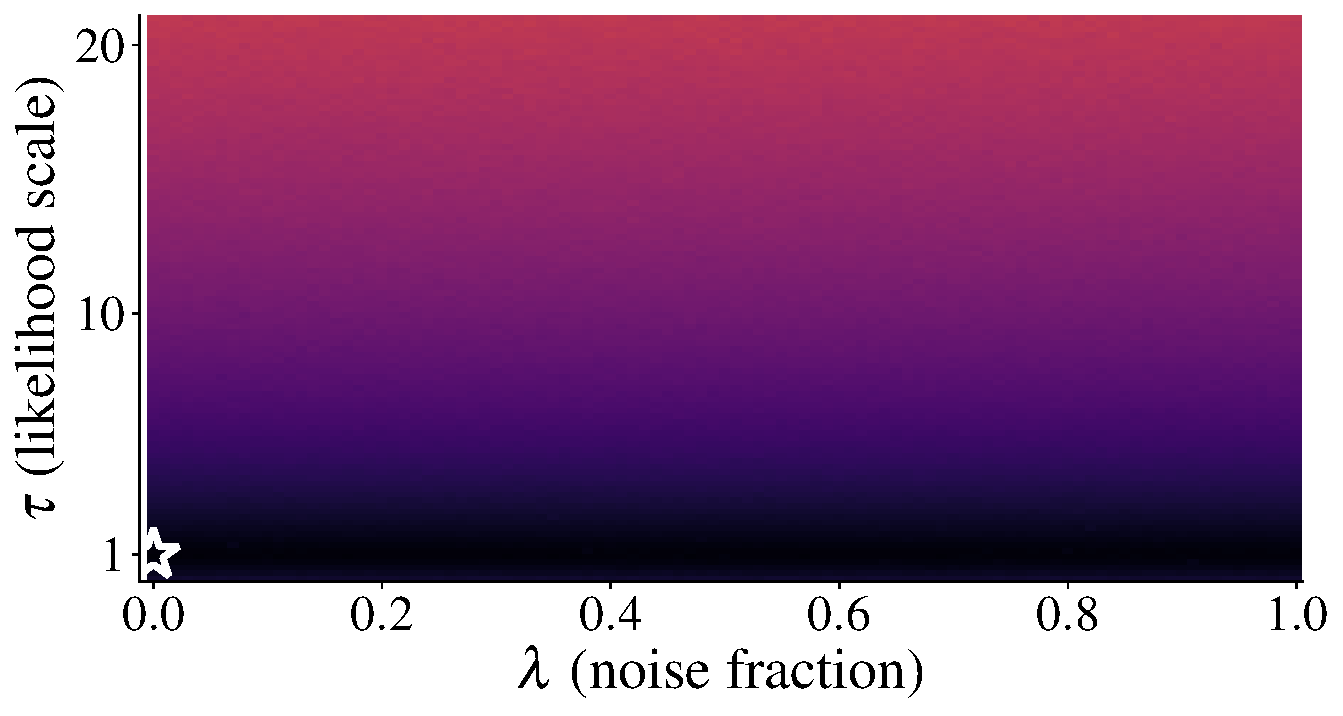
\includegraphics[width=0.46\linewidth]{plots/abf_mvn_means_sufficient_rmse_grid_simulator_noise.pdf}}
        \\
        &\rotatebox[origin=c]{90}{\textbf{overcomplete}} &
        \raisebox{-0.5\height}{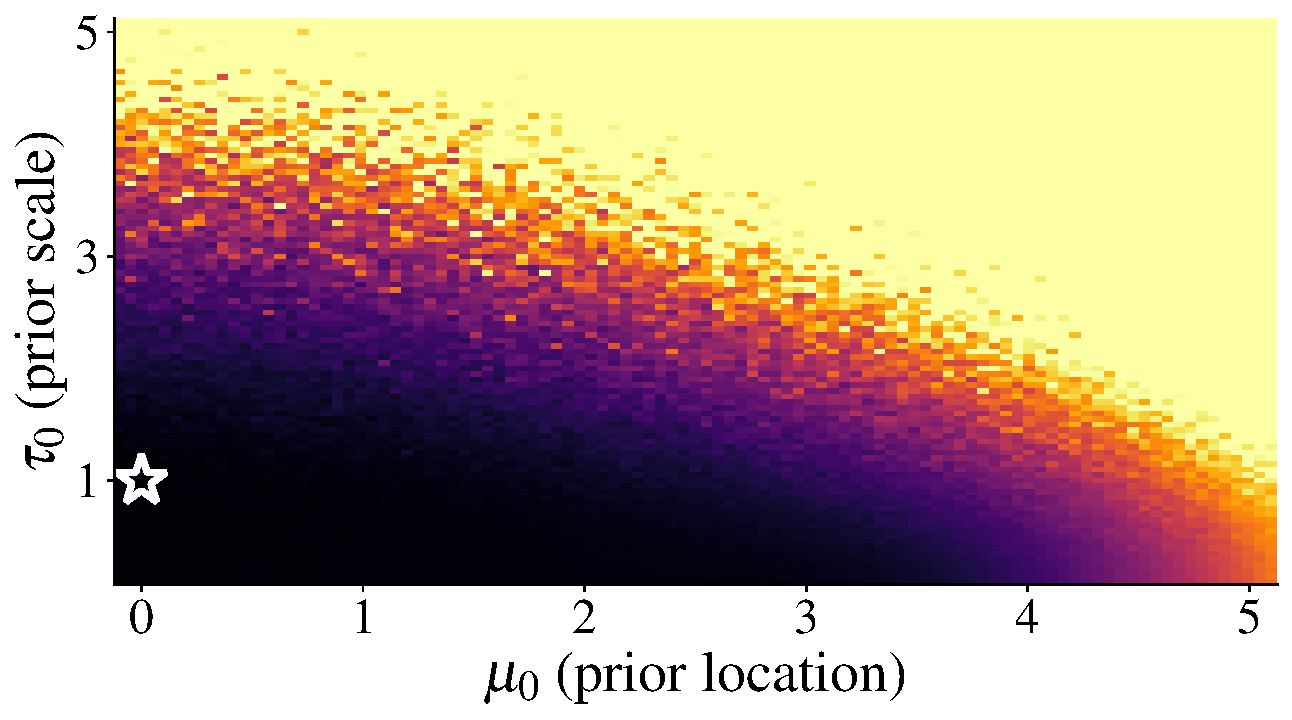
\includegraphics[width=0.45\linewidth]{plots/abf_mvn_means_overcomplete_rmse_grid_prior.pdf}} &
        \raisebox{-0.5\height}{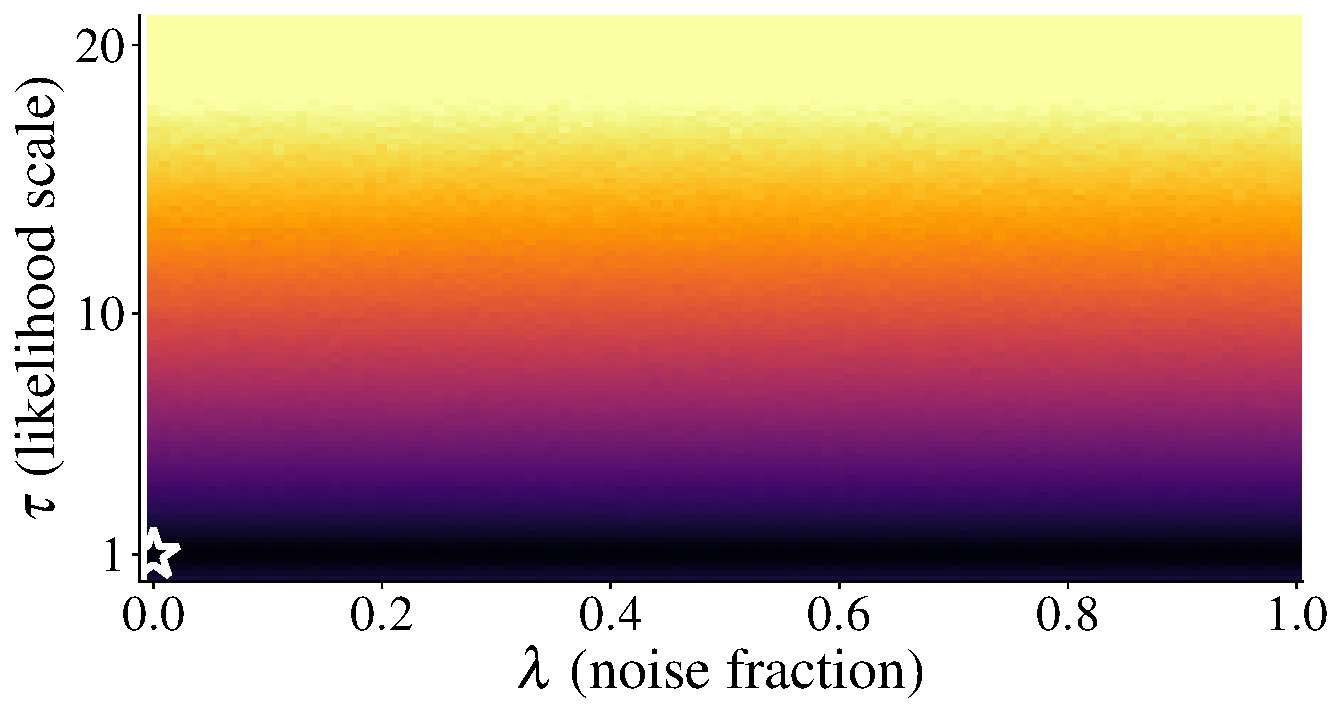
\includegraphics[width=0.46\linewidth]{plots/abf_mvn_means_overcomplete_rmse_grid_simulator_noise.pdf}}
    \end{tabular}% 
    \end{subfigure}%
    \begin{subfigure}[c]{0.08\linewidth}
    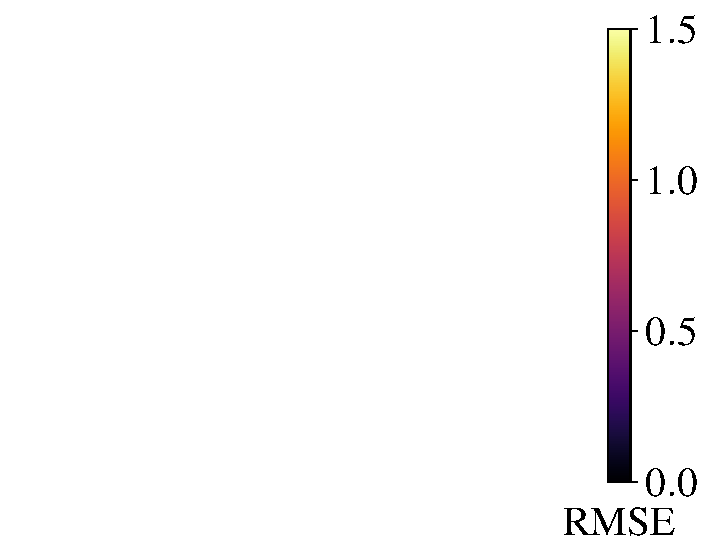
\includegraphics[width=\linewidth, clip, trim=9.5cm 0cm 0.2cm 0cm]{plots/abf_mvn_means_rmse_heatmaps_colorbar.pdf}%        
    \end{subfigure}
    \caption{\textbf{Experiment \numberGaussianMeans.} Posterior Error (RMSE of correct vs.\ analytic posterior means) as a function of misspecification severity. White stars indicate the well-specified model configuration (i.e., equal to the training model $\M$).}
    \label{fig:mvn:rmse}
\end{figure}
Finally, we compute the error in posterior recovery as a function of the misspecification severity.
To ease visualization, we use the RMSE of the approximated posterior mean from $L$ samples $\hat{\overline{\thetab}}^{(n)} = \frac{1}{L}\sum_{l=1}^L\thetab^{(l, n)}$ against the analytic posterior mean $\overline{\thetab}^{(n)}$ across a number of $N$ data sets.\footnote{Since the approximate posterior in the Gaussian model is likely to be symmetric---and the analytic posterior is symmetric by definition---we deem the posterior mean as an appropriate evaluation target for the RMSE across data sets.
In fact, error metrics over several posterior quantiles (\ie, $Q_{25}$, $Q_{50}$ and $Q_{75}$) in the place of posterior means yield identical results.
Other common metrics (\ie, MSE and MAE) yield identical results.}
% indexed by $n$: $\text{RMSE} = \sqrt{\sum_{n=1}^N (\hat{\overline{\thetab}}^{(n)} - \overline{\thetab}^{(n)})^2}.$ 
% \begin{equation}
%     \mathrm{RMSE} = \sum\limits_{n=1}^N 
%     \Big(
%     \underbrace{\mathbb{E}_{p(\thetab\given\x,\M)}(\thetab)}_{\text{Analytic posterior expectation}}
%     -
%     \underbrace{\big(L^{-1}\sum\limits_{l=1}^L\thetab^{(l)}\big)}_{\text{Approximate posterior mean}}
%     \Big)^2
% \end{equation}

\autoref{fig:mvn:rmse} illustrates that more severe model misspecifications generally coincide with a larger error in posterior estimation across all model misspecifications for both $S=2$ and $S=4$ learned summary statistics, albeit with fundamental differences, as explained in the following.
When processing data emerging from models with misspecified noise and simulator (see \autoref{fig:mvn:rmse}, right column), minimal and overcomplete summary networks exhibit a drastically different behavior:
While the minimal summary network cannot detect noise or simulator simulation gaps, its posterior estimation performance is not heavily impaired either (see \autoref{fig:mvn:rmse}, top right).
On the other hand, the overcomplete summary network is able to capture noise and simulator misspecifications, but also incurs larger posterior inference error (see \autoref{fig:mvn:rmse}, bottom right).
This might suggest a trade-off between model misspecification detection and posterior inference error, depending on the number of learnable summary statistics.

From a practical modeling perspective, researchers might wonder how to choose the number of learnable summary statistics.
While an intuitive heuristic might suggest ``the more, the merrier'', the observed results in this experiment beg to differ depending on the modeling goals.
If the focus in a critical application lies in detecting potential simulation gaps, it might be advantageous to utilize a large (overcomplete) summary vector.
However, modelers might also desire a network which is as robust as possible during test time, opting for a smaller number of summary statistics.
\textbf{Experiments \numberCovid} addresses this question for a complex non-linear time series model where the number of sufficient summary statistics is unknown.

\textit{SNPE-C (APT).}
Our method successfully detects model misspecification using SNPE-C \cite{apt} with the proposed MMD criterion and a structured summary space (see \autoref{app:snpe}).
The results are largely equivalent to those obtained with BayesFlow \cite{bayesflow}.
The nuanced differences are not soundly interpretable due to the architectural differences of the two frameworks.

\subsection{Experiment \numberGaussianMeansCov: 5D Gaussian Means and Covariance}
\begin{figure}[t]
    \begin{minipage}{.48\linewidth}
        \begin{subfigure}[t]{\linewidth}
            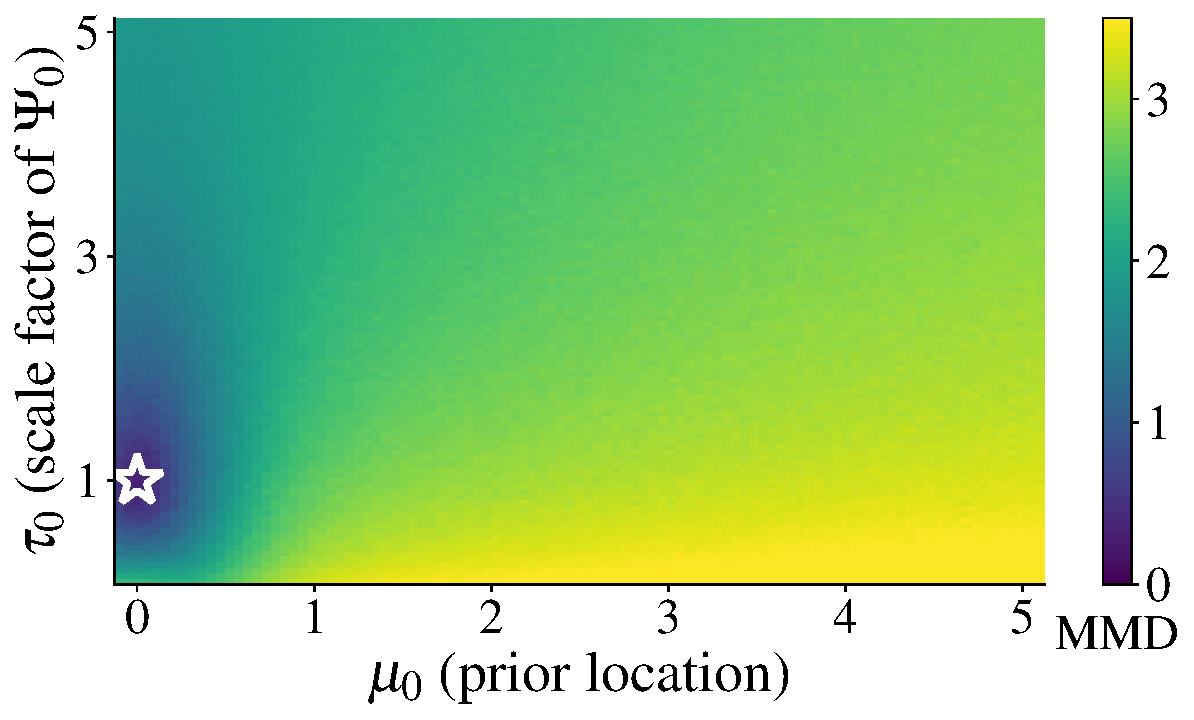
\includegraphics[width=\linewidth]{plots/abf_mvn_full_mmd_grid_prior.pdf}
            \caption{Prior misspecification.}
            \label{fig:app:mvn-full:MMD:prior}
        \end{subfigure}
    \end{minipage}
    \hfill
    \begin{minipage}{.48\linewidth}
        \begin{subfigure}[t]{\linewidth}
            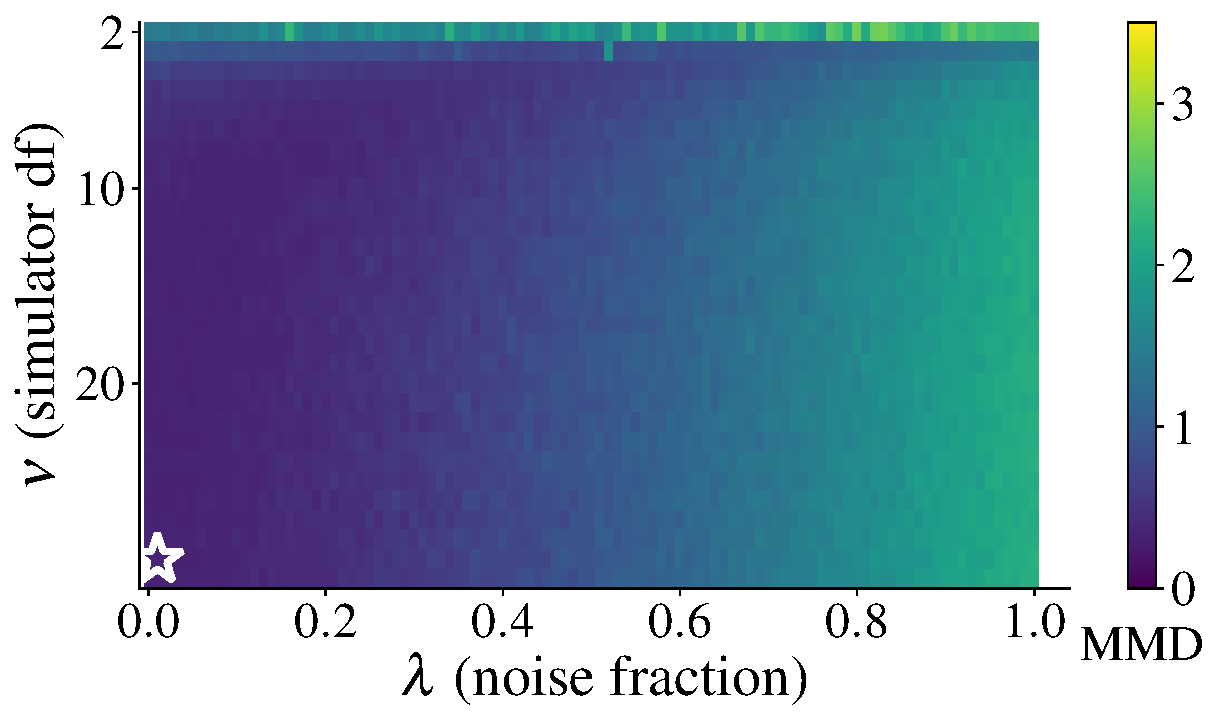
\includegraphics[width=\linewidth]{plots/abf_mvn_full_mmd_grid_likelihood_noise.pdf}
            \caption{Simulator and noise misspecification.}
            \label{fig:app:mvn-full:MMD:likelihood-noise}
        \end{subfigure}
    \end{minipage}
    \hspace*{1cm}
\caption{\textbf{Experiment \numberGaussianMeansCov.} MMD as a function of model misspecification severity in the prior (left) as well as simulator and noise (right). 
All induced model misspecifications are detectable through an increased MMD.
White stars represent the configuration for the well-specified model (i.e., training model $\M$).
The deviating pattern in the top-most row of (\subref{fig:app:mvn-full:MMD:likelihood-noise}) is caused by the infinite variance of the Student $t$ likelihood with $\nu=2$ degrees of freedom: This is an extreme simulation gap with respect to the unit Gaussian model~$\M$, and consequently detected as such.}
\label{fig:app:mvn-full:MMD}
\end{figure}
This experiments extends the Gaussian conjugate model to higher dimensions and a more difficult task, i.e., recovering the means and the full covariance matrix of a $5$-dimensional Gaussian.
There is a total of $20$ inference parameters---5 means and 15 (co-)variances---meaning that $20$ summary statistics would suffice to solve the inference task.
The mean vector $\mub$ and the covariance matrix $\Sigmab$ are drawn from a joint prior, namely a normal-inverse-Wishart distribution \citep[$\NIW$;][]{Barnard2000}.
The normal-inverse-Wishart prior $\NIW(\mub, \Sigmab\given\mub_0, \lambda_0, \Psib_0, \nu_0)$ implies a hierarchical process, and the implementation details are described in Section~\ref{sec:app:mvn-full} in the Appendix.
We set the number of summary statistics to $S=40$ to balance the trade-off between posterior error and misspecification detection (see \textbf{Experiment \numberGaussianMeans}).
The model $\mathcal{M}$ used for training the networks as well as the induced model misspecifications (prior, simulator, and noise) are detailed in \autoref{tab:app:mvn-full-MMS} in the Appendix.

\textit{Results.} The converged posterior approximator can successfully recover the analytic posterior for all inference parameters when no model misspecification is present.
Thus, our method does not impede posterior inference when the models are well-specified.
Since the summary space comprises $S=40$ dimensions, visual inspection is no longer feasible, and we resort to the proposed MMD criterion.
Both induced prior misspecifications---i.e., location and variance---are detectable through an increased MMD (see \autoref{fig:app:mvn-full:MMD:prior}).
Model misspecifications via a heavy-tailed simulator---\ie, Student-$t$ with $\nu=2$ degrees of freedom---, as well as Beta noise, are also detectable with our MMD criterion (see \autoref{fig:app:mvn-full:MMD:likelihood-noise}).


\subsection{Experiment \numberCS: Cancer and Stromal Cell Model}
\begin{figure}[t]
    \centering%
    \begin{minipage}[b]{0.5\linewidth}%
        \begin{subfigure}[t]{\linewidth}%
            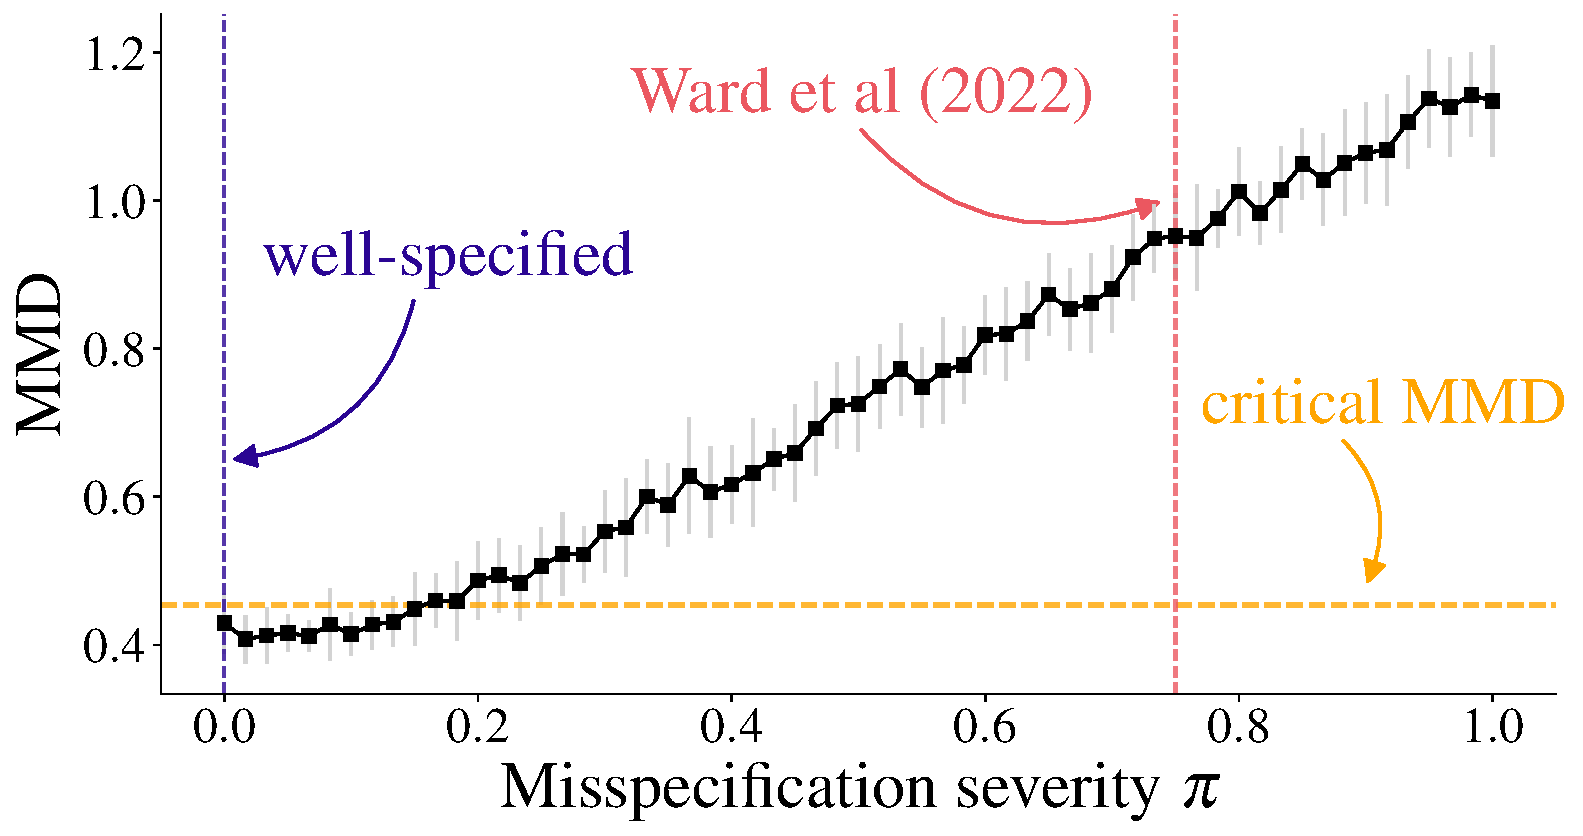
\includegraphics[width=\linewidth]{plots/cs_mms_mmd.pdf}%
            \caption{MMD as a function of misspecification severity.}%
            \label{fig:cs:mms-mmd}%
        \end{subfigure}\\
        \begin{subfigure}[t]{\linewidth}%
                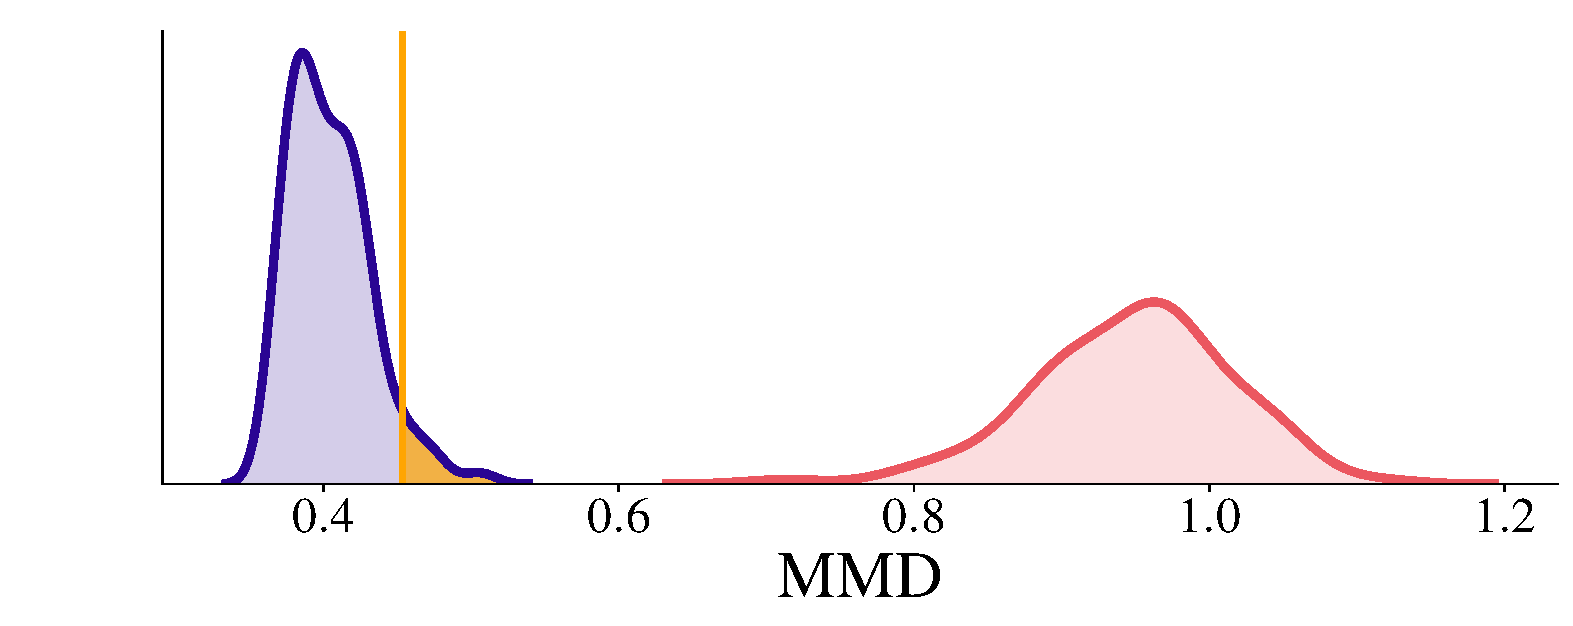
\includegraphics[width=\linewidth]{plots/cs_mms_power.pdf}%
                \caption{Power for $\pi=0.75$.}%
            \label{fig:cs:power}%
        \end{subfigure}%
    \end{minipage}%
    \begin{subfigure}[t]{0.49\linewidth}%
        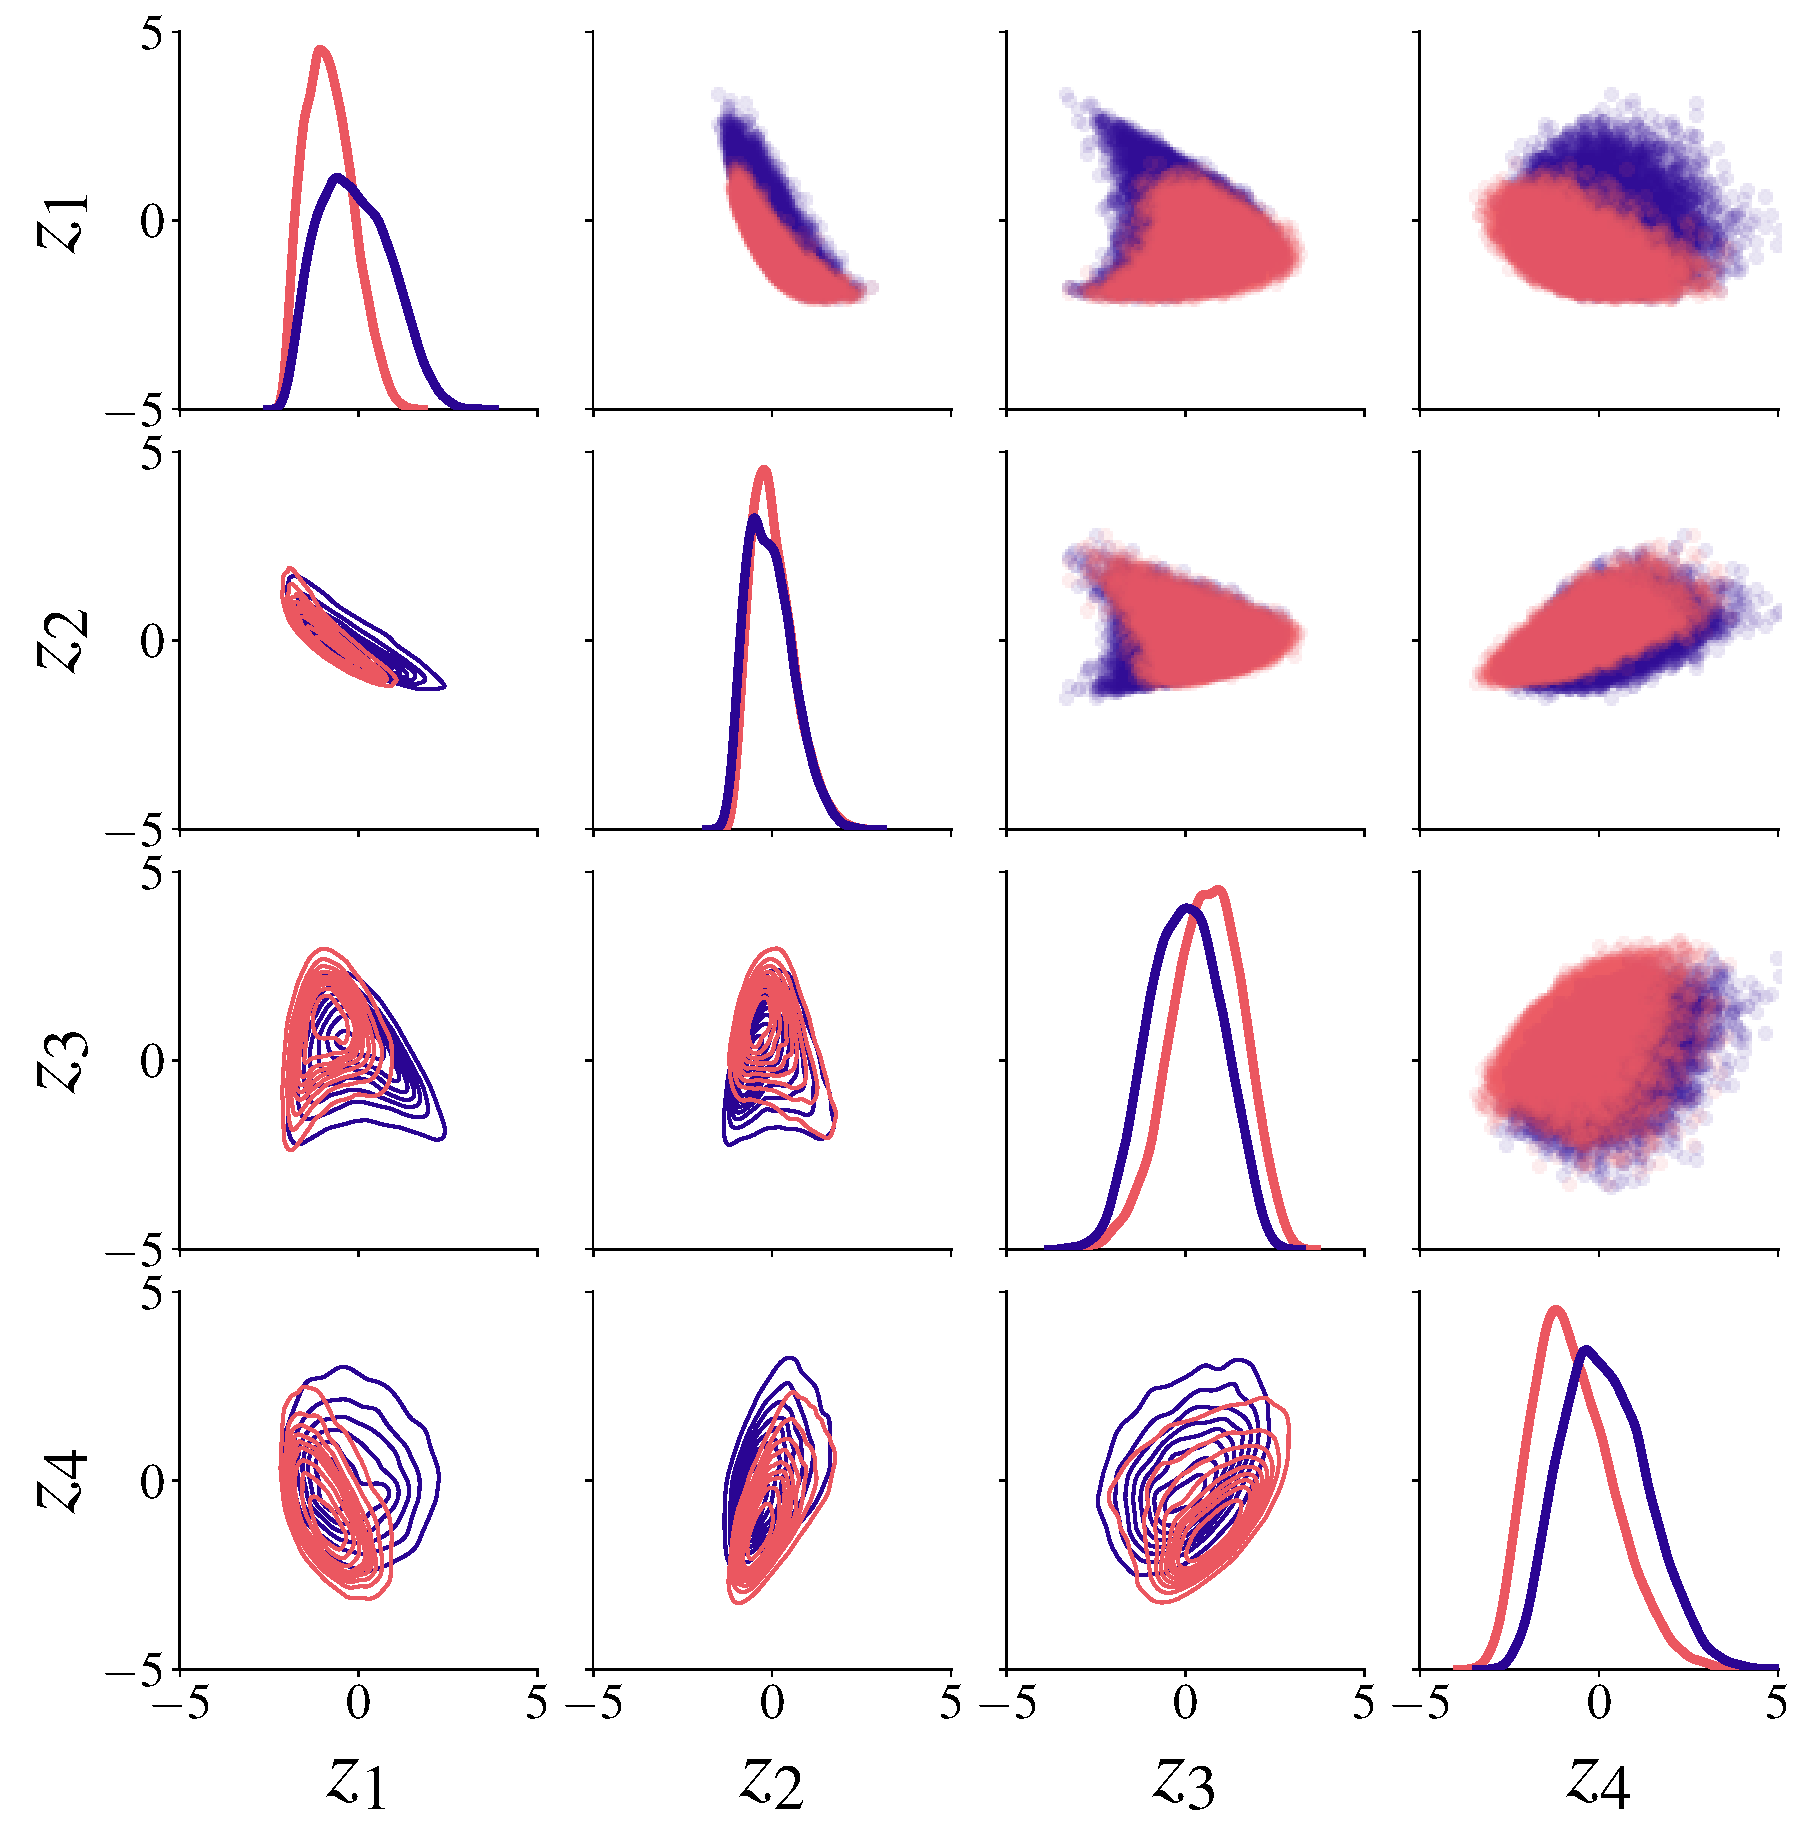
\includegraphics[width=\linewidth]{plots/cs_pairplot.pdf}%
        \caption{Summary space for $\pi=0.75$.}%
        \label{fig:cs-experiment:pairplot}%
    \end{subfigure}\\
    
\includegraphics[width=0.8\linewidth]{plots/cs_legend.pdf}
    \caption{\textbf{Experiment \numberCS.} MMD increases for rising misspecification severity (\subref{fig:cs:mms-mmd}; mean and SD of 20 repetitions). The misspecification studied by \citet{ward_robust_2022} is detectable by our hypothesis test (\subref{fig:cs:power}) and via visual inspection (\subref{fig:cs-experiment:pairplot}).
    The critical MMD value (orange) in (\subref{fig:cs:mms-mmd}) corresponds to the critical MMD in (\subref{fig:cs:power}).
    }
\end{figure}
This experiment illustrates model misspecification detection in a marked point process model of cancer and stromal cells \cite{jones-todd_identifying_2019}.
We use the original implementation of \citet{ward_robust_2022} with hand-crafted summary statistics and showcase the applicability of our method in scenarios where good summary statistics are known.
The inference parameters are three Poisson rates $\lambda_c, \lambda_p, \lambda_d$, and the setup in \citet{ward_robust_2022} extracts four hand-crafted summary statistics from the 2D plane data: (1--2) number of cancer and stromal cells; (3--4) mean and maximum distance from stromal cells to the nearest cancer cell.
All implementation details are described in Section~\ref{app:cs} in the Appendix.

We achieve misspecification during inference by mimicking necrosis, which often occurs in core regions of tumors.
A Bernoulli distribution with parameter $\pi$ controls whether a cell is affected by necrosis or not.
Consequently, $\pi=0$ implies no necrosis (and thus no simulation gap), and $\pi=1$ entails that all cells are affected.
The experiments by \citet{ward_robust_2022} study a single misspecification, namely the case $\pi=0.75$ in our implementation.
In order to employ our proposed method for model misspecification detection, we add a small summary network $h_{\psib}:\mathbb{R}^4\to\mathbb{R}^4$ consisting of three hidden fully connected layers with $64$ units each.
This network $h_{\psib}$ merely transforms the hand-crafted summary statistics into a $4$-D unit Gaussian (cf.\ \autoref{alg:mms}).

\textit{Results.}
Our MMD misspecification score increases with increasingly severe model misspecification (i.e., increasing necrosis rate $\pi$), see \autoref{fig:cs:mms-mmd}.
What is more, for the single misspecification $\pi=0.75$ studied by \citet{ward_robust_2022}, we illustrate (i) the power of our proposed hypothesis test; and (ii) the summary space distribution for misspecified data.
The power ($1-\beta$) essentially equals $1$, as shown in \autoref{fig:cs:power}: The MMD sampling distributions under the training model ($H_0$) and under the observed data generating process ($\M^*$) are completely separated.
In fact, \autoref{fig:cs-experiment:pairplot} unveils that the induced model misspecification is directly visible in the outputs of the summary network $h_{\psib}$.

\subsection{Experiment \numberDDM: Drift Diffusion Model}
\label{sec:ddm-experiment}
\begin{figure}[t]
    \begin{subfigure}[t]{0.33\linewidth}
        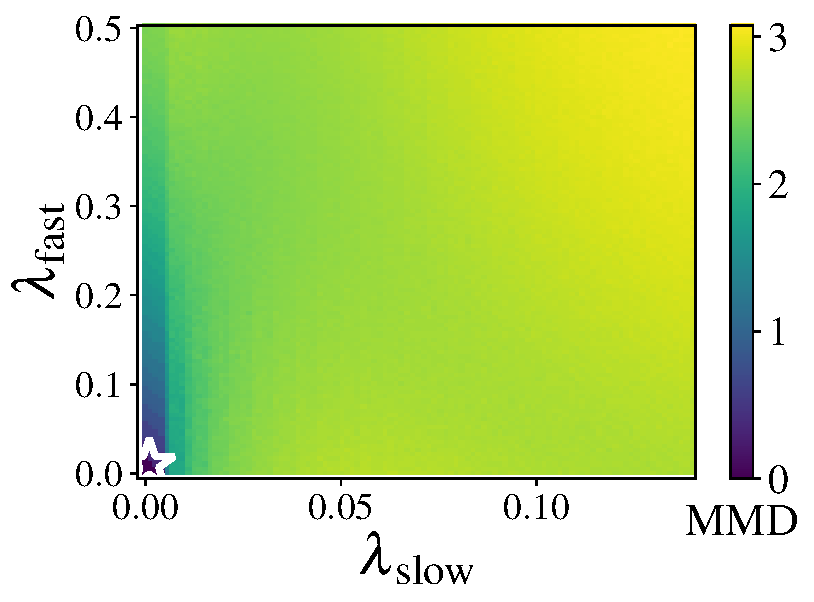
\includegraphics[width=\linewidth]{abf_ddm_unbounded_grid.pdf}
        \caption{MMD as a function of misspecification severity.}
        \label{fig:exp:ddm-mmd-contamination}
    \end{subfigure}
    \hfill
    \begin{subfigure}[t]{0.62\linewidth}
        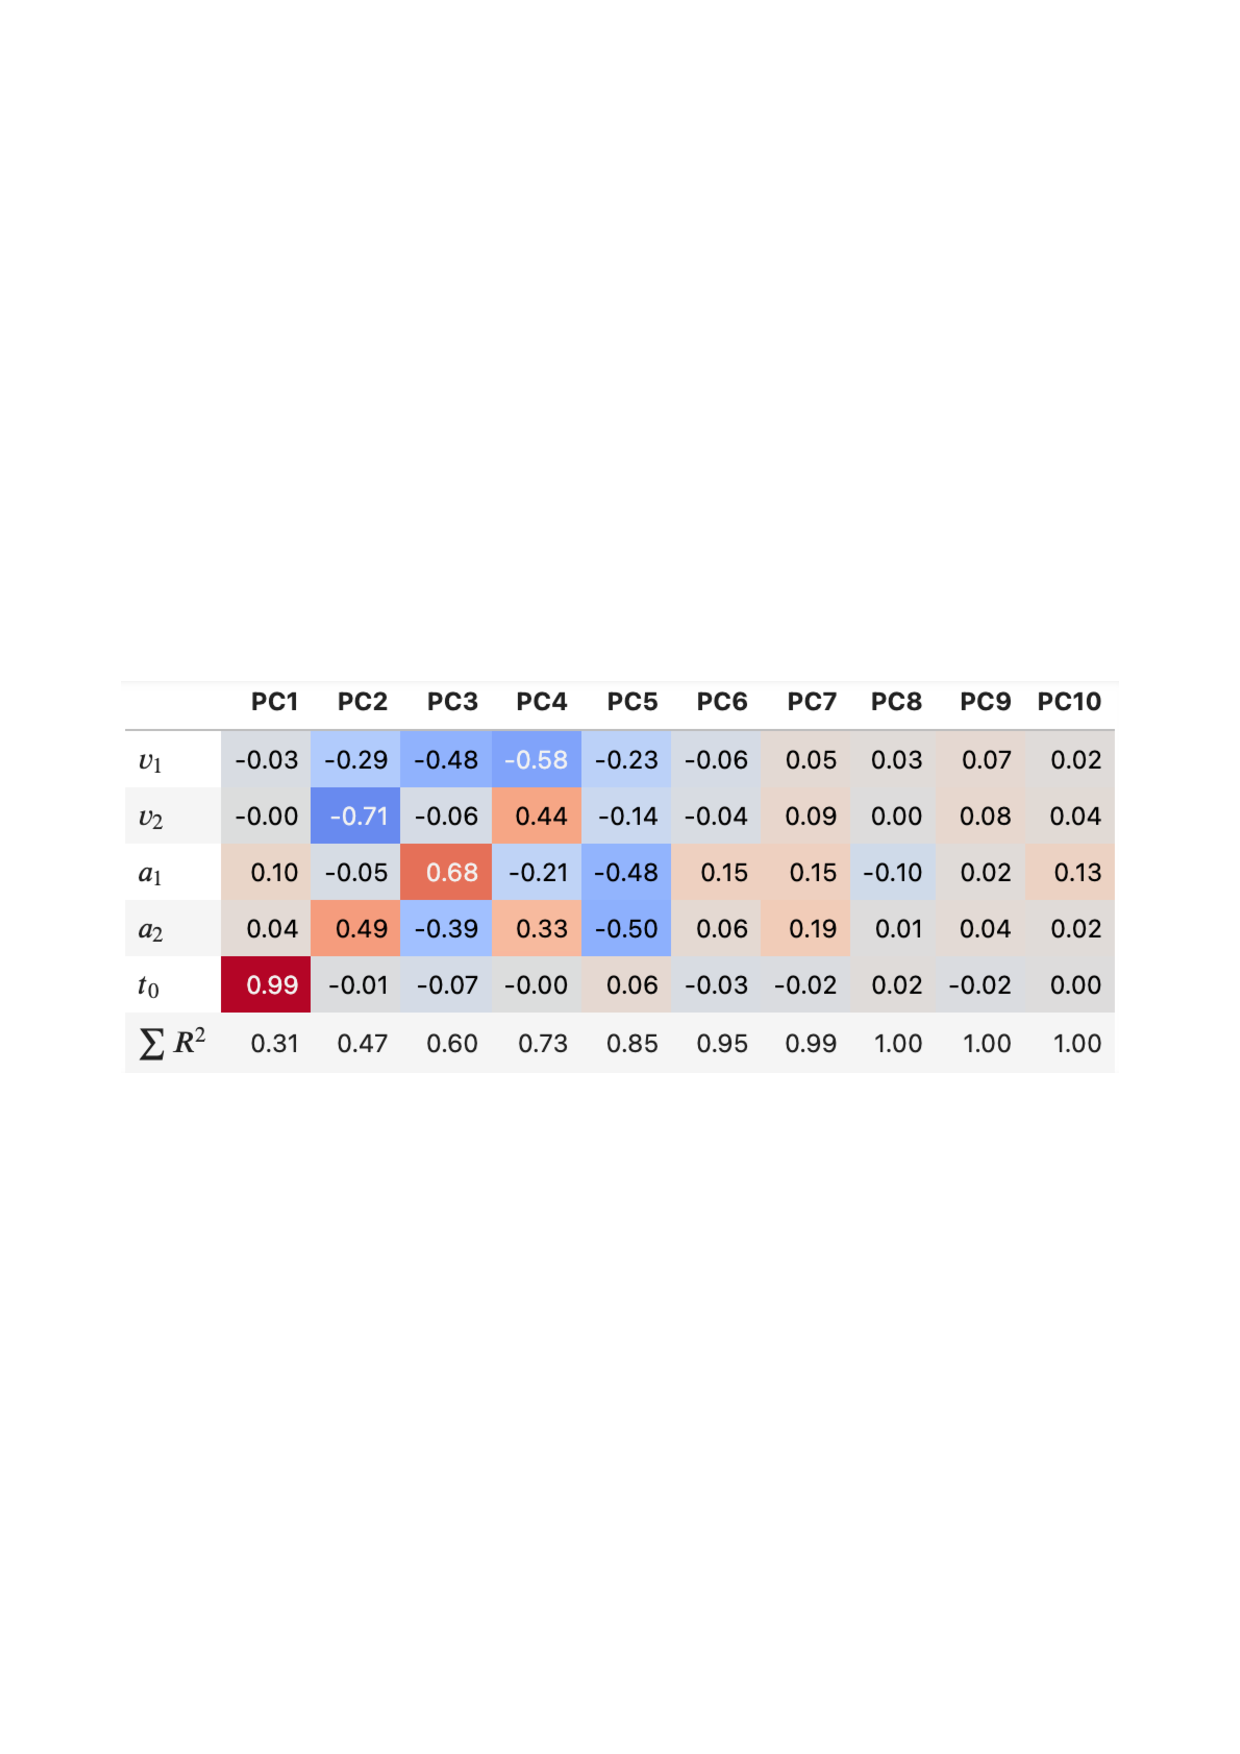
\includegraphics[width=\linewidth]{abf_ddm_unbounded_pca_table.pdf}
        \caption{Correlation between parameters $\thetab$ and principal components (PCs) of learned summary statistics.}
        \label{fig:exp:ddm-pca}
    \end{subfigure}
    \caption{\textbf{Experiment \numberDDM.} Contamination of reaction times is detectable with our method (\subref{fig:exp:ddm-mmd-contamination}), and the principal components from the learned summary statistics coincide with the true parameters $\thetab$ (\subref{fig:exp:ddm-pca}).
    White star indicates the configuration for the well-specified model (i.e., training model $\M$ without contamination).}
    \label{fig:exp:ddm-figure}
\end{figure}
This experiment aims to (i) apply the new optimization objective to a complex model of decision making; (ii) illustrate the effect of dimensionality reduction (principal component analysis); (iii) tackle strategies to determine the required number of learned summary statistics in more complex applications; and (iv) compare the posterior estimation of BayesFlow under a misspecified model with the estimation provided by the Stan implementation of HMC-MCMC \cite{Carpenter2017, Stan2022} as a current gold-standard for Bayesian inference.

We focus on the drift diffusion model (DDM)---a cognitive model describing reaction times (RTs) in binary decision tasks \cite{Ratcliff2008} which is well amenable to amortized inference \cite{Radev2020bayesflow-cognition}.
The DDM assumes that perceptual information for a choice alternative accumulates continuously according to a Wiener diffusion process. 
Thus, the change in information $\diff x_j$ in experimental condition $j$ follows a random walk with drift and Gaussian noise: $\mathrm{d}x_j = v\mathrm{d}t + \xi \sqrt{\mathrm{d}t}$ with $\xi\sim\mathcal{N}(0, 1)$.
% \begin{equation}
%     \mathrm{d}x_j = v\mathrm{d}t + \xi \sqrt{\mathrm{d}t}
%     \quad\text{with}\quad
%     \xi\sim\mathcal{N}(0, 1).
% \end{equation}
Our model implementation assumes five free parameters $\thetab = (v_1, v_2, a_1, a_2, t_0)$ which produce $2$-dimensional data stemming from two simulated conditions.
The summary network is a permutation-invariant network which reduces $i.\,i.\,d.\ $RT data sets to $S=10$ summary statistics each.
We realize a simulation gap by simulating typically observed contaminants: fast guesses (\eg, due to inattention), very slow responses (\eg, due to mind wandering), or a combination of the two.
The parameter $\lambda$ controls the fraction of the observed data which is contaminated  (see Section~\ref{sec:app:ddm} in the Appendix for implementation details).
For the comparison with Stan, we simulate $100$ uncontaminated DDM data sets and three scenarios (fast guesses, slow responses, fast and slow combined) with a fraction of $\lambda = 10\%$ contaminants.

\textit{Results.} During inference, our criterion reliably detects the induced misspecifications: Increasing fractions $\lambda$ of contaminants (fast, slow, and combined) manifest themselves in increasing MMD values (see \autoref{fig:exp:ddm-mmd-contamination}).
The results of applying PCA to the summary network outputs $\{\observed{\z}^{(n)}\}$ for the well-specified model (no contamination) are illustrated in \autoref{fig:exp:ddm-pca}.
We observe that the first five principal components exhibit a large overlap with the true model parameters $\thetab$ and jointly account for 85\% of the variance in the summary output.
Furthermore, the drift rates and decision thresholds within conditions are entangled (\ie, $v_1, a_1$ and $v_2, a_2$).
This entanglement mimics the strong posterior correlations observed between these two parameters.
In practical applications, dimensionality reduction might act as a guideline for determining the number of minimally sufficient summary statistics or parameter redundancies for a given problem.

\begin{table}[b]
    \centering
    \renewcommand{\arraystretch}{1.2}
    \begin{tabular}{l|c|c}
        \textbf{Model (Contamination)} & \textbf{Posterior error MMD} & \textbf{Summary space MMD}\\
        \hline
        $\M_{\ }$: Uncontaminated                  & $0.25\,[0.13, 0.56]$    & $0.45\,[0.42, 0.52]$ \\
        $\M_{1}$: Fast contaminants               & $2.66\,[1.44, 3.40]$    & $2.68\,[2.61, 2.74]$ \\
        $\M_{2}$: Slow contaminants               & $0.55\,[0.23, 1.01]$    & $1.18\,[1.13, 1.26]$ \\
        $\M_{3}$: Fast \& slow contaminants      & $1.90\,[0.83, 3.18]$    & $2.33\,[2.19, 2.43]$
    \end{tabular}
    \caption{
    \textbf{Experiment \numberDDM.} Posterior error of the approximate neural posterior (MMD to Stan samples; median and 95\% CI).
    The bootstrapped MMD values for the summary statistics of the $100$ investigated data sets and $1\,000$ samples from the uncontaminated model $\M$
    illustrate that posterior errors are mirrored by anomalies in the summary space and thus detectable.
    }
    \label{tab:ddm:stan-bf}
\end{table}

For the comparison with Stan, we juxtapose $4\,000$ samples from the approximate neural posterior with $4\,000$ samples obtained from the Stan sampler after ensuring MCMC convergence and sufficient sampling efficiency for each data set (see \autoref{fig:exp:ddm:stan-bf} for an illustration). 
Because Stan is currently considered state-of-the-art for likelihood-based Bayesian inference, we assume the Stan samples are representative of the \emph{correct posterior under the potentially misspecified model} (see Section~\ref{sec:posterior-inference-errors}).
In order to quantify the difference between the posterior samples from BayesFlow and Stan, we use the MMD criterion as well.
When no model misspecification is present, the posterior samples from BayesFlow and Stan match almost perfectly (see \autoref{fig:exp:ddm:stan-bf:clean}).
This means that our augmented optimization objective still enables correct posterior approximation under well-specified models.
In contrast, the results in \autoref{fig:exp:ddm:stan-bf:slow} and \autoref{tab:ddm:stan-bf} clearly indicate that the amortized posteriors deteriorate as a result of the induced misspecification.
Moreover, these results closely mirror the overall detectability of misspecification obtained by matching the summary representations of $1000$ data sets from the uncontaminated process with the representations of the $100$ data sets for each of the above scenarios via MMD (see \autoref{tab:ddm:stan-bf}).

\subsection{Experiment \numberCovid: Epidemiological Model for COVID-19}\label{sec:experiment-covid}
\begin{figure}[t]
\centering
    \begin{subfigure}[t]{.53\linewidth}
        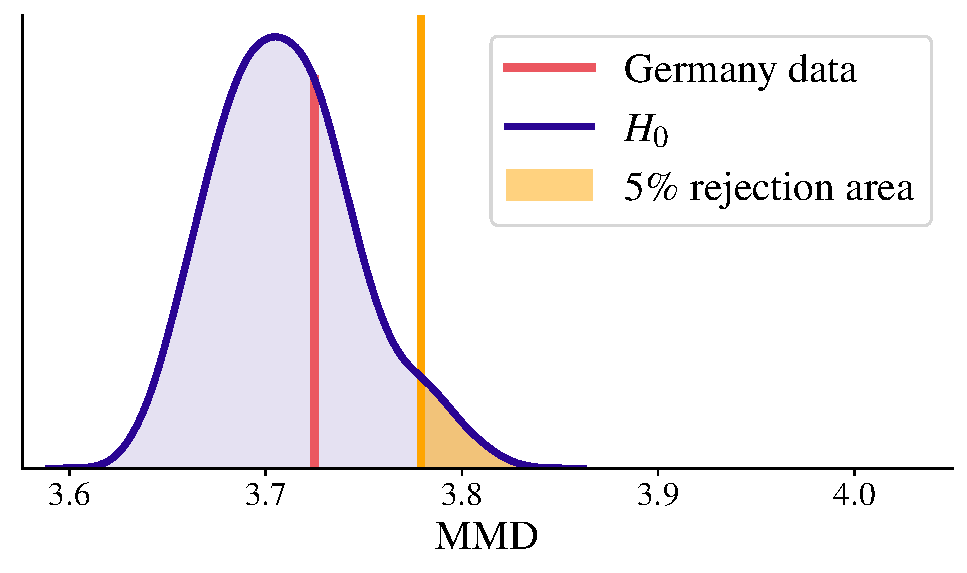
\includegraphics[width=\linewidth]{COVID_real_data_MMD_H0.pdf}
        \caption{Representation of Germany's COVID-19 time series with respect to the MMD distribution under the null hypothesis $H_0: p^*(\x)=p(\x\given\mathcal{M})$.}
        \label{fig:exp:covid:mmd-real-data}
    \end{subfigure}
    \hfill
    \begin{subfigure}[t]{.44\linewidth}
        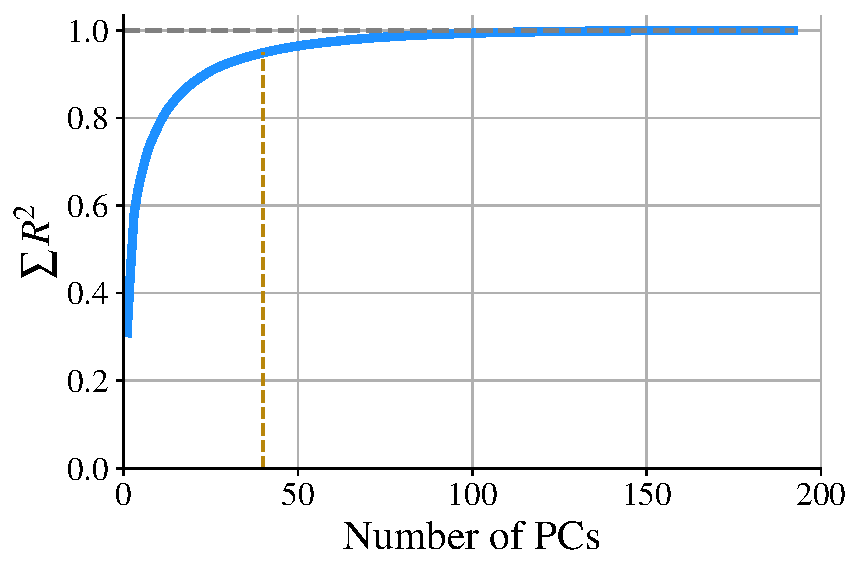
\includegraphics[width=\linewidth]{COVID_PCA_explained_variance.pdf}
        \caption{Cumulative explained variance ratio for the summary network output as a function of the number of principal components (PC).}
        \label{fig:exp:covid:PCA-exp-var}
    \end{subfigure}
    \caption{\textbf{Experiment \numberCovid}. The observed German COVID-19 time series is well-specified with respect to the training model $\M$ (\subref{fig:exp:covid:mmd-real-data}), and the first $40$ principal components jointly account for $95\%$ of the variance in the summary network outputs (\subref{fig:exp:covid:PCA-exp-var}; golden dashed line).}
    \label{fig:exp:COVID:real-data-and-PCA}
\end{figure}
\begin{comment}
\textit{Aims.} The third experiment applies our new optimization objective to a dynamic model of the early COVID-19 outbreak in Germany \cite{outbreak}. It aims to i) fully replicate the results obtained in \cite{outbreak} using a large structured summary space of size $S = 192$; ii) demonstrate the utility of MMD to detect simulation gaps in the context of non-trivial complex models; iii) investigate the statistical power and characteristics of the sampling-based MMD hypothesis test in a realistic modeling scenario; and iv) showcase the use of MMD as a proxy for increasing model trustworthiness in socially relevant applications.
\end{comment}

Compartmental models in epidemiology are very popular for inferring relevant disease parameters, simulating possible outbreak scenarios, and projecting future outcomes \cite{covid_germany}.
Given the abundance of such models and their increasing complexity, the importance of detecting simulation gaps for trustworthy inference is two-fold. 
First, since substantial conclusions are based on the posterior distributions of model parameters, it is important that these distributions are formally correct even when models do not capture all relevant real-world factors. 
Second, given the dynamic aspect of these models, it is important to detect if an initially well-specified model becomes misspecified at a later time, so the model and its predictions can be amended.

As a final real-world example, we thus focus on a high-dimensional compartmental model representing the early months of the COVID-19 pandemic in Germany \cite{outbreak}.
Here, we investigate the utility of our distribution matching method to detect simulation gaps in a much more realistic and non-trivial extension of the SIR settings in \citet{lueckmann_benchmarking_2021} and  \citet{ward_robust_2022} with substantially increased complexity.\footnote{The SIR experiment from \citet{ward_robust_2022} induces misspecification through delayed reporting. 
This is modeled via $\M_2$ in our experiment.
The additional models $\M_1, \M_3$ in our experiment are extensions to the existing literature on model misspecification.}
Moreover, we perform inference on real COVID-19 data from Germany and use our new method to test whether the model used in \citet{outbreak} is misspecified, possibly undermining the trustworthiness of political conclusions that are based on the inferred posteriors.
To achieve this, we train a BayesFlow setup identical to \citet{outbreak} but using our new optimization objective (Eq.~\ref{eq:bf_kl_mmd}) to encourage a structured summary space.
We then simulate $1000$ time series from the training model $\mathcal{M}$ and $1000$ time series from three misspecified models: (i) a model $\mathcal{M}_1$ without an intervention sub-model; (ii) a model $\mathcal{M}_2$ without an observation sub-model; (iii) a model $\mathcal{M}_3$ without a latent ``carrier'' compartment \cite{covid_germany}.
%Whereas the first two models are lacking essential components for representing the observed disease dynamics, \citet{covid_germany} have demonstrated good results with a simpler model without a latent ``carrier'' compartment.
%Thus, we expect that simulation gaps will be harder to detect when comparing the outputs of the original model $\mathcal{M}^*$ and model $\mathcal{M}_3$ in summary space.
\begin{table*}[b]
    \centering
    \renewcommand{\arraystretch}{1.2}
    \begin{tabular}{c|ccc|ccc}
        \multirow{2}{*}{\bfseries Model}& 
        \multicolumn{3}{c|}{\bfseries Bootstrap MMD} & 
        \multicolumn{3}{c}{ \bfseries Power ($1-\beta$)} \\
        & $N=1$  & $N=2$ & $N=5$ & $N=1$ & $N=2$ & $N=5$\\
        \hline
        $\mathcal{M}_{\ }$ & $3.70\,[3.65, 3.79]$ & $2.61\,[2.54, 2.91]$ & $1.66\,[1.59, 1.84]$ & --- & --- & ---\\
        $\mathcal{M}_1$ & $3.76\,[3.72, 3.80]$ & $2.86\,[2.62, 3.16]$ & $2.11\,[1.82, 2.50]$ & $.998$ & $.958$ & $\approx1.0$ \\
        $\mathcal{M}_2$ & $3.80\,[3.73, 3.83]$ & $2.81\,[2.65, 3.00]$ & $2.01\,[1.82, 2.19]$ & $.789$ & $.804$ & $\approx1.0$ \\
        $\mathcal{M}_3$ & $3.78\,[3.74, 3.83]$ & $2.81\,[2.68, 3.11]$ & $2.07\,[1.92, 2.41]$ & $.631$ & $.690$ & $\approx1.0$ \\
    \end{tabular}
    \caption{
    \textbf{Experiment \numberCovid.} Results for different variations of the COVID-19 compartmental model.
    We report the median and 95\% CI of 100 bootstrap samples. 
    }
    \label{tab:covid19-models-mmd}
\end{table*}
\textit{Results.}
\autoref{tab:covid19-models-mmd} shows the MMD between the summary representation of $N=1,2,5$ bootstrapped time series from each model and the summary representation of the $1000$ time series from model $\mathcal{M}$ (see Section~\ref{sec:app:bootstrap} for bootstrapping details).
We also calculate the power ($1-\beta$) of our hypothesis test for each misspecified model under the sampling distribution estimated from $1\,000$ samples of the $1\,000$ time series from $\mathcal{M}$ at a type I error probability of $\alpha=.05$.
We observe that the power of the test rapidly increases with more data sets and the Type II error probability ($\beta$) is essentially zero for as few as $N=5$ time series (see \autoref{fig:app:covid:power}).

As a next step, we pass the reported COVID-19 data between 1 March and 21 April 2020 \citep[data from][under CC BY 4.0 license]{dong_interactive_2020} through the summary network and compute the critical MMD value for a sampling-based hypothesis test with an $\alpha$ level of $.05$ (see \autoref{fig:exp:covid:mmd-real-data}). 
The MMD of the Germany data is well below the critical MMD value (it essentially lies in the bulk of the distribution), leading to the conclusion that the assumed training model $\M$ is well-specified for this time period.
Finally, we perform linear dimensionality reduction (PCA) on the summary space and find that the first 40 principal components jointly explain $95\%$ of the variance in the $192$-dimensional summary space outputs (see \autoref{fig:exp:covid:PCA-exp-var}). 
Thus, a $40$-dimensional learned summary vector might provide a good approximation of the true (unknown) minimally sufficient summary statistics and render inference less fragile in the face of potential misspecifications (cf.\ \textbf{Experiment \numberGaussianMeans}).

\begin{figure}[t]
    \centering
    \begin{tabular}{cccc}
    & {\Large$N=1$} & {\Large$N=2$} & {\Large$N=5$}\\
    \rotatebox[origin=c]{90}{\raisebox{0.1cm}{\colsquare{observedcolor}}\Large$\M_1$} & 
    \raisebox{-0.48\height}{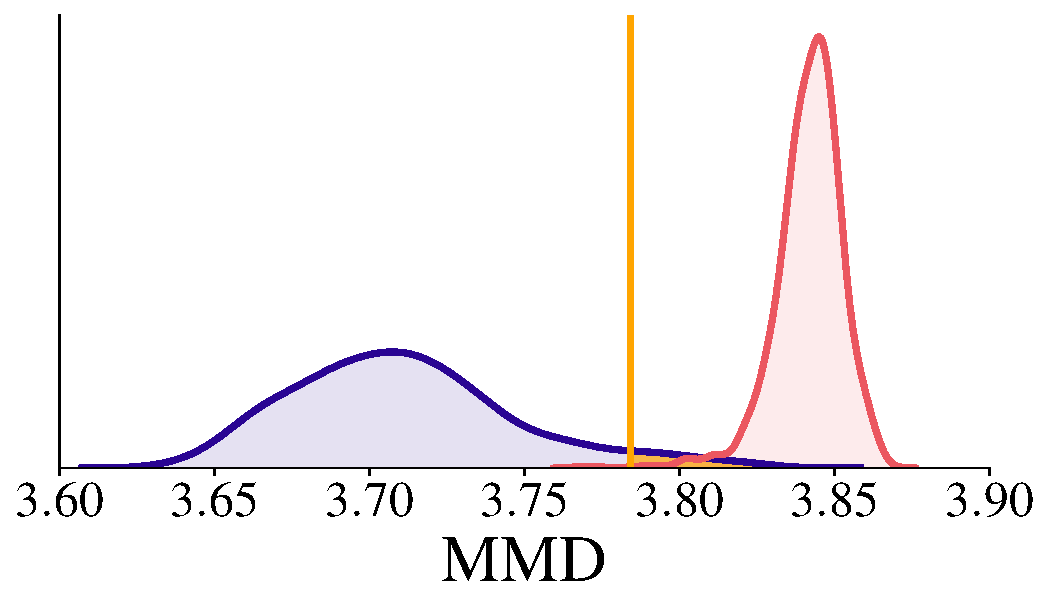
\includegraphics[width=.28\linewidth]{COVID_power_N1_M1.pdf}} &
    \raisebox{-0.48\height}{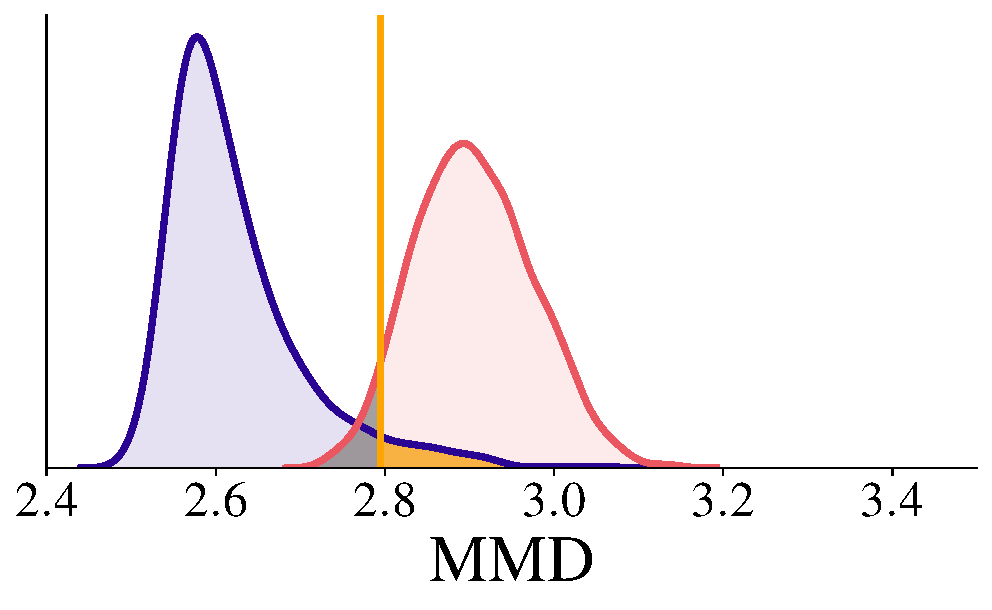
\includegraphics[width=.28\linewidth]{COVID_power_N2_M1.pdf}} &
    \raisebox{-0.48\height}{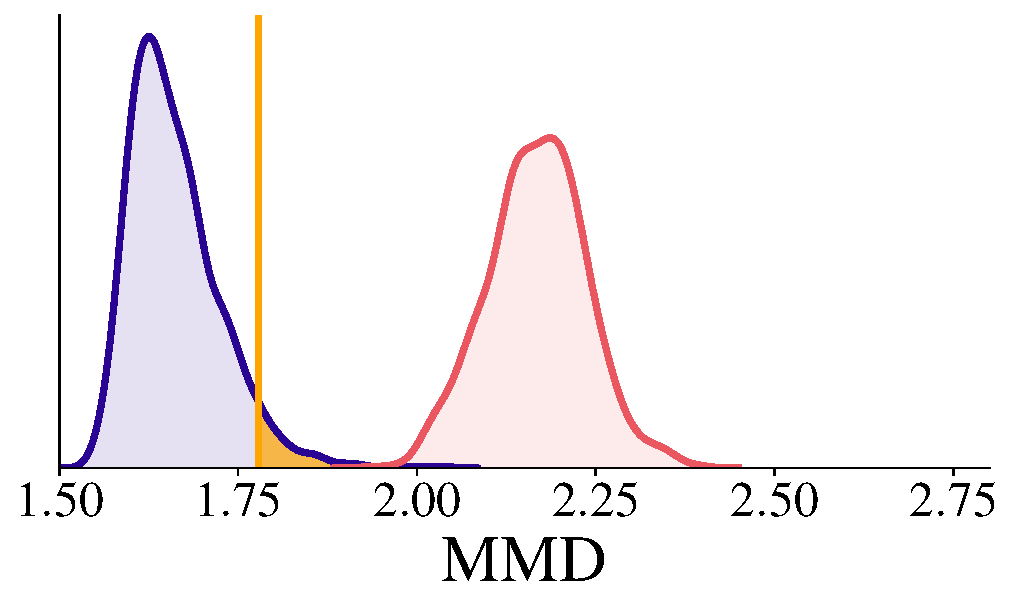
\includegraphics[width=.28\linewidth]{COVID_power_N5_M1.pdf}}\\
    \rotatebox[origin=c]{90}{\raisebox{0.1cm}{\colsquare{observedcolor}}\Large$\M_2$} & 
    \raisebox{-0.48\height}{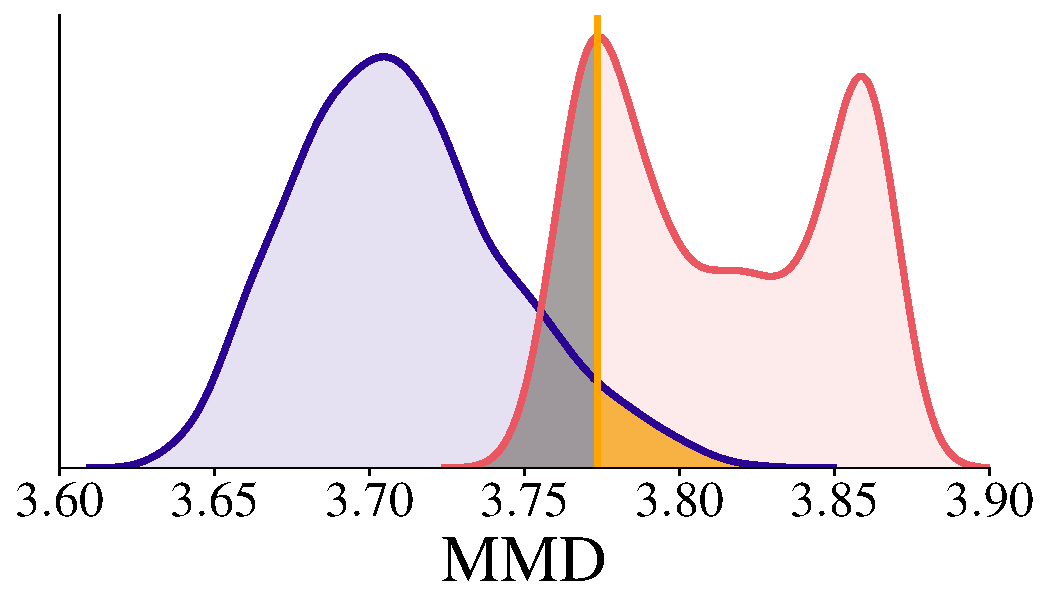
\includegraphics[width=.28\linewidth]{COVID_power_N1_M2.pdf}} &
    \raisebox{-0.48\height}{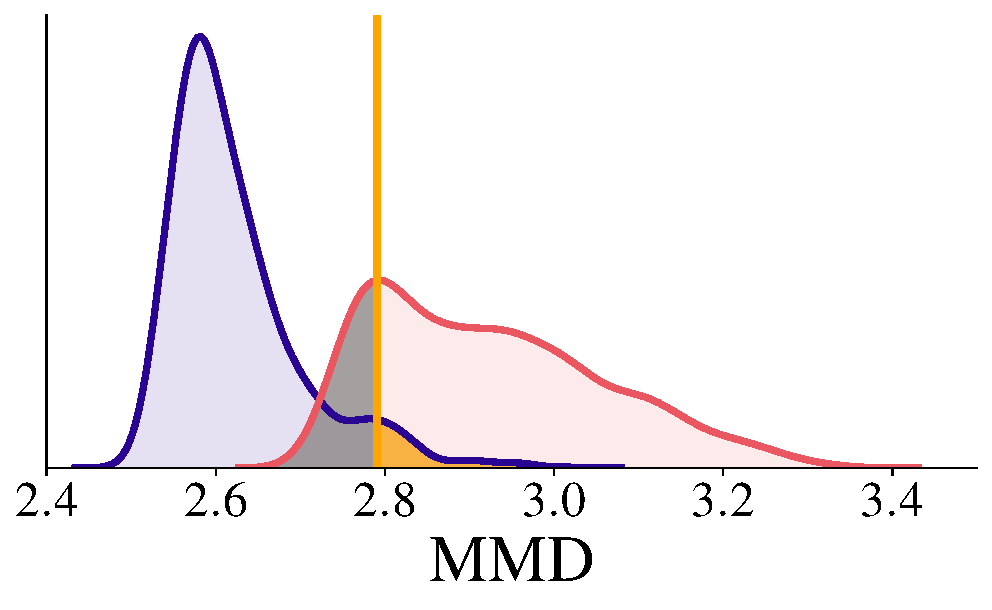
\includegraphics[width=.28\linewidth]{COVID_power_N2_M2.pdf}} &
    \raisebox{-0.48\height}{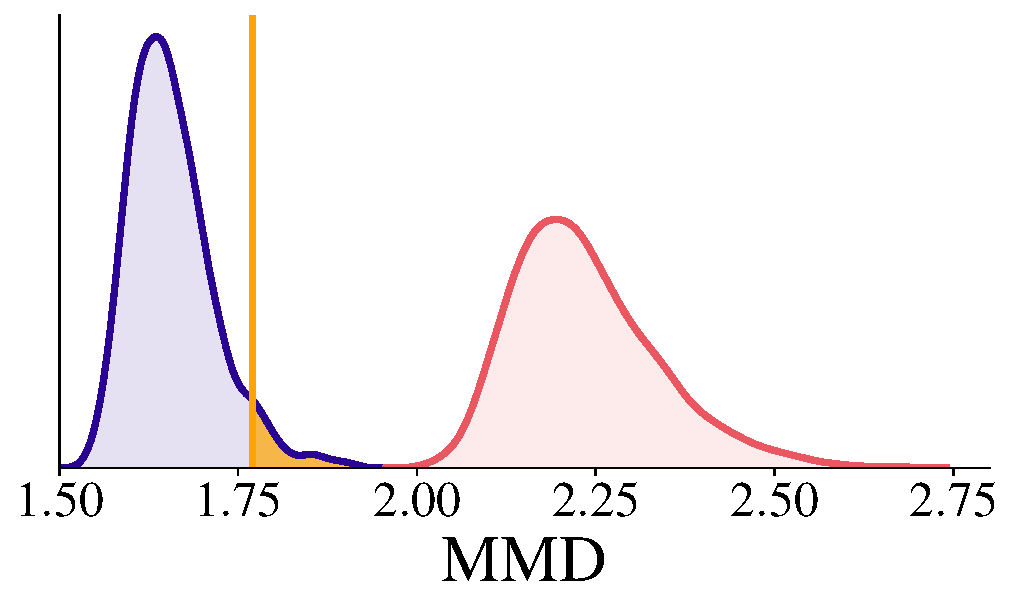
\includegraphics[width=.28\linewidth]{COVID_power_N5_M2.pdf}}\\
    \rotatebox[origin=c]{90}{\raisebox{0.1cm}{\colsquare{observedcolor}}\Large$\M_3$} & 
    \raisebox{-0.48\height}{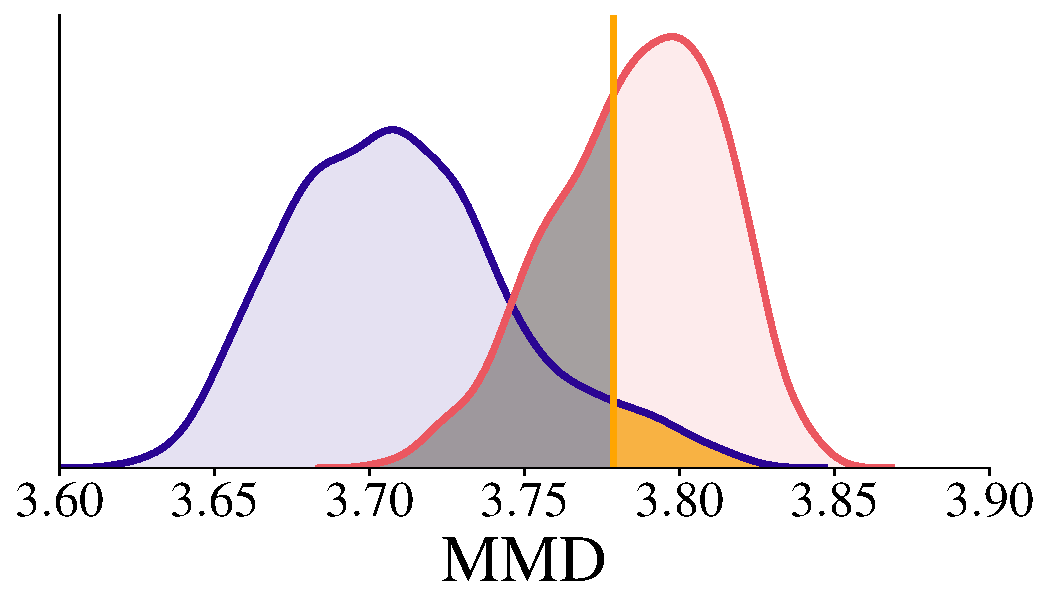
\includegraphics[width=.28\linewidth]{COVID_power_N1_M3.pdf}} &
    \raisebox{-0.48\height}{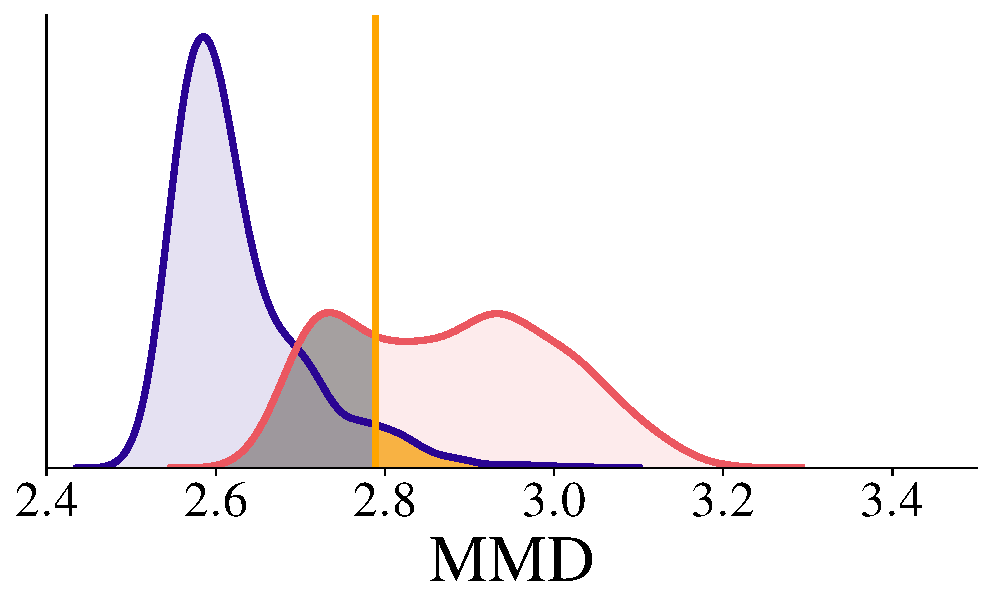
\includegraphics[width=.28\linewidth]{COVID_power_N2_M3.pdf}} &
    \raisebox{-0.48\height}{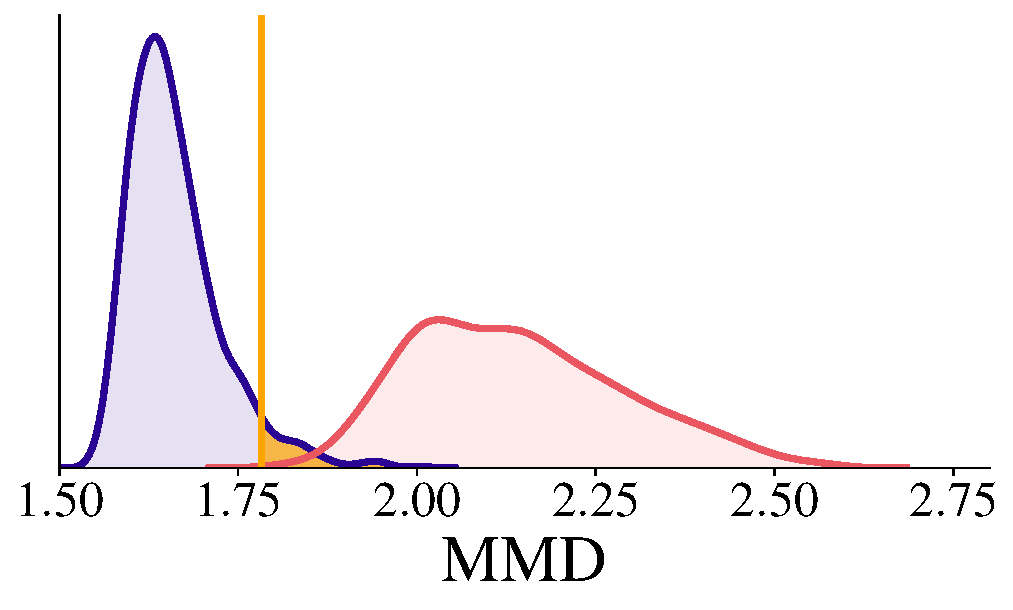
\includegraphics[width=.28\linewidth]{COVID_power_N5_M3.pdf}}\\
    \end{tabular}\\
    \includegraphics[width=1.0\linewidth]{COVID_power_legend.pdf}
    \caption{\textbf{Experiment \numberCovid.} Detailed illustration of the power analysis. \autoref{tab:covid19-models-mmd} contains the test power ($1-\beta$) for each scenario, and as few as $N=5$ observed data sets suffice to achieve a negligible type II error $\beta\approx 0$.}
    \label{fig:app:covid:power}
\end{figure}

% \begin{figure}[h]
%     \centering
%     \begin{subfigure}[t]{.32\linewidth}
%         \includegraphics[width=\linewidth]{COVID_power_N1_M1.pdf}
%         \caption{\colsquare{observedcolor}$\mathcal{M}_1, N=1, 1-\beta=.998$}
%     \end{subfigure}
%     \hfill
%     \begin{subfigure}[t]{.32\linewidth}
%         \includegraphics[width=\linewidth]{COVID_power_N2_M1.pdf}
%         \caption{\colsquare{observedcolor}$\mathcal{M}_1, N=2, 1-\beta=.958$}
%     \end{subfigure}
%     \hfill
%     \begin{subfigure}[t]{.32\linewidth}
%         \includegraphics[width=\linewidth]{COVID_power_N5_M1.pdf}
%         \caption{\colsquare{observedcolor}$\mathcal{M}_1, N=5, 1-\beta\approx 1.0$}
%     \end{subfigure}\\
%     \vspace*{0.5cm}
%     \begin{subfigure}[t]{.32\linewidth}
%         \includegraphics[width=\linewidth]{COVID_power_N1_M2.pdf}
%         \caption{\colsquare{observedcolor}$\mathcal{M}_2, N=1, 1-\beta=.789$}
%     \end{subfigure}
%     \hfill
%     \begin{subfigure}[t]{.32\linewidth}
%         \includegraphics[width=\linewidth]{COVID_power_N2_M2.pdf}
%         \caption{\colsquare{observedcolor}$\mathcal{M}_2, N=2, 1-\beta=.804$}
%     \end{subfigure}
%     \hfill
%     \begin{subfigure}[t]{.32\linewidth}
%         \includegraphics[width=\linewidth]{COVID_power_N5_M2.pdf}
%         \caption{\colsquare{observedcolor}$\mathcal{M}_2, N=5, 1-\beta\approx 1.0$}
%     \end{subfigure}\\
%     \vspace*{0.5cm}
%     \begin{subfigure}[t]{.32\linewidth}
%         \includegraphics[width=\linewidth]{COVID_power_N1_M3.pdf}
%         \caption{\colsquare{observedcolor}$\mathcal{M}_3, N=1, 1-\beta=.631$}
%     \end{subfigure}
%     \hfill
%     \begin{subfigure}[t]{.32\linewidth}
%         \includegraphics[width=\linewidth]{COVID_power_N2_M3.pdf}
%         \caption{\colsquare{observedcolor}$\mathcal{M}_3, N=2, 1-\beta=.690$}
%     \end{subfigure}
%     \hfill
%     \begin{subfigure}[t]{.32\linewidth}
%         \includegraphics[width=\linewidth]{COVID_power_N5_M3.pdf}
%         \caption{\colsquare{observedcolor}$\mathcal{M}_3, N=5, 1-\beta\approx 1.0$}
%     \end{subfigure}\\
%     \includegraphics[width=1.0\linewidth]{COVID_power_legend.pdf}
%     \caption{\textbf{Experiment \numberCovid.} Detailed illustration of the power analysis.}
%     \label{fig:app:covid:power}
% \end{figure}

\section{Conclusions}\label{sec:discussion}

With this work, we approached a fundamental problem in amortized simulation-based Bayesian inference, namely, capturing posterior errors due to model misspecification.
We argued that misspecified models might cause so-called \emph{simulation gaps}, resulting in deviations between simulations during training time and actual observed data at test time.
We further showed that simulation gaps can be detrimental for the performance and faithfulness of simulation-based inference relying on neural networks.
We proposed to increase the networks' awareness of posterior errors by compressing simulations into a structured latent summary space induced by a modified optimization objective in an unsupervised fashion. 
We then applied the maximum mean discrepancy (MMD) estimator, equipped with a sampling-based hypothesis test, as a criterion to spotlight discrepancies between model-implied and actually observed distributions in summary space.
While we focused on the application to SNPE-C and BayesFlow, the proposed method can be easily integrated into other frameworks with learned or hand-crafted summary statistics as well.

The proposed method can be extended and modified in multiple ways.
While we optimized the summary space to follow a spherical Gaussian distribution, our method is likewise applicable to other latent distributions.
For example, a heavy-tailed summary distribution (\eg, $\alpha$-stable distributions with tunable tail parameters) would reduce the impact of outliers in latent space.
%Initial experiments indicate that such variations can lower posterior errors while still maintaining the ability to detect simulation gaps. %(cf. \autoref{fig:exp:mvn-means:MMD-error}).
Furthermore, the sampling-based hypothesis test in summary space can be readily replaced with a more sophisticated statistical testing regime for out-of-distribution detection \cite{bergamin_model-agnostic_2022}.
The idea of \citet{frazier_model_2020} to detect simulation gaps by posterior discrepancies in an ensemble of differently configured approximator instances is interesting, and future work might incorporate this into simulation-based neural inference.
In addition, considerations on information geometry and non-Euclidean spaces might guide future research into building more flexible latent spaces and distance metrics \cite{info_geo}.
Our software implementations are openly available at \href{https://www.github.com/marvinschmitt/ModelMisspecificationBF}{\textrm{github.com/marvinschmitt/ModelMisspecificationBF}} and can be seamlessly integrated into an end-to-end workflow for amortized simulation-based inference.

\begin{comment}
Our experiments confirm the utility of the new optimization and detection methods.  
Furthermore, we observed an interesting connection between detectability, posterior errors, and latent space dimensionality.
The results of \textbf{Experiment \numberGaussianMeans} suggest a trade-off between model misspecification detection and posterior inference error for different numbers of learnable summary statistics (see \autoref{fig:exp:mvn-means:MMD-error:likelihood-noise}).
A minimally sufficient summary network failed to detect carefully designed noise and simulator misspecifications, whereas an overcomplete summary network was able to capture these differences. 
However, using the overcomplete summary network resulted in remarkably worse inference (as measured by deviations from the analytic posterior) under model misspecification. 

This finding raises the question of how to determine the number of optimal learnable summary statistics in practical applications. 
While an intuitive heuristic might suggest ``the more, the merrier'', our analyses in \textbf{Experiment \numberGaussianMeans} beg to differ depending on the modeling goals.
If the focus in a critical application lies in detecting potential simulation gaps, it would be advantageous to utilize a large (overcomplete) summary vector.
However, modelers might also desire a network which is as robust as possible during inference.
In this case, they might opt for a dimensionality reduction approach:
In \textbf{Experiment \numberDDM} and \textbf{Experiment \numberCovid}, we illustrate how PCA can be utilized to estimate the number of minimally sufficient summary statistics for an opaque model.
Accordingly, using a vector of minimally sufficient statistics might render inference networks more robust against simulation gaps, but also hide potential errors. 

To sum up, the current work presents an endeavor towards a systematic workflow to detect model misspecification and posterior inference errors in simulation-based inference with invertible neural networks.
We delineated different forms of model misspecification and investigated new methods for reliable detection of simulation gaps and inference errors.
The proposed methods are openly available\footnote{The development version of the overarching BayesFlow project is available in the public repository at \url{https://github.com/stefanradev93/BayesFlow}. Integration to PyPI is planned.} and can be seamlessly integrated into the workflow for end-to-end simulation-based Bayesian parameter estimation with invertible neural networks.
\end{comment}




% Acknowledgements should go at the end, before appendices and references

\acks{This research was supported by the Cyber Valley Research Fund (grant number: CyVy-RF-2021-16), the Deutsche Forschungsgemeinschaft (DFG, German Research Foundation) under Germany’s Excellence Strategy -- EXC-2075 - 390740016 (the Stuttgart Cluster of Excellence SimTech) and EXC-2181 - 390900948 (the Heidelberg Cluster of Excellence STRUCTURES), the Deutsche Forschungsgemeinschaft (DFG, German Research Foundation; grant number GRK 2277 ``Statistical Modeling in Psychology''), and the Informatics for Life initiative funded by the Klaus Tschira Foundation.
The authors gratefully acknowledge the support and funding.
}

% Manual newpage inserted to improve layout of sample file - not
% needed in general before appendices/bibliography.


\appendix
\clearpage
\begin{center}
    \Large\bfseries Appendix
\end{center}

\counterwithin{figure}{section}

\section{Implementation Details}


\subsection{5D Gaussian with Covariance (Experiment \numberGaussianMeansCov)}
\label{sec:app:mvn-full}
The normal-inverse-Wishart prior $\NIW(\mub, \Sigmab\given\mub_0, \lambda_0, \Psib_0, \nu_0)$ implies a hierarchical prior. 
Suppose the covariance matrix $\Sigmab$ has an inverse Wishart distribution $\mathcal{W}^{-1}(\Sigmab\given\Psib_0, \nu_0)$  and the mean vector $\mub$ has a multivariate normal distribution $\mathcal{N}(\mub\given\mub_0, \frac{1}{\lambda_0}\Sigmab)$, then the tuple $(\mub, \Sigmab)$ has a normal-inverse-Wishart distribution $\NIW(\mub, \Sigmab\given\mub_0, \lambda_0, \Psib_0, \nu_0)$.
Finally, the likelihood is Gaussian:$\x_k\sim\mathcal{N}(\mub, \Sigmab)\;\text{for}\; k=1,\ldots, K$.

For a multivariate Gaussian with unknown mean and unknown covariance matrix, the analytic joint posterior $p(\mub_p, \Sigmab_p\given\x)$ follows a normal-inverse Wishart distribution again:
\begin{equation}
\begin{aligned}
    (\mub_p, \Sigmab_p \given \x) & \sim\text{N-}\mathcal{W}^{-1}(\mub_p, \Sigmab_p\given\mub_K, \lambda_K, \Psib_K, \nu_K)\quad\text{with}\\
    \mub_K & = \dfrac{\lambda_0\mub_0 + K\bar{\x}}{\lambda_0+K},\quad 
    \lambda_K =\lambda_0+K,\quad
    \nu_K  = \nu_0+K,\\
    \Psib_K & = \Psib_0+\sum\limits_{k=1}^K(\x_k-\bar{\x})(\x_k-\bar{\x})^T+\dfrac{\lambda_0 K}{\lambda_0 + K}(\bar{\x}-\mub_0)(\bar{\x}-\mub_0)^T
\end{aligned}
\end{equation}
The marginal posteriors for $\mub_p$ and $\Sigmab_p$ then follow as \cite{Murphy2007}:
\begin{equation}\label{eq:mvn-full-cov:analytic-posterior:marginal}
\begin{aligned}
    \mub_p & \sim t_{\nu_K-D-1}\Big(\mub_p\,\Big|\,\mub_K, \frac{\Psib_K^{-1}}{\lambda_K(\nu_K-D+1)}\Big)\\
    \Sigmab_p & \sim \mathcal{W}^{-1}(\Sigmab_p\given\Psib_K, \nu_K)
\end{aligned}
\end{equation}

The model $\mathcal{M}$ used for training the networks as well as the types of induced model misspecifications are outlined in \autoref{tab:app:mvn-full-MMS}.
\begin{table*}[b]
    \centering
    \scriptsize
    \begin{tabular}{l|ll}
        \bfseries Model &\bfseries Prior &\bfseries Likelihood\\
        \hline
        $\mathcal{M}$ (No MMS) &
        $\big(\mub, \Sigmab\big)\sim\NIW(\mub_0=\0, \lambda_0=5, \Psib=\mathbb{I},\nu=10)$ &
        $\x_k\sim\mathcal{N}(\mub, \Sigmab)$
        \\
        $\mathcal{M}_P$ (Prior) &
        $\big(\mub, \Sigmab\big)\sim\NIW(\mub_0\neq\0, \lambda_0=5, \Psib=\tau_0\mathbb{I},\nu=10)$&
        $\x_k\sim\mathcal{N}(\mub, \Sigmab)$\\
        $\mathcal{M}_S$ (Simulator) &
        $\big(\mub, \Sigmab\big)\sim\NIW(\mub_0=\0, \lambda_0=5, \Psib=\mathbb{I},\nu=10)$&
        $\x_k\sim t_{\text{df}}(\mub, \Sigmab),\quad\text{df}\in\mathbb{N}_{>0}$
        \\
        $\mathcal{M}_N$ (Noise)&
        $\big(\mub, \Sigmab\big)\sim\NIW(\mub_0=\0, \lambda_0=5, \Psib=\mathbb{I},\nu=10)$& 
        $\x_k\sim\lambda\cdot\mathrm{Beta}(2, 5)+(1-\lambda)\cdot\mathcal{N}(\mub, \Sigmab)%, \lambda$%\in[0, 1]
        $
    \end{tabular}
        \caption{Investigated model misspecifications (MMS) for the $5$-dimensional Gaussian with fully estimated covariance matrix. 
    }
    \label{tab:app:mvn-full-MMS}
\end{table*}
In the evaluation, we compare the means of the approximate posterior samples with the first moment of the respective marginal analytic posterior from Eq.~\ref{eq:mvn-full-cov:analytic-posterior:marginal}. 
We evaluate correlation matrices with standard deviations on the diagonal. 
For the $t$ distributed posterior mean and inverse-Wishart distributed posterior covariance, we obtain \cite{Mardia1979}:
\begin{equation}
        \mathbb{E}(\mub_p) =\mub_K,\quad
        \mathbb{E}(\Sigmab_p) =\frac{\Psib_K}{\nu_K-D-1}
\end{equation}

\subsection{Cancer and Stromal Cells (Experiment \numberCS)}\label{app:cs}

As implemented by \citet{ward_robust_2022}, the CS model simulates the development of cancer and stromal cells.
The respective cell counts (total $N_c$, unobserved parents $N_p$, daughters for each parent $N_d^{(i)}$) are stochastically defined through Poisson distributions
\begin{equation}
        N_c \sim \mathrm{Poisson}(\lambda_c),\quad N_p \sim \mathrm{Poisson}(\lambda_c),\quad N_d^{(i)} \sim \mathrm{Poisson}(\lambda_c),\quad i=1,\ldots, N_p.
\end{equation}

The distance based metrics for the hand-crafted summary statistics 3--4 are empirically approximated from 50 stromal cells to avoid computing the full distance matrix \cite{ward_robust_2022}.
The prior distributions are specified as 
\begin{equation}
        \lambda_c \sim \mathrm{Gamma}(25, 0.03),\quad
        \lambda_d \sim \mathrm{Gamma}(5, 0.5),\quad
        \lambda_p \sim \mathrm{Gamma}(45, 3)
\end{equation}
where $\mathrm{Gamma}(a, b)$ denotes the Gamma distribution with location $a$ and rate $b$.
To induce model misspecification through necrosis, a Bernoulli variable $w_i\sim\mathrm{Bernoulli}(\pi)$ is sampled, removing cancer cells within a specified radius around the parent cell \cite{ward_robust_2022}.
Thus, the Bernoulli parameter $\pi$ controls the degree of misspecification, ranging from no misspecification ($\pi=0$; no necrosis) to maximal misspecification with respect to that parameter ($\pi=1$; necrosis of all susceptible cells).

\subsection{DDM (Experiment \numberDDM)}\label{sec:app:ddm}
The starting point of the evidence accumulation process is unbiased, $x_{t=0}=\frac{a}{2}$.
During training, all parameters are drawn from Gamma prior distributions:
\begin{equation}
    v_1, v_2, a_1, a_2, t_0 \sim\Gamma(5, 0.5).
\end{equation}
We first generate uncontaminated data $\x^*$ from the well-specified generative model $\M$. 
Second, we randomly choose a fraction $\lambda\in[0,1]$ of the data $\x^*$.
Third, we replace this fraction with data-dependent contaminants $\xi$,
\begin{equation}
    \begin{aligned}
    \text{Fast guesses:}\quad\xi & \sim\mathcal{U}\big(0.1, Q_{10}(\x^*)\big)\\
    \text{Slow responses:}\quad\xi & \sim\mathcal{U}\big(Q_{75}(\x^*), 10\big),
    \end{aligned}
\end{equation}
where $Q_k(\x^*)$ denotes the $k^{\text{th}}$ percentile of $\x^*$.
The asymmetry in percentiles between fast and slow responses arises from the inherent positive skewness of reaction time distributions. 
The fixed upper limit of slow response contamination is motivated by the maximum number of iterations of the utilized diffusion model simulator. 
The contamination procedure is executed separately for each condition and response type. 
If an experiment features both fast and slow contamination, the fraction $\lambda$ is equally split between fast and slow contamination. 
The uncontaminated data set is generated once and acts as a baseline for all analyses of an experiment, resulting in a baseline MMD of 0 since $\x^*$ is unaltered if $\lambda=0$.

\section{Bootstrapping Procedure}
\label{sec:app:bootstrap}
In \textbf{Experiment \numberCovid}, we estimate a sampling distribution of the MMD between samples from the specified training model $\M$ with $\x\sim p(\x\given\M^*)$ and samples from the (opaque) observed model $\M^*$ with $\observed{x}\sim p^*(\x)$.
Since simulating time series from the compartmental models is time-consuming, we opt for bootstrapping \cite{Stine1989} on $M=1\,000$ pre-simulated time series $\{\x^{(m)}\}$ from $\mathcal{M}$ and $N=1\,000$ pre-simulated time series $\{\observed{\x}^{(n)}\}$ from $\M^*$.
In each bootstrapping iteration, we draw $M=1\,000$ samples with replacement from $\{\x^{(m)}\}$ as well as $N_B\in\{1,2,5\}$ samples (with replacement) from $\{\observed{\x}^{(n)}\}$ and calculate the MMD between the sets of bootstrap samples.

\section{2D Gaussian Means: Overcomplete Summary Statistics}


\autoref{fig:app:mvn-means:overcomplete:pairplot} shows the latent summary space when overcomplete sufficient summary statistics ($S=4$) are used in \textbf{Experiment \numberGaussianMeans} to recover the means of a $2$-dimensional Gaussian.
Model misspecification with respect to both simulator and noise is detectable through anomalies in the latent summary space.
A network with $S=2$ summary statistics and otherwise equivalent architecture could not capture these types of model misspecification. 

\begin{figure}[t]
    \centering
    \includegraphics[width=.46\linewidth]{plots/abf_mvn_means_overcomplete_pairplot.pdf}\\
    \includegraphics[width=0.7\linewidth]{plots/abf_mvn_means_overcomplete_pairplot_MMD_legend.pdf}
    \caption{Pairplot of $10\,000$ latent summary space samples from the overcomplete summary network. Both noise (orange) and simulator (pink) misspecifications are distinguishable from the typical latent generative space (blue).}
    \label{fig:app:mvn-means:overcomplete:pairplot}
\end{figure}


\section{Replication of Experiment \numberGaussianMeans~with SNPE-C}
\label{app:snpe}

In the following, we show the results of repeating \textbf{Experiment \numberGaussianMeans} with SNPE-C \citep[APT; ][]{apt} instead of BayesFlow for posterior inference.
The results are largely equivalent to those obtained with the BayesFlow framework.

\begin{figure}[t]
    \centering
    \begin{subfigure}[t]{0.45\linewidth}
        \includegraphics[width=\linewidth]{plots/abf_mvn_means_sufficient_pairplot_snpe_c.pdf}
    \end{subfigure}\hfill
    \begin{subfigure}[t]{0.45\linewidth}
        \includegraphics[width=\linewidth]{plots/abf_mvn_means_sufficient_simulator_noise_pairplot_new_snpe_c.pdf}
    \end{subfigure}\\
    \includegraphics[width=0.95\linewidth]{plots/abf_mvn_means_sufficient_pairplot_MMD_legend_new.pdf}
    \caption{\textbf{Experiment \numberGaussianMeans, SNPE-C.} Summary space samples for the minimal sufficient summary network ($S=2$) from a well-specified model $\M$ (blue) and misspecified configurations. \textbf{Left:} Prior misspecification can be detected. \textbf{Right:} Simulator scale misspecification is indistinguishable from the validation summary statistics.}
\end{figure}

\begin{figure}[t]
    \centering
    \begin{subfigure}[c]{0.9\linewidth}%
    \setlength\tabcolsep{2pt}%
    \begin{tabular}{ccccc}
    && \multicolumn{2}{c}{\textbf{Model Misspecification}} & \\
        & &
        \textbf{Prior} ($\M_P$) &
        \textbf{Simulator} ($\M_S$) \textbf{\& noise} ($\M_N$)
        \\
        \multirow{2}{*}{\hspace*{-0.1cm}\rotatebox[origin=c]{90}{\textbf{Summary Network}}} &
        \rotatebox[origin=c]{90}{\textbf{minimal}} &
        \raisebox{-0.48\height}{\includegraphics[width=0.40\linewidth]{plots/abf_mvn_means_sufficient_mmd_grid_Experiment1_sufficient_snpe_c.pdf}} &
        \raisebox{-0.48\height}{\includegraphics[width=0.40\linewidth]{plots/abf_mvn_means_sufficient_mmd_grid_Experiment1_likelihood_noise_snpe_c.pdf}}
        \\
        &\rotatebox[origin=c]{90}{\textbf{overcomplete}} &
        \raisebox{-0.5\height}{\includegraphics[width=0.40\linewidth]{plots/abf_mvn_means_overcomplete_mmd_grid_Experiment1_snpe_c.pdf}} &
        \raisebox{-0.5\height}{\includegraphics[width=0.40\linewidth]{plots/abf_mvn_means_overcomplete_mmd_grid_Experiment1_likelihood_noise_snpe_c.pdf}}
    \end{tabular}% 
    \end{subfigure}%
    \begin{subfigure}[c]{0.06\linewidth}
    \includegraphics[width=\linewidth, clip, trim=9.8cm 0cm 0.2cm 0cm]{plots/abf_mvn_means_mmd_heatmaps_colorbar.pdf}%        
    \end{subfigure}
    \caption{\textbf{Experiment \numberGaussianMeans, SNPE-C.} Summary space MMD as a function of misspecification severity. White stars indicate the well-specified model configuration (i.e., equal to the training model $\M$).}
\end{figure}
% \begin{figure*}[h]
%     \centering
%     \includegraphics[width=.46\linewidth]{abf_mvn_means_overcomplete_pairplot_snpe_c.pdf}\\
%     \includegraphics[width=.50\linewidth]{abf_mvn_means_overcomplete_pairplot_MMD_legend_snpe_c.pdf}
%     \caption{SNPE-C, Pairplot of $10\,000$ latent summary space samples from the overcomplete summary network. Both noise (orange) and simulator (pink) misspecifications are distinguishable from the typical latent generative space (blue).}
%     \label{fig:app:mvn-means:overcomplete:pairplot:snpe}
% \end{figure*}

% \FloatBarrier
% \clearpage

% \section{Performance Under Model Misspecification}

% \begin{figure*}[h]
% \centering
%         \begin{subfigure}[t]{.38\linewidth}
%             \includegraphics[width=\linewidth]{abf_mvn_means_sufficient_baseline_true_analytic.pdf}
%             \caption{MVN: no misspecification}
%         \end{subfigure}
%         \hspace*{2cm}
%         \begin{subfigure}[t]{.38\linewidth}
%             \includegraphics[width=\linewidth]{abf_mvn_means_sufficient_prior_true_analytic.pdf}
%             \caption{MVN: Prior misspecification $\mub_0=5, \tau_0=2.5$}
%         \end{subfigure}
        
%         \begin{subfigure}[t]{.38\linewidth}
%             \includegraphics[width=\linewidth]{abf_mvn_means_sufficient_likelihood_true_analytic.pdf}
%             \caption{MVN: Simulator misspecification $\tau=10.0$}
%         \end{subfigure}  
%         \hspace*{2cm}
%         \begin{subfigure}[t]{.38\linewidth}
%             \includegraphics[width=\linewidth]{abf_mvn_means_sufficient_noise_true_analytic.pdf}
%             \caption{MVN: Noise misspecification, $\lambda=0.5$}
%         \end{subfigure}
%     \caption{Multivariate Normal Distributions: Performance in recovering the means (\textbf{Experiment \numberGaussianMeans})}
%     \label{fig:app:mvn:performance}
% \end{figure*}

% \clearpage

% \section{COVID: Detailed Power Analysis Results}



% \clearpage
% \section{Inverse Multiquadratic Kernel}
% \label{app:im}
% This appendix shows results of \textbf{Experiment \numberGaussian} and \textbf{Experiment \numberCovid} when the sum of Gaussian kernels in the computation of the Maximum Mean Discrepancy (\autoref{eq:MMD:MMD-kernel-trick}) is replaced by a sum of inverse multiquadratic kernels.
% \subsection{Inverse Multiquadratic Kernel in Experiment \numberGaussian}

% \begin{figure*}[h]
%     \centering
%     \includegraphics[width=.35\linewidth]{IM_abf_mvn_means_sufficient_pairplot.pdf}
%     \hfill
%     \includegraphics[width=.58\linewidth]{IM_abf_mvn_means_sufficient_mmd_grid_prior.pdf}\\
%     \includegraphics[width=\linewidth]{IM_abf_mvn_means_sufficient_pairplot_MMD_legend.pdf}
%     \caption{Inverse multiquadratic kernel. Prior misspecification can be reliably detected with a minimal sufficient summary network ($S=D=2$). \\
%     \textbf{Left:} Pairplot of $10\,000$ summary space samples. All prior misspecifications are distinguishable from the typical latent generative space (blue). \\
%     \textbf{Right:} MMD as a function of $\mu_0$ (prior location) and $\tau_0$ (scale factor in the mean prior). The MMD estimate increases as the simulation gap gets more severe. The colored dots correspond to the respective misspecified model configuration in the pairplot.} 
%     \label{fig:app:im:mvn-means:sufficient:prior-MMS}
% \end{figure*}

% \begin{figure*}[h]
%         \begin{subfigure}[t]{.48\linewidth}
%             \includegraphics[width=\linewidth]{IM_abf_mvn_means_sufficient_vs_overcomplete_MMD_Error_Prior.pdf}
%             \caption{Prior misspecification:
%             %$\vectwo{\mu_0}{\tau_0} = \vectwo{0}{1} \ldots \vectwo{5}{2.5}$,
%             Both summary networks (minimal and overcomplete) detect increasingly severe misspecification through an elevated MMD and lead to a higher posterior error (RMSE) of the inference network.}            
%             \label{fig:app:im:mvn-means:MMD-error:prior}
%         \end{subfigure}
%     \hfill
%         \begin{subfigure}[t]{.48\linewidth}
%             \includegraphics[width=\linewidth]{IM_abf_mvn_means_sufficient_vs_overcomplete_MMD_Error_Noise_Likelihood.pdf}
%             \caption{Noise and simulator misspecification:
%             %$\vectwo{\lambda}{\tau} = \vectwo{0}{1} \dots \vectwo{1}{20}$,
%             While the minimal network exhibits poor detection, its posterior recovery is not impaired either. The overcomplete network captures increasingly severe misspecification but suffers from an increased posterior error (RMSE).
%             }
%             \label{fig:app:im:mvn-means:MMD-error:likelihood-noise}
%         \end{subfigure}
% \caption{Inverse multiquadratic kernel. Posterior error (difference between analytic posterior means $\mub_p$ and the approximate posterior means $\mub_{\widehat{\thetab}}$) as a function of model misspecification severity, as indexed by the MMD criterion. }
% \label{fig:app:im:mvn-means:MMD-error}
% \end{figure*}

% \begin{figure*}[h]
% \centering
%     \begin{minipage}{.44\linewidth}
%         \includegraphics[width=\linewidth]{IM_abf_mvn_means_sufficient_mmd_grid_likelihood_noise.pdf}
%     \end{minipage}
%     \hfill
%     \begin{minipage}{.44\linewidth}
%         \includegraphics[width=\linewidth]{IM_abf_mvn_means_overcomplete_mmd_grid_likelihood_noise.pdf}
%     \end{minipage}
    
%     \begin{minipage}{.60\linewidth}
%         \includegraphics[width=\linewidth]{IM_abf_mvn_means_overcomplete_pairplot_MMD_legend.pdf}
%     \end{minipage}
    
%     \begin{minipage}{.48\linewidth}
%         \begin{subfigure}[t]{\linewidth}
%             \caption{Minimal sufficient statistics: no MMS detection}
%             \label{fig:app:im:mvn-means:mmd-grid:sufficient}
%         \end{subfigure}
%     \end{minipage}
%     \hfill
%     \begin{minipage}{.48\linewidth}
%         \begin{subfigure}[t]{\linewidth}
%             \caption{Overcomplete sufficient statistics: MMS detection possible}
%             \label{fig:app:im:mvn-means:mmd-grid:overcomplete}
%         \end{subfigure}
%     \end{minipage}
    
%     \caption{Inverse multiquadratic kernel. MMD as a function of simulator and noise misspecification. While the minimal summary network yields essentially equal MMD estimates across the grid, the overcomplete summary network captures model misspecifications in both simulator and noise.}
%     \label{fig:app:im:mvn-means:mmd-grid}
% \end{figure*}
% \begin{figure*}[h]
%     \centering
%     \includegraphics[width=.46\linewidth]{IM_abf_mvn_means_overcomplete_pairplot.pdf}
%     \caption{Inverse multiquadratic kernel. Pairplot of $10\,000$ latent summary space samples from the overcomplete summary network. Both noise (orange) and simulator (pink) misspecifications are distinguishable from the typical latent generative space (blue).}
%     \label{fig:app:im:mvn-means:overcomplete:pairplot}
% \end{figure*}

% \clearpage
% \subsection{Inverse Multiquadratic Kernel in Experiment \numberCovid}

% \begin{table*}[h]
%     \centering
%     \renewcommand{\arraystretch}{1.2}
%     \begin{tabular}{c|ccc|ccc}
%         \multirow{2}{*}{\bfseries Model}& 
%         \multicolumn{3}{c|}{\bfseries Bootstrap $\rMMD$} & 
%         \multicolumn{3}{c}{ \bfseries Power ($1-\beta$)} \\
%         & $N=1$  & $N=2$ & $N=5$ & $N=1$ & $N=2$ & $N=5$\\
%         \hline
%         $\mathcal{M}^*$ & $3.63\,[3.57, 3.74]$ & $2.56\,[2.50, 2.75]$ & $1.68\,[1.59, 1.95]$ & --- & --- & ---\\
%         $\mathcal{M}_1$ & $3.71\,[3.63, 3.75]$ & $2.86\,[2.59, 3.21]$ & $2.14\,[1.82, 2.49]$ & $.996$ & $.989$ & $\approx1.0$ \\
%         $\mathcal{M}_2$ & $3.75\,[3.66, 3.78]$ & $2.75\,[2.61, 2.90]$ & $1.90\,[1.77, 2.03]$ & $.691$ & $.903$ & $\approx1.0$ \\
%         $\mathcal{M}_3$ & $3.72\,[3.69, 3.76]$ & $2.77\,[2.66, 3.14]$ & $2.17\,[2.00, 2.40]$ & $.334$ & $.612$ & $\approx1.0$ \\
%     \end{tabular}
%     \caption{
%     Results for different variations of the COVID-19 compartmental model with an inverse multiquadratic kernel.
%     We report the median and 95\% CI of 100 bootstrap samples of $\mathbf{\rMMD}$ for each $N$ (see Appendix \ref{sec:app:bootstrap} for a detailed description of the procedure). 
%     %Statistical power is computed on $1000$ simulated sampling-based tests at $\alpha=.05$ with data of the form $\{\x_{obs}^{(n)}\}_{n=1}^N$ which is generated from each misspecified model.
%     %All bootstrapping and power analyses are based on $1\,000$ time series from $\mathcal{M}^*$. 
%     }
%     \label{tab:im:covid19-models-mmd}
% \end{table*}

% \begin{figure}[h]
% \centering
%     \includegraphics[width=0.40\linewidth]{IM_COVID_real_data_MMD_H0.pdf}
%     \caption{Inverse multiquadratic kernel. Representation of the Germany COVID-19 time series with respect to the distribution of $\rMMD$ under $H_0$. 
%     %$\widehat{p}(\rMMD\given H_0)$. 
%     %the null hypothesis, $H_0: p^*(\x)=p(\x\given\mathcal{M}^*)$.
%     %\In order to match the calculation for the Germany COVID-19 time series, the sampling distribution under the null hypothesis is computed for $1\,000$ vs.\ $1$ time series from $\mathcal{M}^*$. 
%     %This sampling distribution varies from the MMD estimates in \autoref{tab:covid19-models-mmd} which are based on $1\,000$ vs.\ $1\,000$ time series.
%     }
%     \label{fig:app:im:covid:mmd-real-data}
%     \vspace*{-0.5cm}
% \end{figure}

% \begin{figure*}[h]
%     \centering
%     \begin{subfigure}[t]{.32\linewidth}
%         \includegraphics[width=\linewidth]{IM_COVID_power_N1_M1.pdf}
%         \caption{\colsquare{viridisgreen}$\mathcal{M}_1, N=1, 1-\beta=.996$}
%     \end{subfigure}
%     \hfill
%     \begin{subfigure}[t]{.32\linewidth}
%         \includegraphics[width=\linewidth]{IM_COVID_power_N2_M1.pdf}
%         \caption{\colsquare{viridisgreen}$\mathcal{M}_1, N=2, 1-\beta=.989$}
%     \end{subfigure}
%     \hfill
%     \begin{subfigure}[t]{.32\linewidth}
%         \includegraphics[width=\linewidth]{IM_COVID_power_N5_M1.pdf}
%         \caption{\colsquare{viridisgreen}$\mathcal{M}_1, N=5, 1-\beta\approx 1.0$}
%     \end{subfigure}
    
%     \vspace*{0.5cm}
    
%     \begin{subfigure}[t]{.32\linewidth}
%         \includegraphics[width=\linewidth]{IM_COVID_power_N1_M2.pdf}
%         \caption{\colsquare{viridisgreen}$\mathcal{M}_2, N=1, 1-\beta=.691$}
%     \end{subfigure}
%     \hfill
%     \begin{subfigure}[t]{.32\linewidth}
%         \includegraphics[width=\linewidth]{IM_COVID_power_N2_M2.pdf}
%         \caption{\colsquare{viridisgreen}$\mathcal{M}_2, N=2, 1-\beta=.903$}
%     \end{subfigure}
%     \hfill
%     \begin{subfigure}[t]{.32\linewidth}
%         \includegraphics[width=\linewidth]{IM_COVID_power_N5_M2.pdf}
%         \caption{\colsquare{viridisgreen}$\mathcal{M}_2, N=5, 1-\beta\approx 1.0$}
%     \end{subfigure}
    
%     \vspace*{0.5cm}
    
%     \begin{subfigure}[t]{.32\linewidth}
%         \includegraphics[width=\linewidth]{IM_COVID_power_N1_M3.pdf}
%         \caption{\colsquare{viridisgreen}$\mathcal{M}_3, N=1, 1-\beta=.334$}
%     \end{subfigure}
%     \hfill
%     \begin{subfigure}[t]{.32\linewidth}
%         \includegraphics[width=\linewidth]{IM_COVID_power_N2_M3.pdf}
%         \caption{\colsquare{viridisgreen}$\mathcal{M}_3, N=2, 1-\beta=.612$}
%     \end{subfigure}
%     \hfill
%     \begin{subfigure}[t]{.32\linewidth}
%         \includegraphics[width=\linewidth]{IM_COVID_power_N5_M3.pdf}
%         \caption{\colsquare{viridisgreen}$\mathcal{M}_3, N=5, 1-\beta\approx 1.0$}
%     \end{subfigure}
    
%     \includegraphics[width=.90\linewidth]{IM_COVID_power_legend.pdf}
    
%     \caption{Inverse multiquadratic kernel. Detailed illustration of the power analysis in \textbf{Experiment \numberCovid}}
%     \label{fig:app:im:covid:power}
% \end{figure*}


\FloatBarrier
\bibliography{references}

\end{document}


\begin{tikzpicture}[
%show background rectangle,
every text node part/.style={align=center, font={\Large}},
dot/.style={draw, circle, minimum width=0.5cm},
network-box/.style={draw, rectangle, fill=networkcolor!30, minimum height=5cm, minimum width = 2.5cm, inner sep=0.3cm},
posterior-box/.style={draw, rectangle, rounded corners = .10cm, minimum width = 3cm, inner sep=0.5cm},
arrow/.style = {->, very thick}
]

    \node[draw=none, label={Training Set}] (typical-generative-set) {
    \begin{tikzpicture}[scale=0.6]
    \filldraw[draw=black,fill=viridisgreen!30]  plot[smooth, tension=.8, fill=viridisgreen!30] coordinates {(-3.5,0.5) (-3,2.5) (-1,3.5) (1.5,3) (4,3.5) (5,2.5) (5,-2) (2.5,-3) (0.2,-1.5) (-3,-1.5) (-3.5,0.5)};
    \end{tikzpicture}
    };
    \node[dot, fill=darkgreen!80, left=1.3, label=above right:{$\x\sim p(\x\given\mathcal{M})$}] (x-star) at (typical-generative-set) {};
    
    \node[draw, color=viridisgreen,
    fit={(typical-generative-set)}, 
    label={[anchor=south west]south west:\color{forestlikegreen}Generative Model $\mathcal{M}$}, 
    rounded corners=.30cm, inner sep=0.8cm
    ] (generative-model) {};
    
    
    \node[dot, fill=errorcolor!80, below right = 0.4cm and -2cm of generative-model, label=below right:{$\observed{\x}\sim p^*(\x)$}] (x-obs) {};

    
    \node[network-box, right = of generative-model] (summary-network) {$\huge{h_{\psib}}$\\Summary\\Network};
    
    \node[draw=none, right = of summary-network, label={Summary Space}] (kde) {
        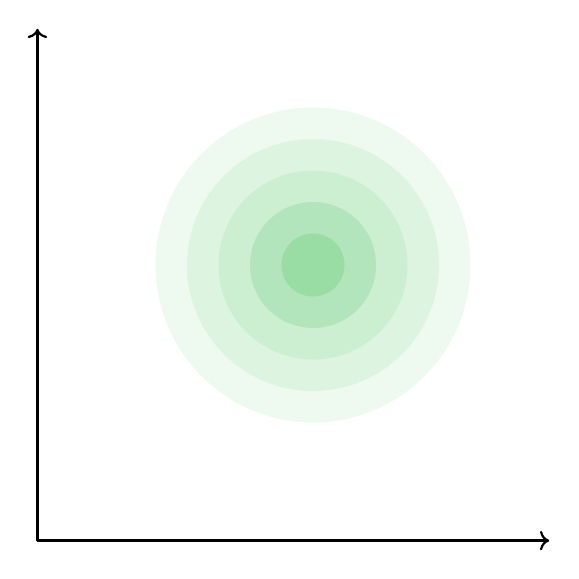
\begin{tikzpicture}
            \draw[thick,->] (-3.5, -3.5) -- (-3.5, 3);
            \draw[thick,->] (-3.5, -3.5) -- (3, -3.5);
            \foreach \x/\alpha in {2/10, 1.6/20, 1.2/30, 0.8/45, 0.4/60}
                \fill[viridisgreen!\alpha] (0, 0) circle (\x);
            %\node[draw, fill=viridisgreen!10] (kde-outer) at (0, 0) {} circle (2) {};
        \end{tikzpicture}
    };
    
    \node[dot, fill=darkgreen!80,
    above right = 0.25cm and 0.3cm of kde,
    label=above:{$h_{\psib}(\x)$}
    ] (s-star) at (kde) {};
    \node[dot, 
    fill=errorcolor!80, 
    below left = -1.5cm and -1.4cm of kde,
    label=below:{$h_{\psib}(\observed{\x})$}
    ] (s-obs) {};
    
    \node[network-box, right = of kde] (inference-network) {$\huge{f_{\phib}}$\\Inference\\Network};
    

    \matrix[right = of inference-network, row sep = 0.2cm] {
    \node[posterior-box, fill=viridisgreen!20]  (correct-posterior) {Correct\\Posterior}; \\ 
    \node[posterior-box, fill=errorcolor!20] (incorrect-posterior) {Incorrect\\Posterior}; \\
    };

    %\node[posterior-box, above right = of inference-network, fill=darkgreen!20] (correct-posterior) {Correct Posterior};
    %\node[posterior-box, below = of correct-posterior, fill=errorcolor!20] (incorrect-posterior) {Incorrect Posterior};
    
    \draw [dashed, thick] (typical-generative-set) -- (x-obs) node [sloped,midway](M){};;
    
    \node[below left = of M] (simulation-gap) {Misspecification};
    \draw [arrow] (simulation-gap)  -- (M);
    
    \node[below left=-2.6cm and -2.6cm of kde] (kde-outer) {};
    \draw [dashed, thick] (s-obs) -- (kde-outer) node [sloped,midway](M2){};;
    
    \node[below right = 2cm and 0.3cm of M2] (simulation-gap-detected) {Misspecification detected};
    \draw [arrow] (simulation-gap-detected)  -- (M2);
    
    
    \draw [arrow, dashed] (x-star) -- (summary-network);
    \draw [arrow, dashed, color=errorcolor] (x-obs) -- (summary-network);
    
    \draw [arrow, dashed] (summary-network) -- (s-star);
    \draw [arrow, color=errorcolor, dashed] (summary-network) -- (s-obs);
    
    %\node[below right = of s-obs] (simulation-gap-detected) {Simulation gap detected};
    %\draw [arrow] (simulation-gap-detected) -- (s-obs);
    
    \draw [arrow, dashed] (s-star) -- (inference-network);
    \draw [arrow, dashed, color=errorcolor] (s-obs) -- (inference-network);
    
    \draw [arrow, dashed] (inference-network) -- (correct-posterior.west);
    \draw [arrow, color=errorcolor, dashed] (inference-network) -- (incorrect-posterior.west);
\end{tikzpicture}

